	
	%Chapter I
	\chapter{Varieries (대수다양체)}
	
	이 장에서 우리의 목표는 가능한 한 최소한의 도구로 대수기하학의 도입을 제시하는 것이다.
	우리는 고정된 대수적으로 닫힌 체 $k$ 상에서 작업할 것이다.
	우리는 주요 연구 대상인 아핀 또는 사영공간에서의 대수다양체를 정의할 것이다.
	우리는 차원, 정칙 함수, 유리함수, 비특이 대수다양체, 사영 대수다양체의 차수와 같은 매우 중요한 개념들을 도입할 것이다.
	또한 우리는 가장 중요한 여러 구체적인 예시를 각 절의 끝에 있는 연습문제의 형태로 제시할 것이다.
	예시들은 책에 언급된 것 이상의 여러 흥미롭고 중요한 현상들을 보여줄 수 있도록 선택되었다.
	이러한 예시들을 주의깊게 탐구하는 사람은 대수기하학의 기본 개념을 잘 이해하게 될뿐만 아니라
	현대 대수기하학의 보다 추상적인 발전을 이해할 수 있는 배경 및 자신의 직관을 확인할 수 있는 자료도 갖게 될 것이다.
	이 책의 남은 부분에서 우리는 지속적으로 이 예제들을 참조할 것이다.
	이 장의 마지막 절은 이 책에 대한 일종의 두 번째 소개입니다.
	여기에는 대수 기하학의 발전에 많은 동기를 부여한 "분류 문제"에 대한 논의가 포함되어 있다.
	이는 또한 대수기하학의 기초를 발전시켜야 하는 일반성의 정도에 대한 논의를 포함하며, 이는 스킴 이론에 대한 동기를 제공한다.
	
	
	%Section I.1
	\section{Affine Varieties (아핀 대수다양체)}
	
	$k$가 대수적으로 닫힌 체라 하자. $k$ 상에서의 \tb{아핀 $n$-공간(affine $n$-space)}을
	$k$의 원소들의 모든 순서 $n$쌍들의 집합으로 정의하며 $\mb A_k^n$ 또는 간단히 $\An$으로 표기한다.
	원소 $P\in\An$은 \tb{점(point)}이라 불릴 것이며 만약 $P=(a_1,\ldots,a_n),a_i\in k$이면
	$a_i$는 $P$의 \tb{좌표(coordinate)}라 불릴 것이다.
	
	$A=k[x_1,\ldots,x_n]$이 $k$ 상에서의 $n$변수 다항식환이라 하자.
	우리는 $f\in A$와 $P\in\An$에 대하여 $f(P)=f(a_1,\ldots,a_n)$이라 정의하는 것으로
	$A$의 원소들을 아핀 $n$-공간에서 $k$로의 함수들로 표현할 것이다.	
	그러므로 만약 $f\in A$가 다항식이면 우리는 $f$의 \tb{영점(zero)}들의 집합 $Z(f)=\sx{P\in\An}{f(P)=0}$을 언급할 수 있다.
	더 일반적으로 만약 $T$가 $A$의 임의의 부분집합이면 $T$의 \tb{영점집합(zero set)}을 $T$의 원소들의 공통 영점들의 집합으로 정의한다.
	%
	$$Z(T)=\sx{P\in\An}{\forall f\in T\;f(P)=0}$$
	%
	명백히 만약 $\mf a$가 $T$에 의해 생성된 $A$의 아이디얼이면 $Z(T)=Z(\mf a)$이다.
	이에 더해 $A$가 Noether 환이므로 임의의 아이디얼 $\mf a$는 유한한 생성집합 $f_1,\ldots,f_r$을 가진다.
	그러므로 $Z(T)$는 다항식들의 유한집합 $f_1,\ldots,f_r$의 공통 영점들에 의해 표현될 수 있다.
	
	
	%Definition
	\begin{definition}
	%
		\tn{$\An$의 부분집합 $Y$가 \tb{대수적 집합(algebraic set)}이라는 것의 정의는
		$Y=Z(T)$를 만족시키는 부분집합 $T\bseq A$가 존재하는 것이다.}
	%
	\end{definition}
	
	
	%Proposition 1.1
	\begin{proposition}
	%
		\tn{\\두 대수적 집합의 합집합은 대수적 집합이다. 대수적 집합들의 임의의 족의 교집합은 대수적 집합이다.
		공집합과 전체 공간은 대수적 집합이다.\\\\
	%
		\pf 만약 $Y_1=Z(T_1)$이며 $Y_2=Z(T_2)$이면 $T_1T_2$가 $T_1$의 원소와 $T_2$의 원소의 임의의 곱들의 집합을 나타낸다면
		$Y_1\cup Y_2=Z(T_1T_2)$이다.
		사실 만약 $P\in Y_1\cup Y_2$이면 $P\in Y_1$ 또는 $P\in Y_2$이므로 $P$는 $T_1T_2$에 속한 모든 다항식의 영점이다.
		역으로 만약 $P\in Z(T_1T_2)$이며 $P\notin Y_1$이면 $f\in T_1$이 존재하여 $f(P)\ne 0$을 만족시킨다.
		이제 임의의 $g\in T_2$에 대하여 $(fg)(P)=0$임은 $g(P)=0$을 함의하며 따라서 $P\in Y_2$이다.\\
		만약 $Y_\al=Z(T_\al)$가 대수적 집합들의 임의의 족이면 $\bigcap Y_\al=Z(\bigcup T_\al)$이며
		따라서 $\bigcap Y_\al$도 대수적 집합이다.
		마지막으로 공집합 $\es=Z(1)$이며 전체 공간 $\An=Z(0)$이다.}
	%
	\end{proposition}
	
	
	%Definition
	\begin{definition}
	%
		\tn{$\An$ 상에서의 \tb{Zariski 위상(Zariski topology)}을 대수적 집합의 여집합들을 열린집합으로 취하여 정의한다.
		위 명제에 의해 두 열린집합의 교집합과 임의의 열린집합족의 합집합이 열린집합이므로 이것은 위상이다.
		이에 더해 공집합과 전체집합은 열린집합이다.}
	%
	\end{definition}
	
	
	%Example 1.1.1
	\begin{example}
	%
		\tn{\\아핀 직선 $\mb A^1$ 상에서의 Zariski 위상을 고려하자.
		$A=k[x]$에서의 모든 아이디얼은 주 아이디얼이고 따라서 모든 대수적 집합은 하나의 다항식의 영점집합이다.
		$k$가 대수적으로 닫혀 있으므로 모든 0이 아닌 다항식 $f(x)$는 $c,a_1,\ldots,a_n\in k$에 대하여
		$f(x)=c(x-a_1)\cdots(x-a_n)$으로 표현될 수 있다. 그 경우 $Z(f)=\{a_1,\ldots,a_n\}$이다.
		그러므로 $\mb A^1$에서의 대수적 집합들은 단지 유한집합(공집합을 포함)들과 ($f=0$에 대응하는) 전체 공간뿐이다.
		따라서 열린집합들은 공집합과 유한 부분집합의 여집합들이다. 특히 이 위상이 Hausdorff가 아님을 기억해 두라.}
	%
	\end{example}
	
	
	%Definition
	\begin{definition}
	%
		\tn{위상공간 $X$의 공집합이 아닌 부분집합 $Y$가 \tb{기약(irreducible)}이라는 것의 정의는
		$Y$에서 닫혀 있는 두 진부분집합의 합집합 $Y=Y_1\cup Y_2$로 표현 불가능한 것이다. 공집합은 기약이라 간주된다.}
	%
	\end{definition}
	
	
	%Example 1.1.2
	\begin{example}
	%
		\tn{\\$\mb A^1$의 닫힌 진부분집합은 유한집합뿐이지만 $\mb A^1$은 무한집합이므로
		($k$가 대수적으로 닫혀 있는 체이므로 무한체이다) $\mb A^1$은 기약이다.}
	%
	\end{example}
	
	
	%Example 1.1.3
	\begin{example}
	%
		\tn{\\기약 공간의 임의의 공집합이 아닌 열린 부분집합은 기약이며 조밀하다.}
	%
	\end{example}
	
	
	%Example 1.1.4
	\begin{example}
	%
		\tn{\\만약 $Y$가 $X$의 기약 부분집합이면 그 $X$에서의 폐포 $\bar Y$도 기약이다.}
	%
	\end{example}
	
	
	%Definition
	\begin{definition}
	%
		\tn{\tb{아핀 대수다양체(affine algebraic variety)}(또는 간단히 \tb{affine variety})는
		(유도된 위상을 가지는) $\An$의 기약 닫힌 부분집합이다.
		아핀 대수다양체의 열린 부분집합은 \tb{준아핀 대수다양체(quasi-affine variety)}이다.}
	%
	\end{definition}
	
	이러한 아핀 및 준아핀 대수다양체가 우리의 첫 번째 탐구 대상이다.
	그러나 더 나아가기 전에, 심지어 어떠한 흥미로운 예를 제시하기 전에
	우리는 $\An$의 부분집합과 $A$의 아이디얼 간의 관계를 더 깊이 탐구할 필요가 있다.
	그러므로 임의의 부분집합 $Y\bseq\An$에 대하여 $Y$의 $A$에서의 \tb{아이디얼(ideal)}을 다음과 같이 정의한다.
	%
	$$I(Y)=\sx{f\in A}{\forall P\in Y\;f(P)=0}$$
	%
	이제 우리는 $A$의 부분집합을 대수적 집합으로 대응시키는 함수 $Z$와
	$\An$의 부분집합들을 아이디얼로 대응시키는 함수 $I$를 가지고 있다. 이들의 성질들은 다음 명제에 요약되어 있다.
	
	
	%Proposition 1.2
	\begin{proposition}
	%
		\tn{\begin{enumerate}[label=(\alph*)]
		\item 만약 $T_1\bseq T_2$가 $A$의 부분집합이면 $Z(T_1)\pseq Z(T_2)$이다.
		\item 만약 $Y_1\bseq Y_2$가 $\An$의 부분집합이면 $I(Y_1)\pseq I(Y_2)$이다.
		\item $\An$의 임의의 두 부분집합 $Y_1,Y_2$에 대하여 $I(Y_1\cup Y_2)=I(Y_1)\cap I(Y_2)$가 성립한다.
		\item 임의의 아이디얼 $\mf a\bseq A$에 대하여 $I(Z(\mf a))=\sqrt{\mf a}$ ($\mf a$의 근기)이다.
		\item 임의의 부분집합 $Y\bseq\An$에 대하여 $Z(I(Y))=\bar Y$ ($Y$의 폐포)이다.
		\end{enumerate}}
	%
		\tn{\\\pf (a), (b), (c)는 자명하다. $\mf a$의 근기가 다음과 같이 정의되므로
		(d)는 아래에 기술된 Hilbert 영점 정리의 직접적인 결과이다.}
	%
		$$\sqrt{\mf a}=\sx{f\in A}{\exists r>0\;f^r\in\mf a}$$
	%
		\tn{(e)를 증명하기 위해 $Y\bseq Z(I(Y))$이며 이것이 닫힌집합임을 기억해 두라. 따라서 $\bar Y\bseq Z(I(Y))$이다.
		반면에 $W$가 $Y$를 포함하는 임의의 닫힌집합이라 하자. 그 경우 어떠한 아이디얼 $\mf a$에 대하여 $W=Z(\mf a)$이다.
		그러므로 $Z(\mf a)\pseq Y$이고 (b)에 의해 $I(Z(\mf a))\bseq I(Y)$이다.
		그러나 명백히 $\mf a\bseq I(Z(\mf a))$이므로 (a)에 의해 $W=Z(\mf a)\pseq Z(I(Y))$이다. 그러므로 $Z(I(Y))=\bar Y$이다.}
	%
	\end{proposition}
	
	
	%Theorem 1.3A
	\begin{theorema}[Hilbert's Nullstellensatz (Hilbert 영점 정리)]
	%
		\tn{\\$k$가 대수적으로 닫힌 체이고 $\mf a$가 $A=k[x_1,\ldots,x_n]$에서의 아이디얼이며
		$f\in A$가 $Z(\mf a)$의 모든 점에서 소멸하는 다항식이라 하자. 그 경우 어떠한 정수 $r>0$에 대하여 $f^r\in\mf a$이다.\\\\
	%
		\pf Lang [2, p. 256] 또는 Atiyah-Macdoanld [1, p. 85] 또는 Zariski-Samuel [1. vol. 2, p. 164]}
	%
	\end{theorema}
	
	
	%Corollary 1.4
	\begin{corollary}
	%
		\tn{\\$\An$에서의 대수적 집합들과 $A$에서의 \tb{근기 아이디얼(radical ideal)}(i.e. 자신의 근기와 일치하는 아이디얼)들 간에
		$Y\mt I(Y)$와 $\mf a\mt Z(\mf a)$로 주어진 포함 관계를 역전시키는 일대일 대응이 존재한다.
		이에 더해 대수적 집합이 기약일 필요충분조건은 그 아이디얼이 소 아이디얼인 것이다.\\\\
	%
		\pf 마지막 부분만이 새로운 정보이다. 만약 $Y$가 기약이면 $I(Y)$가 소 아이디얼임을 보이자.
		만약 $fg\in I(Y)$이면 $Y\bseq Z(fg)=Z(f)\cup Z(g)$이다.
		그러므로 $Y=(Y\cap Z(f))\cup(Y\cap Z(g))$이며 두 부분집합은 $Y$의 닫힌 부분집합이다.
		$Y$가 기약이므로 $Y=Y\cap Z(f)$(이 경우 $Y\bs Z(f)$) 또는 $Y=Y\cap Z(g)$(이 경우 $Y\bs Z(g)$)이다.
		따라서 $f\in I(Y)$ 또는 $g\in I(Y)$이다.\\
		역으로 $\mf p$가 소 아이디얼이라 하고 $Z(\mf p)=Y_1\cup Y_2$라 하자.
		그 경우 $\mf p=I(Y_1)\cap I(Y_2)$이며 따라서 $\mf p=I(Y_1)$ 또는 $\mf p=I(Y_2)$이다.
		그러므로 $Z(\mf p)=Y_1$ 또는 $Y_2$이며 따라서 이는 기약이다.}
	%
	\end{corollary}
	
	
	%Example 1.4.1
	\begin{example}
	%
		\tn{\\$\An$은 $A$에서의 소 아이디얼인 0 아이디얼에 대응하므로 기약이다.}
	%
	\end{example}
	
	
	%Example 1.4.2
	\begin{example}
	%
		\tn{\\$f$가 $A=k[x,y]$에서의 기약다항식이라 하자.
		그 경우 $A$가 유일 인수분해 정역이므로 $f$는 $A$에서의 소 아이디얼을 생성하며 따라서 영점집합 $Y=Z(f)$는 기약이다.
		우리는 이를 방정식 $f(x,y)=0$에 의해 정의된 \tb{아핀 곡선(affine curve)}이라 부른다.
		만약 $f$가 $d$차이면 $Y$가 \tb{$d$차(degree $d$)} 곡선이라 한다.}
	%
	\end{example}
	
	
	%Example 1.4.3
	\begin{example}
	%
		\tn{\\더 일반적으로 만약 $f$가 $A=k[x_1,\ldots,x_n]$에서의 기약다항식이면 아핀 대수다양체 $Y=Z(f)$를 얻는다.
		이는 $n=3$의 경우 \tb{곡면(surface)}, $n>3$일 경우 \tb{초곡면(hypersurface)}이라 불린다.}
	%
	\end{example}
	
	
	%Example 1.4.4
	\begin{example}
	%
		\tn{\\$A=k[x_1,\ldots,x_n]$의 극대 아이디얼 $\mf m$은 $\An$의 극소 기약 닫힌 부분집합에 대응한다.
		이는 점 $P=(a_1,\ldots,a_n)$이어야 한다. 이것은 $A$의 모든 극대 아이디얼이
		어떠한 $a_1,\ldots,a_n\in k$에 대하여 $\mf m=(x_1-a_1,\ldots,x_n-a_n)$ 형태여야 함을 보여준다.}
	%
	\end{example}
	
	
	%Example 1.4.5
	\begin{example}
	%
		\tn{\\만약 $k$가 대수적으로 닫혀 있지 않다면 이러한 결과는 성립하지 않는다.
		예를 들어 $k=\R$일 경우 $\mb A_\R^2$에서의 곡선 $x^2+y^2+1=0$은 점을 갖지 않는다.
		따라서 (1.2d)는 거짓이다. (Ex. 1.12)를 참조하라.}
	%
	\end{example}
	
	
	%Definition
	\begin{definition}
	%
		\tn{만약 $Y\bseq\An$이 아핀 대수적 집합이면 $Y$의 \tb{아핀 좌표환(affine coordinate ring)} $A(Y)$를 $A/I(Y)$로 정의한다.}
	%
	\end{definition}
	
	
	%Remark 1.4.6
	\begin{remark}
	%
		\tn{\\만약 $Y$가 아핀 대수다양체이면 $A(Y)$는 정역이다. 이에 더해 $A(Y)$는 유한생성 $k$-대수이다.
		역으로 정역인 임의의 유한생성 $k$-대수 $B$는 어떠한 아핀 대수다양체의 아핀 좌표환이다:
		$B$를 다항식환 $A=k[x_1,\ldots,x_n]$의 아이디얼 $\mf a$에 의한 몫환으로 표현하고 $Y=Z(\mf a)$라 하라.}
	%
	\end{remark}
	
	
	다음으로 우리는 대수다양체의 위상을 탐구할 것이다.
	이를 위해 우리는 모든 대수다양체를 포함하는 위상공간들의 중요한 부류를 도입할 것이다.
	
	
	%Definition
	\begin{definition}
	%
		\tn{\\위상공간 $X$가 \tb{Noether(Noetherian)}라는 것의 정의는 닫힌집합들에 대한
		\tb{하강 연쇄 조건(descending chain condition)}을 만족시키는 것이다:
		임의의 닫힌집합열 $Y_1\pseq Y_2\pseq\cdots$에 대하여 정수 $r$이 존재하여 $Y_r=Y_{r+1}=\cdots$를 만족시킨다.}
	%
	\end{definition}
	
	
	%Example 1.4.7
	\begin{example}
	%
		\tn{\\$\An$은 Noether 위상공간이다: 만약 $Y_1\pseq Y_2\pseq\cdots$가 닫힌집합들의 하강 연쇄이면
		$I(Y_1)\bseq I(Y_2)\bseq\cdots$는 $A=k[x_1,\ldots,x_n]$의 아이디얼들의 상승 연쇄이다.
		$A$가 Noether 환이므로 이러한 아이디얼들의 연쇄는 궁극적으로 상승을 멈출 것이다.
		그러나 각각의 $i$에 대하여 $Y_i=Z(I(Y_i))$이므로 연쇄 $Y_i$도 궁극적으로 하강을 멈출 것이다.}
	%
	\end{example}
	
	
	%Proposition 1.5
	\begin{proposition}
	%
		\tn{\\Noether 위상 공간 $X$에서 공집합이 아닌 모든 닫힌 부분집합 $Y$는 기약 닫힌 부분집합 $Y_i$들의 유한 합집합
		$Y=Y_1\cup\cdots\cup Y_r$로 표현 가능하다.
		만약 $i\ne j$이면 $Y_i\not\pseq Y_j$임을 요구한다면 $Y_i$들은 유일하게 결정된다.
		이들은 $Y$의 \tb{기약 성분(irreducible component)}들이라 불린다.\\\\
	%
		\pf 먼저 우리는 이러한 $Y$의 표현이 존재함을 보일 것이다.
		$\mf S$가 $X$의 공집합이 아닌 닫힌 부분집합 중 기약 닫힌 부분집합들의 유한 합집합으로 표현 불가능한 것들의 집합이라 하자.
		만약 $\mf S$가 공집합이 아니면 $X$가 Noether이므로 이는 극소원 $Y$를 포함해야 한다.
		$\mf S$의 구축에 의해 $Y$는 기약이 아니다. 그러므로 $Y$의 닫힌 진부분집합 $Y',Y''$에 대하여 $Y=Y'\cup Y''$으로 표현 가능하다.
		$Y$의 극소성에 의해 $Y'$과 $Y''$은 기약 닫힌 부분집합들의 유한 합집합으로 표현 가능하며 따라서 $Y$도 그러하므로 모순이다.
		그러므로 모든 닫힌집합 $Y$는 기약 부분집합들의 합집합 $Y=Y_1\cup\cdots\cup Y_r$로 표현 가능하다 결론지을 수 있다.
		필요하다면 일부를 제거하는 것으로 우리는 $i\ne j$이면 $Y_i\not\pseq Y_j$라 가정할 수 있다.\\
		이제 $Y=Y_1'\cup\cdots\cup Y_s'$이 이러한 다른 표현이라 하자.
		그 경우 $Y_1'\bseq Y=Y_1\cup\cdots\cup Y_r$이므로 $Y_1'=\bigcup(Y_1'\cap Y_i)$이다.
		그러나 $Y_1'$은 기약이므로 어떠한 $i$에 대하여 $Y_1'\bseq Y_i$이다. 예를 들어 $i=1$이라 하자.
		마찬가지로 어떠한 $j$에 대하여 $Y_1\bseq Y_j'$이다.
		그 경우 $Y_1'\bseq Y_j'$이며 따라서 $j=1$이다. 그러므로 $Y_1=Y_1'$이 성립한다.
		이제 $Z=\overline{(Y-Y_1)}$이라 하자. 그 경우 $Z=Y_2\cup\cdots\cup Y_t$이며 $Z=Y_2'\cup\cdots\cup Y_s'$이다.
		$r$에 대한 귀납법을 진행하면 $Y_i$의 유일성을 얻는다.}
	%
	\end{proposition}
	
	
	%Corollary 1.6
	\begin{corollary}
	%
		\tn{\\$\An$에서의 모든 대수적 집합은 서로를 포함하지 않는 대수다양체들의 합집합으로 유일하게 표현 가능하다.}
	%
	\end{corollary}
	
	
	%Definition
	\begin{definition}
	%
		\tn{\\만약 $X$가 위상공간이면 $X$의 \tb{차원(dimension)}을 ($\dim X$로 표기하며) $X$의 서로 다른 기약 닫힌 부분집합들의 연쇄
		$Z_0\bs Z_1\bs\cdots\bs Z_n$이 존재하도록 하는 모든 정수 $n$의 상한으로 정의한다.
		아핀 또는 준아핀 대수다양체의 \tb{차원(dimension)}을 그 위상공간으로서의 차원으로 정의한다.}
	%
	\end{definition}
	
	
	%Example 1.6.1
	\begin{example}
	%
		\tn{\\$\mb A^1$의 차원은 1이다: $\mb A^1$의 기약 닫힌 부분집합들은 점들과 전체 공간뿐이다.}
	%
	\end{example}
	
	
	%Definition
	\begin{definition}
	%
		\tn{환 $A$에서 소 아이디얼 $\mf p$의 \tb{높이(height)}는 서로 다른 소 아이디얼들의 연쇄
		$\mf p_0\bs\mf p_1\bs\cdots\bs\mf p_n=\mf p$가 존재하도록 하는 모든 정수 $n$의 상한이다.
		$A$의 \tb{차원(dimension)}(또는 \tb{Krull 차원(Krull dimension)})을 모든 소 아이디얼의 높이들의 상한으로 정의한다.}
	%
	\end{definition}
	
	
	%Proposition 1.7
	\begin{proposition}
	\tn{\\만약 $Y$가 아핀 대수적 집합이면 $Y$의 차원은 그 아핀 좌표환 $A(Y)$의 차원과 같다.\\\\
	%
	\pf 만약 $Y$가 $\An$에서의 아핀 대수적 집합이면 $Y$의 기약 닫힌 부분집합들은
	$I(Y)$를 포함하는 $A=k[x_1,\ldots,x_n]$의 소 아이디얼에 대응된다. 이는 다시 $A(Y)$의 소 아이디얼에 대응된다.
	따라서 $\dim Y$는 $A(Y)$에 속한 소 아이디얼들의 연쇄의 최장 길이이며 이는 $A(Y)$의 차원이다.}
	\end{proposition}
	
	이 명제는 Noether 환에 대한 차원론의 결과를 대수기하학에 적용할 수 있도록 해 준다.
	
	
	%Theorem 1.8A
	\begin{theorema}
	%
		\tn{\\$k$가 체이며 $B$가 정역인 유한생성 $k$-대수라 하자. 그 경우 다음이 성립한다:\\[-2mm]
	%
		\begin{enumerate}[label=(\alph*)]
		\item $B$의 차원은 $B$의 $k$ 상에서의 분수체 $K(B)$의 초월 차수와 동일하다.
		\item $B$에서의 임의의 소 아이디얼 $\mf p$에 대하여 다음이 성립한다.
		\end{enumerate}}
	%
		$$\mrm{height}\;\mf p+\dim B/\mf p=\dim B$$
	%
		\tn{\pf Matsumura [2, Ch. 5, \S 14] 또는 $k$가 대수적으로 닫혀 있는 경우 Atiyah-Macdonald [1, Ch 11]}
	%
	\end{theorema}
	
	
	%Proposition 1.9
	\begin{proposition}
	%
		\tn{\\$\An$의 차원은 $n$이다.\\\\
	%
		\pf (1.7)에 의해 이는 다항식환 $k[x_1,\ldots,x_n]$의 차원이 $n$임과 동치이다.
		이는 위 정리의 (a)에서 따라온다.}
	%
	\end{proposition}
	
	
	%Proposition 1.10
	\begin{proposition}
	%
		\tn{\\만약 $Y$가 준아핀 대수다양체이면 $\dim Y=\dim\bar Y$이다.\\\\
	%
		\pf 만약 $Z_0\bs Z_1\bs\cdots\bs Z_n$이 $Y$의 서로 다른 기약 닫힌 부분집합들의 열이면
		$\bar Z_0\bs\bar Z_1\bs\cdots\bs\bar Z_n$은 $\bar Y$의 서로 다른 기약 닫힌 부분집합들의 열이다. (1.1.4)
		따라서 $\dim Y\le\dim\bar Y$이다.
		특히 $\dim Y$가 유한하므로 우리는 $n=\dim Y$인 극대 연쇄 $Z_0\bs\cdots\bs Z_n$을 선택할 수 있다.
		이 경우 $Z_0$는 점 $P$여야 하며 연쇄 $P=\bar Z_0\bs\cdots\bs\bar Z_n$도 극대가 될 것이다. (1.1.3)
		이제 $P$는 $\bar Y$의 아핀 좌표환 $A(\bar Y)$의 극대 아이디얼 $\mf m$에 대응한다.
		$\bar Z_i$는 $\mf m$에 포함된 소 아이디얼에 대응하며 따라서 $\mrm{height}\;\mf m=n$이다.
		반면에 $P$가 아핀 공간의 점이므로 $A(\bar Y)/\mf m\cong k$이다. (1.4.4)
		따라서 (1.8Ab)에 의해 $n=\dim A(\bar Y)=\dim\bar Y$이다. 그러므로 $\dim Y=\dim\bar Y$이다.}
	%
	\end{proposition}
	
	
	%Theorem 1.11A
	\begin{theorema}[Krull's Hauptidealsatz (Krull 주 아이디얼 정리)]
	%
		\tn{\\$A$가 Noether 환이며 $f\in A$가 영인자도 가역원도 아닌 원소라 하자.
		그 경우 $f$를 포함하는 모든 극소 소 아이디얼 $\mf p$는 높이 1이다.\\\\
	%
		\pf Atiyah-Macdonald [1, p. 122]}
	%
	\end{theorema}
	
	
	%Proposition 1.12A
	\begin{propositiona}
	%
		\tn{\\Noether 정역 $A$가 유일 인수분해 정역일 필요충분조건은 높이 1인 모든 소 아이디얼이 주 아이디얼인 것이다.\\\\
	%
		\pf Matsumura [2, p. 141] 또는 Bourbaki [1, Ch. 7, \S 3]}
	%
	\end{propositiona}
	
	
	%Proposition 1.13
	\begin{proposition}
	%
		\tn{\\$\An$에서의 대수다양체 $Y$가 차원 $n-1$을 가질 필요충분조건은
		$A=k[x_1,\ldots,x_n]$에 속한 상수다항식이 아닌 하나의 기약다항식의 영점집합 $Z(f)$인 것이다.\\\\
	%
		\pf 만약 $f$가 기약다항식이면 $Z(f)$가 대수다양체임을 보였다. 그 아이디얼은 소 아이디얼 $\mf p=(f)$이다,
		(1.11A)에 의해 $\mf p$는 높이 1이며 따라서 (1.8A)에 의해 $Z(f)$는 $n-1$차원이다.
		역으로 $n-1$차원 다양체는 높이 1의 소 아이디얼에 대응된다.
		이제 다항식환 $A$가 유일 인수분해 정역이므로 (1.12A)에 의해
		$\mf p$는 주 아이디얼이며 하나의 기약다항식 $f$에 의해 생성되어야 한다. 따라서 $Y=Z(f)$이다.}
	%
	\end{proposition}
	
	
	%Remark 1.13.1
	\begin{remark}
	%
		\tn{\\다항식환에서의 높이 2인 소 아이디얼은 두 개의 원소에 의해 생성되지 못할 수도 있다. (Ex. 1.11)}
	%
	\end{remark}
	
	
	\subsection*{Exercises (연습문제)}
	
	
	\begin{enumerate}[label=\tb{1.\arabic*.},itemindent=0mm,itemsep=2mm]
	\item \begin{enumerate}[label=(\alph*)]
	\item $Y$가 평면 곡선 $y=x^2$라 하자. (i.e. $Y$는 다항식 $f=y-x^2$의 영점집합이다.)
	$A(Y)$가 $k$ 상에서의 1변수 다항식환과 동형임을 보여라.
	\item $Z$가 평면 곡선 $xy=1$이라 하자. $A(Z)$가 $k$ 상에서의 1변수 다항식환과 동형이 아님을 보여라.
	\end{enumerate}
	\begin{enumerate}[label=*(\alph*)]
	\setcounter{enumii}{2}
	\item $f$가 $k[x,y]$에 속한 임의의 기약 2차 다항식이며 $W$가 $f$에 의해 정의된 원뿔곡선이라 하자.
	$A(W)$가 $A(Y)$ 또는 $A(Z)$와 동형임을 보여라. 각각 어떠한 경우인가?
	\end{enumerate}
	\item \tb{비틀린 3차곡선(twisted cubic curve)}. $Y\bseq\mb A^3$이 집합 $\sx{(t,t^2,t^3)}{t\in k}$라 하자.
	$Y$가 1차원 아핀 대수다양체임을 보여라. 아이디얼 $I(Y)$의 생성자들을 찾아라.
	$A(Y)$가 $k$ 상에서의 1변수 다항식환과 동형임을 보여라.
	(이 경우 $Y$가 \tb{매개변수 표현(parametric representation)} $x=t,y=t^2,z=t^3$에 의해 주어졌다고 한다.)
	\item $Y$가 두 다항식 $x^2-yz$와 $xz-x$에 의해 주어진 $\mb A^3$에서의 대수적 집합이라 하자.
	$Y$가 세 기약 성분의 합집합임을 보여라. 이들을 기술하고 이들의 소 아이디얼들을 찾아라.
	\item $\mb A^2$를 $\mb A^1\times\mb A^1$과 자연스러운 방법으로 동일시한다면
	$\mb A^2$ 상에서의 Zariski 위상이 $\mb A^1$의 두 사본 상에서의 Zariski 위상들의 곱위상이 아님을 보여라.
	\item $k$-대수 $B$가 어떤 $n$에 대하여 $\An$에서의 어떠한 대수적 집합의 아핀 좌표환과 동형일 필요충분조건은
	$B$가 멱영원을 갖지 않는 유한생성 $k$-대수인 것임을 보여라.
	\item 기약 위상공간의 임의의 공집합이 아닌 열린 부분집합은 조밀하며 기약이다.
	만약 $Y$가 위상공간 $X$의 부분집합이며 그 유도 위상 하에서 기약이면 폐포 $\bar Y$도 기약이다.
	\item \begin{enumerate}[label=(\alph*)]
	\item 위상공간 $X$에 대한 다음의 조건들이 동치임을 보여라:
	\begin{enumerate}[label=(\roman*)]
	\item $X$는 Noether이다.
	\item 닫힌 부분집합들의 모든 공집합이 아닌 족은 극소원을 가진다.
	\item $X$는 열린 부분집합들에 대한 상승 연쇄 조건을 만족시킨다.
	\item 열린 부분집합들의 모든 공집합이 아닌 족은 극대원을 가진다.
	\end{enumerate}
	\item Noether 위상 공간은 \tb{준컴팩트(quasi-compact)}이다. 즉 모든 열린 덮개가 유한 부분덮개를 가진다.
	\item Noether 위상 공간의 임의의 부분집합은 유도 위상 하에서 Noether이다.
	\item Hausdorff 공간인 Noether 공간은 이산위상을 가진 유한집합이어야 한다.
	\end{enumerate}
	\item $Y$가 $\An$에서의 $r$차원 아핀 대수다양체라 하자. $H$가 $\An$에서의 초곡면이며 $Y\not\bseq H$라 하자.
	그 경우 $Y\cap H$의 모든 기약 성분은 $r-1$차원이다. (일반화는 (7.1)을 참조하라.)
	\item $\mf a\bseq A=k[x_1,\ldots,x_n]$이 $r$개 원소에 의해 생성될 수 있는 아이디얼이라 하자.
	그 경우 $Z(\mf a)$의 모든 기약 성분은 $n-r$차원 이상이다.
	\item \begin{enumerate}[label=(\alph*)]
	\item 만약 $Y$가 위상공간 $X$의 임의의 부분집합이면 $\dim Y\le\dim X$이다.
	\item 만약 $X$가 열린 부분집합들의 족 $\{U_i\}$에 의해 덮이는 위상공간이라면 $\dim X=\sup\dim U_i$이다.
	\item $\dim U<\dim X$인 위상공간 $X$와 조밀 열린 부분집합 $U$의 예를 제시하라.
	\item 만약 $Y$가 기약 유한 차원 위상공간 $X$의 닫힌 부분집합이며 $\dim Y=\dim X$이면 $Y=X$이다.
	\item 무한 차원 Noether 위상 공간의 예를 제시하라.
	\end{enumerate}
	\end{enumerate}
	\begin{enumerate}[label=\tb{*1.\arabic*.},itemindent=0mm,topsep=2mm]
	\setcounter{enumi}{10}
	\item $Y\bseq\mb A^3$이 매개변수방정식 $x=t^3,y=t^4,z=t^5$에 의해 주어진 곡선이라 하자.
	$I(Y)$가 $k[x,y,z]$에서의 높이 2인 아이디얼이며 2개 원소에 의해 생성될 수 없음을 보여라.
	우리는 $Y$가 \tb{국소 완비 교집합(local complete intersection)}이 아니라고 한다 - cf. (Ex. 2.17)
	\end{enumerate}
	\begin{enumerate}[label=\tb{1.\arabic*.},itemindent=0mm,itemsep=2mm,topsep=2mm]
	\setcounter{enumi}{11}
	\item 영점집합 $Z(f)$가 $\mb A_\R^2$에서 기약이 아닌 기약다항식 $f\in\R[x,y]$의 예를 제시하라. (cf. 1.4.2)
	\end{enumerate}
	
	
	
	%Section I.2
	\section{Projective Varieties (사영 대수다양체)}
	
	사영 대수다양체를 정의하기 위해 우리는 (사영공간에서 작업한다는 점을 제외하면) 아핀 대수다양체와 유사한 과정을 진행할 것이다.
	
	$k$가 고정된 대수적으로 닫힌 체라 하자. $k$ 상에서의 \tb{사영 $n$-공간(projective $n$-space)}을
	$\mb P_k^n$ 또는 간단히 $\Pn$으로 표기하며 전부 0이지는 않은 $k$의 원소들의 순서 $n+1$조 $(a_0,\ldots,a_n)$의
	$(a_0,\ldots,a_n)\sim(\lm a_0,\ldots,\lm a_n)\;(\forall\lm\in k,\lm\ne 0)$에 의해 주어진
	동치 관계 하에서의 동치류들의 집합으로 정의한다.
	이를 표현하는 다른 방법은 $\Pn$이 집합으로서 집합 $\mb A^{n+1}-\{(0,\ldots,0)\}$의
	원점을 지나는 동일한 직선 상에 놓이는 점들을 동일화하는 동치 관계 하에서의 몫이라는 것이다.
	
	$\Pn$의 원소는 점이라 불린다. 만약 $P$가 점이면 동치류 $P$에 속한 임의의 순서 $n+1$조 $(a_0,\cdots,a_n)$은
	\tb{$P$에 대한 동차 좌표들의 집합(set of homogeneous coordinates for $P$)}라 한다.
	
	$S$가 다항식환 $k[x_0,\cdots,x_n]$이라 하자. 우리는 $S$를 등급환으로 취급하고자 한다.
	따라서 우리는 등급환의 개념을 간단히 상기하겠다.
	
	\tb{등급환(graded ring)}은 임의의 $d,e\ge 0$에 대하여 $S_d\cdot S_e\bseq S_{d+e}$를 만족시키는
	가환군 $S_d$들의 직접합으로의 분해 $S=\bigoplus_{d\ge 0}S_d$를 가지는 환 $S$이다.
	$S_d$의 원소는 \tb{$d$차 동급 원소(homogeneous element of degree $d$)}(다항식환의 경우 \tb{동차 원소})라 불린다.
	그러므로 $S$의 임의의 원소는 동급 원소들의 유한합으로 유일하게 표현될 수 있다.
	아이디얼 $\mf a\bseq S$가 \tb{동급 아이디얼(homogeneous ideal)}(다항식환의 경우 \tb{동차 아이디얼})이라는 것의 정의는
	$\mf a=\bigoplus_{d\ge 0}(\mf a\cap S_d)$인 것이다.
	우리는 동급 아이디얼에 대한 몇 가지 기본적인 사실들을 필요로 할 것이다.
	(예를 들어 Matsumura [2, \S 10] 또는 Zariski-Samuel [1, vol. 2, Ch. VII, \S 2]를 참조하라.)
	아이디얼이 동급일 필요충분조건은 동급 원소들에 의해 생성될 수 있는 것이다.
	동급 아이디얼의 합, 곱, 교집합, 근기는 동급이다. 동급 아이디얼이 소 아이디얼인지 결정하기 위해서는
	임의의 두 \ti{동급} 원소 $f,g$에 대하여 $fg\in\mf a$가 $f\in\mf a$ 또는 $g\in\mf a$를 함의하는지를 보이면 충분하다.
	
	우리는 $S_d$를 $x_0,\ldots,x_n$에 대한 총 차수 $d$인 단항식들의 모든 선형결합들의 집합으로 취하는 것으로
	다항식환 $S=k[x_0,\ldots,x_n]$을 등급환으로 만들 것이다.
	만약 $f\in S$가 다항식이면 동차 좌표들이 불균일하므로 $\Pn$ 상에서의 함수를 정의하기 위해 사용할 수 없다.
	그러나 만약 $f$가 $d$차 동차다항식이면 $f(\lm a_0,\ldots,\lm a_n)=\lm^df(a_0,\ldots,a_n)$이므로
	$f$가 0이 되는지 그렇지 않은지에 관한 성질은 $(a_0,\ldots,a_n)$의 동치류에만 의존한다.
	그러므로 $f$는 $f(a_0,\ldots,a_n)=0$이면 $f(P)=0$이고
	$f(a_0,\ldots,a_n)\ne 0$이면 $f(P)=1$인 $\Pn$에서 $\{0,1\}$로의 함수를 제공한다.
	
	그러므로 우리는 동차다항식의 \tb{영점(zero)}들, 즉 $Z(f)=\sx{P\in\Pn}{f(P)=0}$에 대해 논할 수 있다.
	만약 $T$가 $S$의 동차 원소들의 임의의 집합이면 $T$의 \tb{영점집합(zero set)}은 다음과 같다.
	%
	$$Z(T)=\sx{P\in\Pn}{\forall f\in T\;f(P)=0}$$
	%
	만약 $\mf a$가 $S$의 동차 아이디얼이면 $T$가 $\mf a$에 속한 모든 동차 원소들의 집합이라 할 때 $Z(\mf a)=Z(T)$로 정의한다.
	$S$가 Noether 환이므로 동차 원소들의 집합 $T$의 유한 부분집합 $f_1,\ldots,f_r$이 존재하여 $Z(T)=Z(f_1,\ldots,f_r)$을 만족시킨다.
	
	
	%Definition
	\begin{definition}
	%
		\tn{$\Pn$의 부분집합 $Y$가 \tb{대수적 집합(algebraic set)}이라는 것의 정의는
		$S$의 동급 원소들의 집합 $T$가 존재하여 $Y=Z(T)$를 만족시키는 것이다.}
	%
	\end{definition}
	
	
	%Proposition 2.1
	\begin{proposition}
	%
		\tn{\\두 대수적 집합의 합집합은 대수적 집합이다. 대수적 집합들의 임의의 족의 교집합은 대수적 집합이다.
		공집합과 전체 공간은 대수적 집합이다.\\\\
	%
		\pf 독자에게 남긴다. (위의 (1.1)의 증명과 유사하다.)}
	%
	\end{proposition}
	
	
	%Definition
	\begin{definition}
	%
		\tn{$\Pn$ 상에서의 \tb{Zariski 위상(Zariski topology)}을 대수적 집합의 여집합들을 열린집합으로 취하는 것으로 정의한다.}
	%
	\end{definition}
	
	위상공간을 가진다면 \S 1에서 정의된 기약 부분집합과 부분집합의 차원의 개념이 적용된다.
	
	
	%Definition
	\begin{definition}
	%
		\tn{\tb{사영 대수다양체(projective algebraic variety)}(또는 간단히 \tb{projective variety})는
		유도된 위상을 가지는 $\Pn$에서의 기약 대수적 집합이다.
		사영 대수다양체의 열린 부분집합은 \tb{준사영 대수다양체(quasi-projective variety)}이다.
		사영 또는 준사영 대수다양체의 \tb{차원(dimension)}은 그 위상공간으로서의 차원이다.\\
		만약 $Y$가 $\Pn$의 부분집합이면 $Y$의 $S$에서의 \tb{동차 아이디얼(homogeneous ideal)}을 $I(Y)$로 표기하며
		$\sx{f\in S}{f\text{가 동차이며 }\forall P\in Y\;f(P)=0}$에 의해 생성되는 아이디얼로 정의한다.
		만약 $Y$가 대수적 집합이면 $Y$의 \tb{동차 좌표환(homogeneous coordinate ring)}을 $S(Y)=S/I(Y)$로 정의한다.
		사영공간에서의 대수적 집합과 그 동차 아이디얼들의 여러 성질에 대해서는 아래의 (Ex. 2.1 - 2.7)로 남기겠다.}
	%
	\end{definition}
	
	우리의 다음 목표는 사영 $n$-공간이 아핀 $n$-공간들에 의한 열린 덮개를 가짐을 보이며
	따라서 모든 사영(resp. 준사영) 대수다양체가 아핀(resp. 준아핀) 대수다양체들에 의한 열린 덮개를 가짐을 보이는 것이다.
	먼저 우리는 몇 가지 표기법을 도입하겠다.
	
	만약 $f\in S$가 1차 동차다항식이면 $f$의 영점집합은 \tb{초평면(hyperplane)}이라 불린다.
	특히 우리는 $i=0,\ldots,n$에 대하여 $x_i$의 영점집합을 $H_i$로 표기할 것이다.
	$U_i$가 열린집합 $\Pn-H_i$라 하자. 그 경우 $\Pn$은 열린집합 $U_i$들에 의해 덮인다:
	만약 $P=(a_0,\ldots,a_n)$이 점이면 적어도 하나의 $a_i\ne 0$이며 따라서 $P\in U_i$이다.
	함수 $\ph_i:U_i\ra\An$을 다음과 같이 정의한다:
	만약 $P=(a_0,\ldots,a_n)\in U_i$이면 $\ph_i(P)=Q$는 다음과 같은 좌표를 가지는 점이다.
	%
	$$\left(\frac{a_0}{a_i},\ldots,\frac{a_n}{a_i}\right)$$
	%
	($a_i/a_i$ 제외) 비 $a_j/a_i$들이 동차 좌표의 선택에 독립적이므로 $\ph_i$가 잘 정의됨을 기억해 두라.
	
	
	%Proposition 2.2
	\begin{proposition}
	%
		\tn{\\함수 $\ph_i$는 유도 위상이 부여된 $U_i$에서 Zariski 위상이 부여된 $\An$으로의 위상동형사상이다.\\\\
	%
		\pf 명백히 $\ph_i$는 전단사이므로 $U_i$의 닫힌집합들이 $\ph_i$에 의해 $\An$의 닫힌집합들과 동일화됨을 보이면 충분하다.
		$i=0$이라 가정하고 $U_0$을 $U$로, $\ph_0$를 $\ph:U\ra\An$으로 표기하겠다.\\
		$A=k[x_1,\ldots,x_n]$이라 하자.
		우리는 $S$의 동차 원소들의 집합 $S^h$에서 $A$로의 함수 $\al$와 $A$에서 $S^h$로의 함수 $\be$를 정의할 것이다.
		주어진 $f\in S^h$에 대하여 $\al(f)=f(1,y_1,\ldots,y_n)$으로 설정한다.
		반면에 주어진 $e$차 다항식 $g\in A$에 대하여 $x_0^eg(x_1/x_0,\ldots,x_n/x_0)$는
		$x_i$에 대한 $e$차 동차다항식이며 우리는 이를 $\be(g)$라 부를 것이다.\\
		이제 $Y\bseq U$가 닫힌 부분집합이라 하자. $\bar Y$가 그 $\Pn$에서의 폐포라 하자.
		이는 대수적 집합이므로 어떠한 부분집합 $T\bseq S^h$에 대하여 $\bar Y=Z(T)$이다.
		$T'=\al(T)$라 하자. 그 경우 직접 확인하면 $\ph(Y)=Z(T')$임을 알 수 있다.
		역으로 $W$가 $\An$의 닫힌 부분집합이라 하자. 그 경우 $A$의 어떠한 부분집합 $T'$에 대하여 $W=Z(T')$이며
		$\ph^{-1}(W)=Z(\be(T'))\cap U$임을 간단히 확인할 수 있다.
		그러므로 $\ph$와 $\ph^{-1}$은 모두 닫힌 함수이며 따라서 $\ph$는 위상동형사상이다.}
	%
	\end{proposition}
	
	
	%Corollary 2.3
	\begin{corollary}
	%
		\tn{\\만약 $Y$가 사영(resp. 준사영) 대수다양체이면 $Y$는 열린집합 $Y\cap U_i,i=0,\ldots,n$에 의해 덮인다.
		이들은 위에서 정의된 함수 $\ph_i$에 의해 아핀(resp. 준아핀) 대수다양체와 동형이다.}
	%
	\end{corollary}
	
	
	
	\subsection*{Exercises (연습문제)}
	
	
	\begin{enumerate}[label=\tb{2.\arabic*.},itemindent=0mm,itemsep=2mm]
	\item $\mf a\bseq S$가 동차 아이디얼이며 $f\in S$가 $\deg f>0$이며
	모든 $P\in Z(\mf a)\bseq\Pn$에 대하여 $f(P)=0$을 만족시키는 동차다항식이면
	어떠한 $q>0$에 대하여 $f^q\in\mf a$라 기술하는 '동차 영점 정리'를 증명하라.
	[Hint: 문제를 아핀 좌표환이 $S$인 아핀 $(n+1)$-공간에 대하여 표현하고 통상적인 영점 정리 (1.3A)를 적용하라.]
	\item 동차 아이디얼 $\mf a\bseq S$에 대하여 다음 조건들이 동치임을 보여라:
	\begin{enumerate}[label=(\roman*)]
		\item $Z(\mf a)=\es$ (공집합)
		\item $\sqrt{\mf a}=S$ 또는 아이디얼 $S_+=\bigoplus_{d>0}S_d$
		\item 어떠한 $d>0$에 대하여 $\mf a\pseq S_d$
	\end{enumerate}
	\item \begin{enumerate}[label=(\alph*)]
	\item 만약 $T_1\bseq T_2$가 $S^h$의 부분집합이면 $Z(T_1)\pseq Z(T_2)$이다.
	\item 만약 $Y_1\bseq Y_2$가 $\P^n$의 부분집합이면 $I(Y_1)\pseq I(Y_2)$이다.
	\item $\Pn$의 임의의 두 부분집합 $Y_1,Y_2$에 대하여 $I(Y_1\cup Y_2)=I(Y_1)\cap I(Y_2)$이다.
	\item 만약 $\mf a\bseq S$가 $Z(\mf a)\ne\es$인 동차 아이디얼이면 $I(Z(\mf a))=\sqrt{\mf a}$이다.
	\item 임의의 부분집합 $Y\bseq\Pn$에 대하여 $Z(I(Y))=\bar Y$이다.
	\end{enumerate}
	\item \begin{enumerate}[label=(\alph*)]
	\item $\Pn$에서의 대수적 집합들과 $S_+$를 제외한 $S$의 동차 근기 아이디얼들 간에는
	$Y\mt I(Y)$와 $\mf a\mt Z(\mf a)$로 주어진 포함 관계를 반전하는 일대일대응이 존재한다.
	Note: $S_+$가 이 대응에서 나타나지 않으므로 이는 때로는 $S$의 \tb{무관(irrelevant)} 극대 아이디얼이라 불린다.
	\item 대수적 집합 $Y\bseq\Pn$이 기약일 필요충분조건은 $I(Y)$가 소 아이디얼인 것이다.
	\item $\Pn$ 자신이 기약임을 보여라.
	\end{enumerate}
	\item \begin{enumerate}[label=(\alph*)]
	\item $\Pn$은 Noether 위상 공간이다.
	\item $\Pn$에서의 모든 대수적 집합은 서로를 포함하지 않는 기약 대수적 집합들의
	유한 합집합으로 유일하게 표현될 수 있다. 이들은 \tb{기약 인자(irreducible component)}라 불린다.
	\end{enumerate}
	\item 만약 $Y$가 동차 좌표환 $S(Y)$를 가지는 사영 대수다양체이면 $\dim S(Y)=\dim Y+1$임을 보여라.
	[Hint: $\ph_i:U_i\ra\An$이 (2.2)의 위상동형사상이며
	$Y_i$가 아핀 대수다양체 $\ph_i(Y\cap U_i)$이고 $A(Y)$가 그 아핀 좌표환이라 하라.
	$A(Y_i)$가 국소화 환 $S(Y)_{x_i}$의 차수 0인 원소들의 부분환과 동일시될 수 있음을 보여라.
	그 후 $S(Y)_{x_i}\cong A(Y_i)[x_i,x_i^{-1}]$임을 보여라.
	이제 (1.7), (1.8A), (Ex. 1.10)을 사용하고 초월 차수를 관찰하라.
	또한 $Y_i$가 공집합이 아닐 경우 $\dim Y=\dim Y_i$라고 결론지어라.]
	\item \begin{enumerate}[label=(\alph*)]
	\item $\dim\Pn=n$
	\item 만약 $Y\bseq\Pn$이 준사영 대수다양체이면 $\dim Y=\dim\bar Y$이다.
	\end{enumerate}
	$[$Hint: 문제를 (1.10)으로 줄이기 위해 (Ex 2.6)을 사용하라.$]$
	\item 사영 대수다양체 $Y\bseq\Pn$이 $n-1$차원일 필요충분조건은 하나의 양의 차수의 기약 동차다항식 $f$의 영점집합인 것이다.
	$Y$는 $\Pn$에서의 \tb{초곡면(hypersurface)}이라 불린다.
	\item \tb{아핀 대수다양체의 사영 폐포}. 만약 $Y\bseq\An$이 아핀 다양체이면
	위상동형사상 $\ph_0$에 의해 $\An$을 열린집합 $U_0\bseq\Pn$과 동일시한다.
	그 경우 우리는 $Y$의 \tb{사영 폐포(projective closure)}라 불리는 $\Pn$에서의 폐포 $\bar Y$를 논할 수 있다.
	\begin{enumerate}[label=(\alph*)]
	\item (2.2)의 증명에서의 표기법을 사용하여 $I(\bar Y)$가 $\be(I(Y))$에 의해 생성된 아이디얼임을 보여라.
	\item $Y\bseq\mb A^3$이 (Ex. 1.2)의 비틀린 3차곡선이라 하자.
	그 사영 폐포 $\bar Y\bseq\mb P^3$은 $\mb P^3$에서의 \tb{비틀린 3차곡선(twisted cubic curve)}이라 불린다.
	$I(Y)$와 $I(\bar Y)$의 생성자들을 찾고 이 예를 이용해 만약 $f_1,\ldots,f_r$이 $I(Y)$를 생성하더라도
	$\be(f_1),\ldots,\be(f_r)$이 $I(\bar Y)$를 생성할 필요는 \ti{없음을} 보여라.
	\end{enumerate}
	\item \tb{사영 대수다양체 상에서의 뿔} (Fig. 1).
	$Y\bseq\Pn$이 공집합이 아닌 대수적 집합이며 $\ta:\mb A^{n+1}-\{(0,\ldots,0)\}\ra\Pn$이
	아핀 좌표 $(a_0,\ldots,a_n)$인 점을 동차 좌표 $(a_0,\ldots,a_n)$인 점으로 대응시키는 함수라 하자.
	$Y$ 상에서의 \tb{아핀 뿔(affine cone)}을 다음과 같이 정의한다.
	%
	$$C(Y)=\ta^{-1}(Y)\cup\{(0,\ldots,0)\}$$
	%
	\begin{enumerate}[label=(\alph*)]
	\item $C(Y)$가 $\mb A^{n+1}$에서의 대수적 집합이며 그 아이디얼이
	($k[x_0,\ldots,x_n]$에서의 통상적인 아이디얼로 간주될 경우) $I(Y)$와 같음을 보여라.
	\item $C(Y)$가 기약일 필요충분조건은 $Y$가 기약인 것이다.
	\item $\dim C(Y)=\dim Y+1$
	\end{enumerate}
	때로는 $C(Y)$의 $\mb P^{n+1}$에서의 사영 폐포 $\overline{C(Y)}$를 고려한다.
	이는 $Y$ 상에서의 \tb{사영 뿔(projective cone)}이라 불린다.
	\end{enumerate}
	%
	\newpage
	%Figure 1
	\begin{center}
		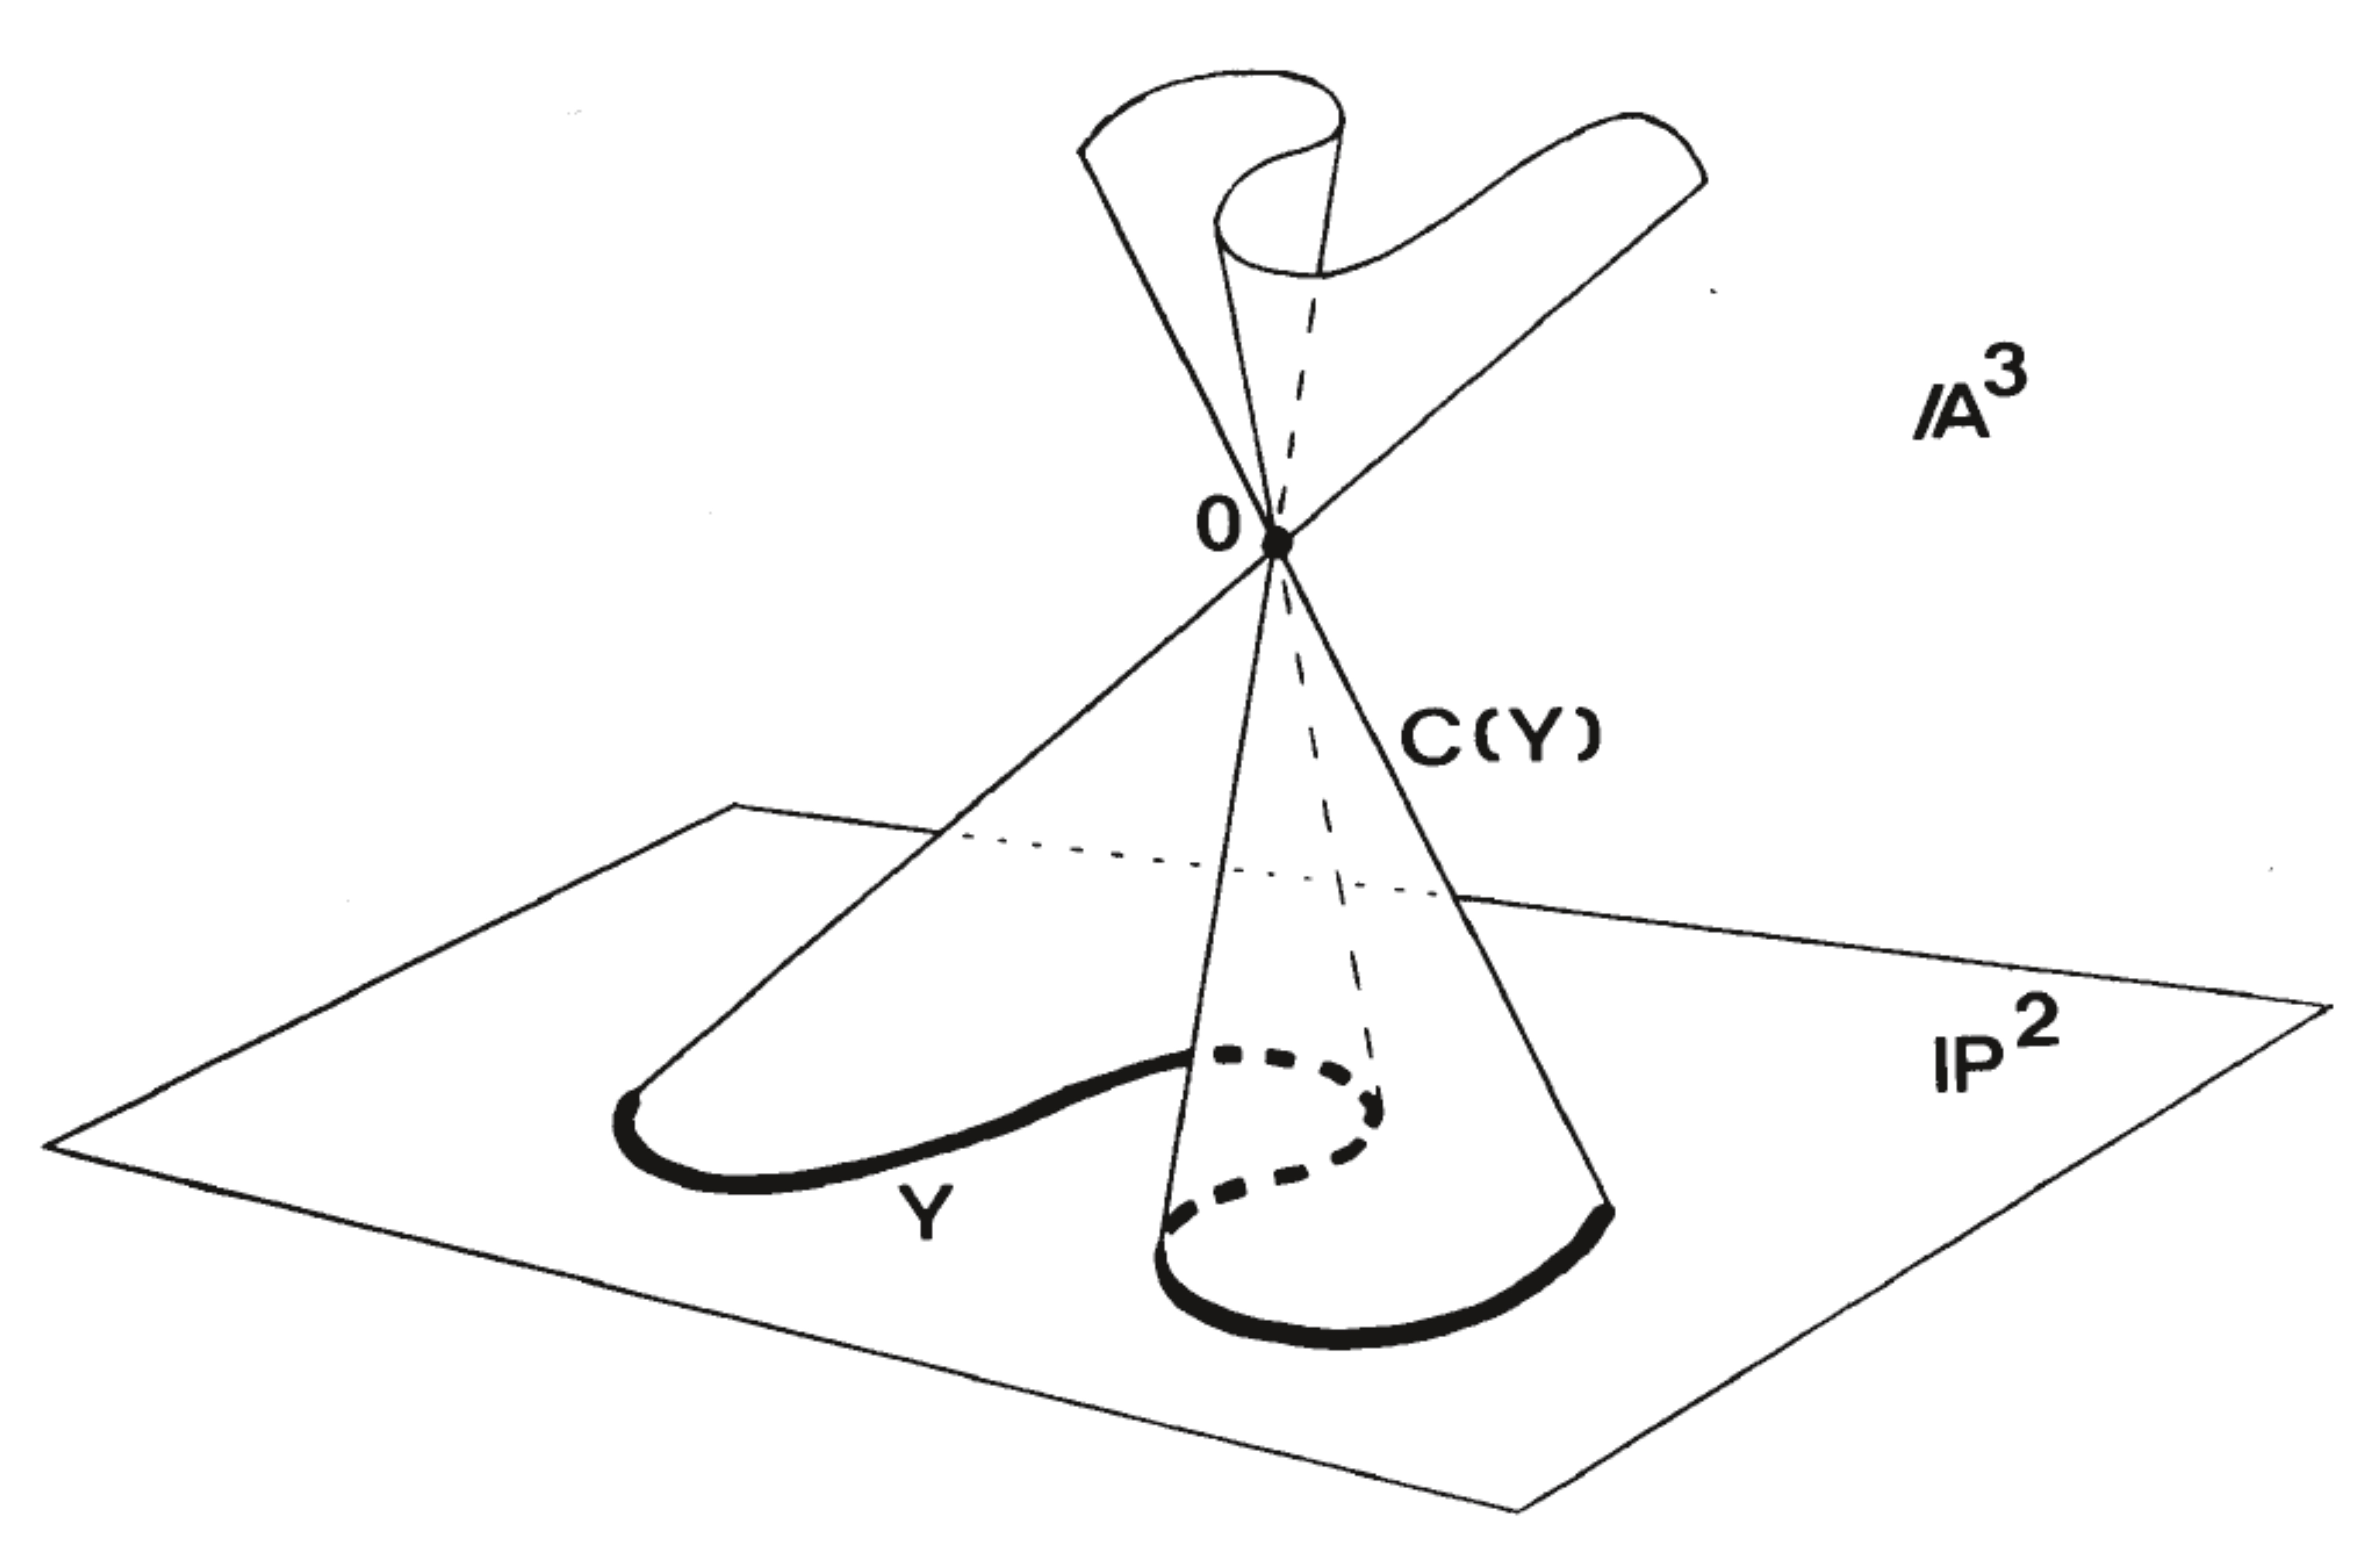
\includegraphics[width=0.5\columnwidth]{Figure1}\\
		Figure 1. $\mb P^2$에서의 곡선 상에서의 뿔
	\end{center}
	%
	\begin{enumerate}[label=\tb{2.\arabic*.},itemindent=0mm,itemsep=2mm]
	\setcounter{enumi}{10}
	\item \tb{$\Pn$에서의 선형 대수다양체}. 1차다항식에 의해 정의된 초곡면은 \tb{초평면(hyperplane)}이라 불린다.
	\begin{enumerate}[label=(\alph*)]
	\item $\Pn$에서의 대수다양체 $Y$에 대한 다음 두 조건이 동치임을 보여라:
	\begin{enumerate}[label=(\roman*)]
	\item $I(Y)$는 1차다항식들에 의해 생성될 수 있다.
	\item $Y$는 초평면들의 교집합으로 표현될 수 있다.
	\end{enumerate}
	이 경우 우리는 $Y$가 $\Pn$에서의 \tb{선형 대수다양체(linear variety)}라 한다.
	\item 만약 $Y$가 $\Pn$에서의 $r$차원 선형 대수다양체이면
	$I(Y)$가 최소 $n-r$개의 1차다항식에 의해 생성됨을 보여라.
	\item $Y,Z$가 $\Pn$에서의 선형 대수다양체이며 $\dim Y=r,\dim Z=s$라 하자.
	만약 $r+s-n\ge 0$이면 $Y\cap Z\ne\es$이다.
	이에 더해 만약 $Y\cap Z\ne\es$이면 $Y\cap Z$는 차원 $r+s-n$ 이상의 선형 대수다양체이다.
	($\mb A^{n+1}$을 $k$ 상에서의 벡터 공간으로 간주하고 그 부분공간에서 작업하라.)
	\end{enumerate}
	\item \tb{$d$차 매장}. 주어진 $n,d>0$에 대하여 $M_0,M_1,\ldots,M_N$이
	$n+1$개 변수 $x_0,\ldots,x_n$에 대한 모든 $d$차 단항식들이라 하자. 여기에서 $N=\binom{n+d}{n}-1$이다.
	함수 $\rho_d:\Pn\ra\mb P^N$을 점 $P=(a_0,\ldots,a_n)$을 단항식 $M_j$들에 $a_i$들을 대입하여 얻어진
	점 $\rho_d(P)=(M_0(a),\ldots,M_N(a))$로 대응시키는 함수로 정의하자.
	이는 $\Pn$에서 $\mb P^N$으로의 \tb{$d$차 매장($d$-uple embedding)}이라 불린다.
	예를 들어 만약 $n=1,d=2$이면 $N=2$이고 $\mb P^1$의 $\mb P^2$로의 $2$차 매장의 상 $Y$는 원뿔곡선이다.
	\begin{enumerate}[label=(\alph*)]
	\item $\ta:k[y_0,\ldots,y_N]\ra k[x_0,\ldots,x_n]$이
	$y_i$를 $M_i$로 대응시키는 것으로 정의된 준동형사상이며 $\mf a$가 $\ta$의 핵이라 하자.
	그 경우 $\mf a$는 동차 소 아이디얼이며 따라서 $Z(\mf a)$는 $\mb P^N$에서의 사영 대수다양체이다.
	\item $\rho_d$의 상이 정확히 $Z(\mf a)$임을 보여라. (한쪽 포함 관계는 간단하다. 반대쪽은 계산이 필요하다.)
	\item 이제 $\rho_d$가 $\Pn$에서 사영 대수다양체 $Z(\mf a)$로의 위상동형사상임을 보여라.
	\item $\mb P^3$에서의 비틀린 3차곡선(Ex. 2.9)이 적절한 좌표 선택 하에서
	$\mb P^1$의 $\mb P^3$으로의 3차 매장과 동일함을 보여라.
	\end{enumerate}
	\item $Y$가 $\mb P^2$의 $\mb P^5$로의 2차 매장의 상이라 하자. 이는 \tb{Veronese 곡면(Veronese surface)}이다.
	만약 $Z\bseq Y$가 폐곡선이면(\tb{곡선(curve)}은 1차원 대수다양체이다)
	$V\cap Y=Z$를 만족시키는 초곡면 $V\bseq\mb P^5$가 존재함을 보여라.
	\item \tb{Segre 매장}. $\psi:\mb P^r\times\mb P^s\ra\mb P^N$이 순서 쌍 $(a_0,\ldots,a_r)\times(b_0,\ldots,b_s)$를
	사전 순서인 $(\ldots,a_ib_j,\ldots)$로 대응시키는 것으로 정의된 함수라 하자. 여기에서 $N=rs+r+s$이다.
	$\psi$가 잘 정의되었으며 단사임을 기억해 두라. 이는 \tb{Segre 매장(Segre embedding)}이라 불린다.
	$\psi$의 상이 $\mb P^N$의 \tb{부분대수다양체(subvariety)}임을 보여라.
	[Hint: $\mb P^N$의 동차 좌표가 $\sx{z_{ij}}{i=0,\ldots,r,j=0,\ldots,s}$라 하고
	$\mf a$가 $z_{ij}$를 $x_iy_j$로 대응시키는 준동형사상 $k[\{z_{ij}\}]\ra k[x_0,\ldots,x_r,y_0,\ldots,y_s]$의 핵이라 하자.
	그 후 $\Im\psi=Z(\mf a)$임을 보여라]
	\item \tb{$\mb P^3$에서의 2차곡면} (Fig. 2). 방정식 $xy-zw=0$에 의해 정의된 $\mb P^3$에서의 곡면 $Q$를 고려하자.
	(\tb{곡면(surface)}은 2차원 대수다양체이다.)
	\begin{enumerate}[label=(\alph*)]
	\item $Q$가 적절한 좌표 선택 하에서 $\mb P^1\times\mb P^1$의 $\mb P^3$으로의 Segre 매장과 동일함을 보여라.
	\item $Q$가 $t\in\mb P^1$에 의해 매개화된 다음을 만족시키는 직선들의 두 개의 족 $\{L_t\},\{M_t\}$를 포함함을 보여라:
	(\tb{직선(line)}은 1차원 선형 대수다양체이다.)
	만약 $L_t\ne L_u$이면 $L_t\cap L_u=\es$, 만약 $M_t\ne M_u$이면 $M_t\cap M_u=\es$,
	모든 $t,u$에 대하여 $L_t\cap M_u=$ 한 점.
	\item $Q$가 이러한 직선들 이외에도 다른 곡선들을 포함함을 보이고 $Q$ 상에서의 Zariski 위상이
	$\mb P^1\times\mb P^1$ 상에서의 곱위상(여기에서 각각의 $\mb P^1$은 Zariski 위상을 가진다.)과
	$\psi$를 통해 위상동형이 아님을 보여라.
	\end{enumerate}
	\end{enumerate}
	%
	%Figure 2
	\begin{center}
	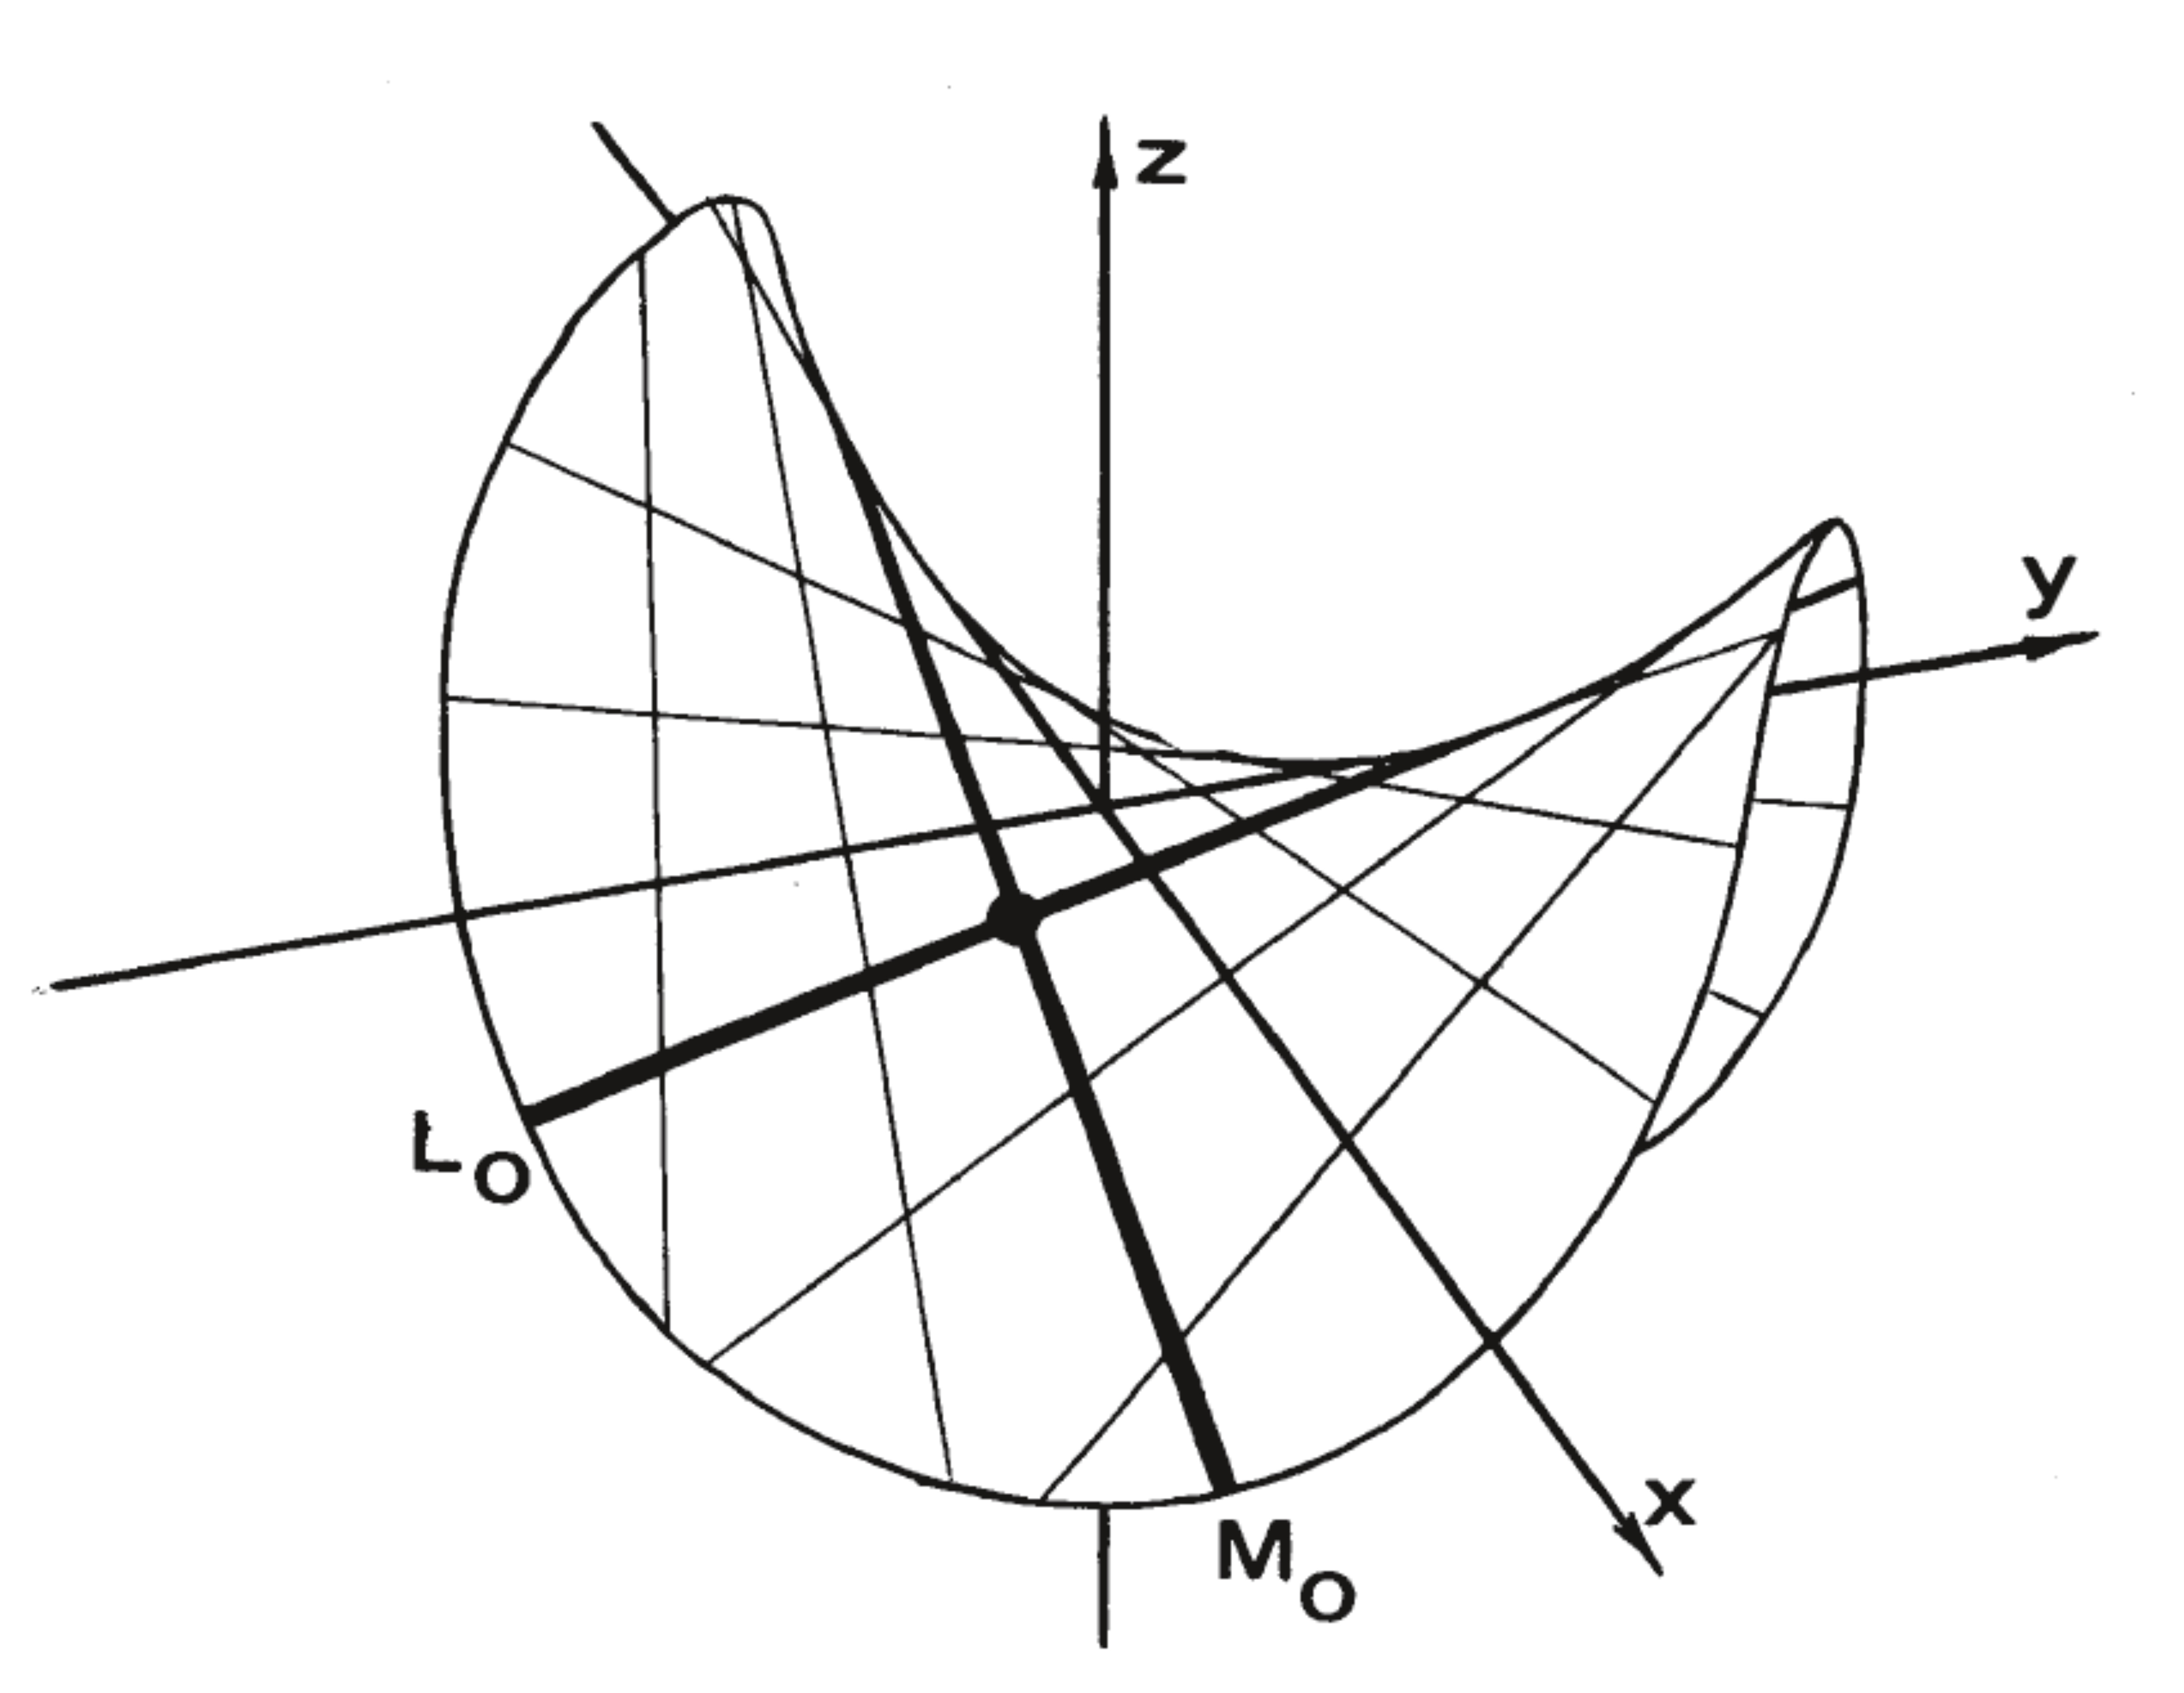
\includegraphics[width=0.5\columnwidth]{Figure2}\\
	Figure 2. $\mb P^3$에서의 2차곡면
	\end{center}
	%
	\begin{enumerate}[label=\tb{2.\arabic*.},itemindent=0mm,itemsep=2mm]
	\setcounter{enumi}{15}
	\item \begin{enumerate}[label=(\alph*)]
	\item 두 대수다양체의 교집합이 대수다양체여야 할 필요는 없다.
	예를 들어 $Q_1$과 $Q_2$가 각각 방정식 $x^2-yw=0$과 $xy-zw=0$에 의해 주어진 $\mb P^3$에서의 2차곡면이라 하자.
	$Q_1\cap Q_2$가 비틀린 3차곡선과 직선의 합집합임을 보여라.
	\item 두 대수다양체의 교집합이 대수다양체이더라도 교집합의 아이디얼은 아이디얼들의 합이 아닐 수 있다.
	예를 들어 $C$가 방정식 $x^2-yz=0$에 의해 주어진 $\mb P^2$에서의 2차곡선이라 하자.
	$L$이 $y=0$에 의해 주어진 직선이라 하자. $C\cap L$이 한 점 $P$로 구성되어 있지만 $I(C)+I(L)\ne I(P)$임을 보여라.
	\end{enumerate}
	\item \tb{완비 교집합}. $\Pn$에서의 $r$차원 대수다양체 $Y$가 \tb{(강)완비 교집합((strict) complete intersection)}이라는
	것의 정의는 $I(Y)$가 $n-r$개 원소에 의해 생성될 수 있는 것이다.
	$Y$가 \tb{집합론적 완비 교집합(set-theoretic complete intersection)}이라는 것의 정의는
	$Y$가 $n-r$개 초곡면의 교집합으로 표현 가능한 것이다.
	\begin{enumerate}[label=(\alph*)]
	\item $Y$가 $\Pn$에서의 대수다양체이며 $Y=Z(\mf a)$라 하자. 또한 $\mf a$가 $q$개 원소에 의해 생성될 수 있다 하자.
	그 경우 $\dim Y\ge n-q$임을 보여라.
	\item 강완비 교집합이 집합론적 완비 교집합임을 보여라.
	\end{enumerate}
	\begin{enumerate}[label=*(\alph*)]
	\setcounter{enumii}{2}
	\item (b)의 역은 거짓이다. 예를 들어 $Y$가 $\mb P^3$에서의 비틀린 3차곡선이라 하자. (Ex. 2.9)
	$I(Y)$가 두 원소에 의해 생성될 수 없음을 보여라.
	반면에 $Y=H_1\cap H_2$를 만족시키는 각각 2차와 3차인 초곡면 $H_1,H_2$를 찾아라.
	\end{enumerate}
	\begin{enumerate}[label=**(\alph*)]
	\setcounter{enumii}{3}
	\item $\mb P^3$에서의 모든 닫힌 기약 곡선이 두 곡면의 집합론적 교집합인지는 아직 해결되지 않은 문제이다.
	해설에 대해서는 Hartshorne [1]과 Hartshorne [5, III, \S 5]를 참조하라.
	\end{enumerate}
	\end{enumerate}
	
	
	
	%Section I.3
	\section{Morphisms (사상)}
	
	지금까지 우리는 아핀 및 사영 대수다양체를 정의했지만 우리는 이들 간에 어떠한 사상이 허용되었는지는 논의하지 않았다.
	우리는 심지어 어떠한 경우에 두 대수다양체가 동형인지도 언급하지 않았다.
	이 절에서 우리는 대수다양체 상에서의 정칙 함수에 대해 논의하고 대수다양체의 사상을 정의할 것이다.
	그러므로 우리는 작업을 수행할 좋은 범주를 얻게 될 것이다.
	
	$Y$가 $\An$에서의 준아핀 대수다양체라 하자. 우리는 $Y$에서 $k$로의 함수 $f$들을 고려할 것이다.
	
	
	%Definition
	\begin{definition}
	%
		\tn{함수 $f:Y\ra k$가 \tb{점 $P\in Y$에서 정칙(regular at a point $P\in Y$)}이라는 것의 정의는
		$P\in U\bseq Y$를 만족시키는 열린 근방 $U$와 다항식 $g,h\in A=k[x_1,\ldots,x_n]$이 존재하여
		$h$가 $U$ 상에서 영점을 갖지 않으며 $U$ 상에서 $f=g/h$인 것이다.
		(여기에서 물론 우리는 다항식을 $\An$ 상에서의 함수로 해석하며 따라서 이는 $Y$ 상에서의 함수이다.)
		$f$가 \tb{$Y$ 상에서 정칙(regular on $Y$)}이라는 것의 정의는 $Y$의 모든 점에서 정칙인 것이다.}
	%
	\end{definition}
	
	
	%Lemma 3.1
	\begin{lemma}
	%
		\tn{\\$k$가 Zariski 위상을 가지는 $\mb A_k^1$과 동일시될 경우 정칙 함수는 연속이다.\\\\
	%
		\pf 닫힌집합의 $f$에 의한 역상이 닫힌집합임을 보이면 충분하다.
		$\mb A_k^1$의 닫힌집합들은 유한 개 점들이므로
		임의의 $a\in k$에 대하여 $f^{-1}(a)=\sx{P\in Y}{f(P)=a}$가 닫혀 있음을 보이면 충분하다.
		이는 국소적으로 확인될 수 있다: 위상공간 $Y$의 부분집합 $Z$가 닫혀 있을 필요충분조건은
		$Z\cap U$가 $U$에서 닫혀 있도록 하는 열린 부분집합 $U$들에 의해 $Y$가 덮일 수 있는 것이다.
		그러므로 $U$가 $f$가 $g,h\in A$에 대하여 $g/h$로 표현될 수 있으며 $h$가 $U$ 상에서 영점을 갖지 않도록 하는 열린집합이라 하자.
		그 경우 $f^{-1}(a)\cap U=\sx{P\in U}{g(P)/h(P)=a}$이다.
		그러나 $g(P)/h(P)=a$ iff $(g-ah)(P)=0$이다. 그러므로 $f^{-1}(a)\cap U=Z(g-ah)\cap U$이며 이는 닫힌집합이다.
		따라서 $f^{-1}(a)$는 $Y$에서 닫혀 있다.}
	%
	\end{lemma}
	
	이제 준사영 대수다양체 $Y\bseq\Pn$을 고려하자.
	
	
	%Definition
	\begin{definition}
	%
		\tn{함수 $f:Y\ra k$가 \tb{점 $P\in Y$에서 정칙(regular at a point $P\in Y$)}이라는 것의 정의는
		$P\in U\bseq Y$를 만족시키는 열린 근방 $U$와 같은 차수의 동차다항식 $g,h\in A=k[x_0,\ldots,x_n]$이 존재하여
		$h$가 $U$ 상에서 영점을 갖지 않으며 $U$ 상에서 $f=g/h$인 것이다.
		(이 경우 $g$와 $h$가 $\Pn$ 상에서의 함수가 아님에도 불구하고 이들이 같은 차수의 동차다항식이므로
		$h\ne 0$이면 이들의 몫이 잘 정의됨을 기억해 두라.)
		$f$가 \tb{$Y$ 상에서 정칙(regular on $Y$)}이라는 것의 정의는 $Y$의 모든 점에서 정칙인 것이다.}
	%
	\end{definition}
	
	
	%Remark 3.1.1
	\begin{remark}
	%
		\tn{\\준아핀 경우와 마찬가지로 정칙 함수는 반드시 연속해야 한다. (증명은 독자에게 남긴다.)
		이것의 중요한 결과는 만약 $f$와 $g$가 대수다양체 $X$ 상에서의 정칙 함수들이며
		어떠한 공집합이 아닌 열린 부분집합 $U\bseq X$ 상에서 $f=g$이면 모든 곳에서 $f=g$라는 것이다:
		$f-g=0$인 점들의 집합은 닫힌 조밀 집합이므로 $X$와 같다.}
	%
	\end{remark}
	
	이제 우리는 대수다양체의 범주를 정의할 수 있다.
	
	
	%Definition
	\begin{definition}
	%
		\tn{$k$가 고정된 대수적으로 닫힌 체라 하자. \tb{$k$ 상에서의 대수다양체(variety over $k$)}%
		(또는 간단히 \tb{대수다양체(variety)})는 위에서 정의한 임의의 아핀, 준아핀, 사영, 준사영 대수다양체이다.
		만약 $X,Y$가 두 대수다양체이면 \tb{사상(morphism)} $\ph:X\ra Y$는 모든 열린집합 $V\bseq Y$와
		임의의 정칙 함수 $f:V\ra k$에 대하여 함수 $f\circ\ph:\ph^{-1}(V)\ra k$가 정칙이도록 하는 연속 함수이다.}
	%
	\end{definition}
	
	명백히 두 사상의 합성은 사상이며 따라서 우리는 범주를 얻는다. 특히 동형사상의 개념을 얻는다:
	두 대수다양체 간의 \tb{동형사상(isomorphism)} $\ph:X\ra Y$는 $\psi\circ\ph=\id_X$와 $\ph\circ\psi=\id_Y$를 만족시키는
	역사상 $\psi:Y\ra X$를 가지는 사상이다.
	동형사상은 반드시 전단사이며 쌍연속이어야 하지만 전단사 쌍연속 사상이 동형사상이어야 할 필요는 없음을 기억해 두라. (Ex. 3.2)\\
	
	이제 우리는 임의의 대수다양체에 연관된 어떠한 함수들의 환을 도입할 것이다.
	
	
	%Definition
	\begin{definition}
	%
		\tn{$Y$가 대수다양체라 하자. $Y$ 상에서의 모든 정칙 함수들의 환을 $\mc O(Y)$로 표기한다.
		만약 $P$가 $Y$에서의 점이면 \tb{$P$의 $Y$ 상에서의 국소환(local ring of $P$ on $Y$)}
		$\mc O_{P,Y}$(또는 간단히 $\mc O_P$)를 $P$ 근처에서 $Y$ 상에서의 정칙 함수들의 \tb{싹(germ)}들의 환으로 정의한다.
		다른 말로 하면 $\mc O_P$의 원소는 $P$를 포함하는 $Y$의 열린 부분집합 $U$와 $U$ 상에서의 정칙 함수 $f$의 쌍 $\bk{U,f}$이며
		$U\cap V$ 상에서 $f=g$일 경우 두 쌍 $\bk{U,f}$와 $\bk{V,g}$를 동일시한다.
		(이것이 동치 관계임을 검증하기 위해 (3.1.1)을 사용하라.)}
	%
	\end{definition}
	
	$\mc O_P$가 실제로 국소환임을 기억해 두라: 그 극대 아이디얼 $\mf m$은 $P$에서 소멸하는 정칙 함수들의 싹들의 집합이다.
	(만약 $f(P)\ne 0$이면 $1/f$는 $P$의 어떠한 근방에서 정칙이다.)
	잉여류체 $\mc O_P/\mf m$은 $k$와 동형이다.
	
	
	%Definition
	\begin{definition}
	%
		\tn{만약 $Y$가 대수다양체이면 $Y$의 \tb{함수체(function field)} $K(Y)$를 다음과 같이 정의한다:
		$K(Y)$의 원소는 $Y$의 공집합이 아닌 열린 부분집합 $U$와 $U$ 상에서의 정칙 함수 $f$의 쌍 $\bk{U,f}$의 동치류들이다;
		만약 $U\cap V$ 상에서 $f=g$이면 두 쌍 $\bk{U,f}$와 $\bk{V,g}$를 동일시한다.
		$K(Y)$의 원소들은 $Y$ 상에서의 \tb{유리함수(rational function)}들이라 불린다.}
	%
	\end{definition}
	
	$K(Y)$가 실제로 체임을 기억해 두라. $Y$가 기약이므로 임의의 두 공집합이 아닌 열린집합은 공집합이 아닌 교집합을 가진다.
	따라서 우리는 $K(Y)$에서 덧셈과 곱셈을 정의할 수 있으며 $K(Y)$는 환이 된다.
	그 경우 만약 $\bk{U,f}\in K(Y)$이며 $f\ne 0$이면 우리는 $f$를 열린집합 $V=U-U\cap Z(f)$로 제한할 수 있으며
	이곳에서 $f$는 영점을 갖지 않고 따라서 $1/f$는 $V$ 상에서 정칙이며 $\bk{V,1/f}$는 $\bk{U,f}$의 역이다.
	
	지금까지 우리는 임의의 대수다양체 $Y$에 대하여 대역적 함수들의 환 $\mc O(Y)$,
	$Y$의 점에서의 국소환 $\mc O_P$, 함수체 $K(Y)$를 정의했다.
	함수의 제한에 의해 우리는 자연스러운 함수 $\mc O(Y)\ra\mc O_P\ra K(Y)$를 얻는다.
	(3.1.1)에 의해 이는 사실 단사이다.
	따라서 우리는 통상적으로 $\mc O(Y)$와 $\mc O_P$를 $K(Y)$의 부분환으로 취급할 것이다.
	
	만약 우리가 $Y$를 동형인 대수다양체로 대체한다면 대응하는 환들은 동형이다.
	그러므로 우리는 $\mc O(Y)$, $\mc O_P,K(Y)$가 대수다양체 $Y$(와 점 $P$)의 동형 하에서의 \tb{불변량(invariant)}이라 말할 수 있다.
	
	우리의 다음 작업은 $\mc O(Y),\mc O_P,K(Y)$를 앞에서 도입한
	아핀 대수다양체의 아핀 좌표환 $A(Y)$/사영 대수다양체의 동차 좌표환 $S(Y)$와 연관짓는 것이다.
	우리는 아핀 대수다양체 $Y$에 대하여 $A(Y)=\mc O(Y)$이며 따라서 이것이 동형 하에서 불변임을 보일 것이다.
	그러나 사영 대수다양체 $Y$에서 $S(Y)$는 불변이 아니다: 이는 $Y$의 사영공간으로의 매장에 의존한다. (Ex. 3.9)
	
	
	%Theorem 3.2
	\begin{theorem}
	%
		\tn{\\$Y\bseq\An$이 아핀 좌표환 $A(Y)$를 가지는 아핀 대수다양체라 하자. 그 경우 다음이 성립한다:\\[-2mm]
	%
		\begin{enumerate}[label=(\alph*)]
		\item $\mc O(Y)\cong A(Y)$
		\item 각각의 점 $P\in Y$에 대하여 $\mf m_p\bseq A(Y)$가 $P$에서 소멸하는 함수들의 아이디얼이라 하자.
		그 경우 $P\mt\mf m_P$는 $Y$의 점과 $A(Y)$의 극대 아이디얼 간의 일대일 대응을 제공한다.
		\item 각각의 $P$에 대하여 $\mc O_P\cong A(Y)_{\mf m_P}$이며 $\dim\mc O_P=\dim Y$이다.
		\item $K(Y)$는 $A(Y)$의 분수체와 동형이며 따라서 $K(Y)$는 초월 차수가 $\dim Y$인 $k$의 유한생성 확대체이다.
		\end{enumerate}}
	%
		\tn{\\\pf 여러 단계로 진행할 것이다. 먼저 함수 $\al:A(Y)\ra\mc O(Y)$를 정의할 것이다.
		모든 다항식 $f\in A=k[x_1,\ldots,x_n]$은 $\An$ 상에서의 하나의 정칙 함수를 정의하며 따라서 $Y$ 상에서도 그러하다.
		그러므로 우리는 준동형사상 $A\ra\mc O(Y)$를 얻는다.
		그 핵은 $I(Y)$이며 따라서 우리는 단사 준동형사상 $\al:A(Y)\ra\mc O(Y)$를 얻는다.\\
		(1.4)에 의해 우리는 $Y$의 점($Y$의 극소 대수적 부분집합들)과 $I(Y)$를 포함하는 $A$의 극대 아이디얼 간에
		일대일 대응관계가 존재함을 안다. $I(Y)$에 대한 몫을 취하면 이는 $A(Y)$의 극대 아이디얼에 대응한다.
		이에 더해 $\al$를 사용해 $A(Y)$의 원소를 $Y$ 상에서의 정칙 함수와 동일시하면
		$P$에 대응하는 극대 아이디얼은 $\mf m_P=\sx{f\in A(Y)}{f(P)=0}$이다. 이는 (b)를 증명한다.\\
		각각의 $P$에 대하여 자연스러운 함수 $A(Y)_{\mf m_P}\ra\mc O_P$가 존재한다.
		$\al$가 단사이므로 이는 단사이며, 정칙 함수의 정의에 의해 이는 전사이다.
		이는 $\mc O_P\cong A(Y)_{\mf m_P}$임을 보여준다. 이제 $\dim\mc O_P=\mrm{height}\;\mf m_P$이다.
		$A(Y)/\mf m_P\cong k$이므로 (1.7)과 (1.8A)에 의해 $\dim\mc O_P=\dim Y$라 결론지을 수 있다.\\
		(c)로부터 모든 $P$에 대하여 $A(Y)$의 분수체가 $\mc O_P$의 분수체와 동형임이 따라온다.
		모든 유리함수는 실제로 어떠한 $\mc O_P$에 속하므로 이는 $K(Y)$와 같다.
		이제 $A(Y)$가 유한생성 $k$-대수이므로 $K(Y)$는 $k$의 유한생성 확대체이다.
		이에 더해 (1.7)과 (1.8A)에 의해 초월 차수 $K(Y)/k$는 $\dim Y$와 같다. 이는 (d)를 증명한다.\\
		(a)를 증명하기 위해 (모든 환이 $K(Y)$의 부분환으로 간주된 경우) $O(Y)\bseq\bigcap_{P\in Y}\mc O_P$임을 기억해 두라.\\
		(b)와 (c)를 이용하면 다음을 얻는다.}
	%
		$$A(Y)\bseq\mc O(Y)\bseq\bigcap_{\mf m}A(Y)_{\mf m}$$
	%
		\tn{여기에서 $\mf m$이 $A(Y)$의 임의의 극대 아이디얼인 경우에 대하여 교집합을 취한다.
		이제 만약 $B$가 정역이면 $B$는 모든 극대 아이디얼에서의 국소화들의 (분수체 내에서의) 교집합과 같다는
		간단한 대수적 사실로부터 등식이 따라온다.}
	%
	\end{theorem}
	
	
	%Proposition 3.3
	
	\begin{proposition}
	%
		\tn{\\$U_i\bseq\Pn$이 방정식 $x_i\ne 0$에 의해 정의된 열린집합이라 하자.
		그 경우 (2.2)의 함수 $\ph_i:U_i\ra\An$은 대수다양체 동형사상이다.\\\\
	%
		\pf 우리는 이미 이것이 위상동형사상임을 보였으므로 두 열린집합 상에서 정칙 함수들이 동일함을 확인하면 충분하다.
		$U_i$ 상에서 정칙 함수들은 국소적으로 $x_0,\ldots,x_n$에 대한 같은 차수의 동차다항식들의 몫이다.
		$\An$ 상에서 정칙 함수들은 국소적으로 $y_1,\ldots,y_n$에 대한 다항식들의 몫이다.
		(2.2)의 증명의 함수 $\al$와 $\be$에 의해 이러한 두 개념이 동일시될 수 있음을 간단히 확인할 수 있다.}
	%
	\end{proposition}
	
	다음 결과를 시작하기 전에 표기법을 도입하겠다.
	만약 $S$가 등급환이며 $\mf p$가 $S$에서의 동급 소 아이디얼이면 $\mf p$에 속하지 않은 $S$의 동급 원소들로 구성된
	곱셈적 부분집합 $T$에 대한 $S$의 국소화에서 차수가 0인 원소들의 부분환을 $S_{(\mf p)}$로 나타낸다.
	$T^{-1}S$는 $S$에서 동급인 $f$와 $g\in T$에 대하여 $\deg(f/g)=\deg f-\deg g$에 의해 주어진 자연스러운 등급을 가진다.
	$S_{(\mf p)}$는 극대 아이디얼 $(\mf p\cdot T^{-1}S)\cap S_{(\mf p)}$를 가지는 국소환이다.
	특히 만약 $S$가 정역이면 $\mf p=(0)$에 대하여 우리는 체 $S_{((0))}$을 얻는다.
	마찬가지로 만약 $f\in S$가 동급 원소이면 국소환 $S_f$에서의 차수 0인 원소들의 부분환을 $S_{(f)}$로 표기한다.
	
	
	%Theorem 3.4
	\begin{theorem}
	%
		\tn{\\$Y\bseq\Pn$이 동차 좌표환 $S(Y)$를 가지는 사영 대수다양체라 하자. 그 경우 다음이 성립한다:\\[-2mm]
	%
		\begin{enumerate}[label=(\alph*)]
		\item $\mc O(Y)=k$
		\item 임의의 점 $P\in Y$에 대하여 $\mf m_P\bseq S(Y)$가 $f(P)=0$을 만족시키는
		동차 $f\in S(Y)$들의 집합에 의해 생성된 아이디얼이라 하자. 그 경우 $\mc O_P=S(Y)_{(\mf m_P)}$이다.
		\item $K(Y)\cong S(Y)_{((0))}$
		\end{enumerate}}
	%
		\tn{\\\pf 시작하기 전에 $U_i\bseq\Pn$이 열린집합 $x_i\ne 0$이며 $Y_i=Y\cap U_i$라 하자.
		그 경우 $U_i$는 (3.3)의 동형사상 $\ph_i$에 의해 $\An$과 동형이다.
		그러므로 우리는 $Y_i$를 아핀 대수다양체로 간주할 수 있다.
		아핀 좌표환 $A(Y_i)$와 $Y$의 동차 좌표환의 국소화 $S(Y)_{(x_i)}$ 간에는 자연스러운 동형사상 $\ph_i^*$가 존재한다:
		우리는 먼저 (2.2)의 증명에서와 같이 $f(y_1,\ldots,y_n)$을 $f(x_0/x_i,\ldots,x_n/x_i)$($x_i/x_i$ 제외)로 사상하는
		$k[y_1,\ldots,y_n]$과 $k[x_0,\ldots,x_n]_{(x_i)}$ 간의 동형사상을 도입할 것이다.
		이 동형사상은 $I(Y_i)$를 $I(Y)S_{(x_i)}$로 사상한다. (cf. Ex. 2.6)
		그러므로 몫을 거치면 우리는 요구된 동형사상 $\ph_i^*:A(Y_i)\cong S(Y)_{(x_i)}$를 얻는다.\\
		이제 (b)를 증명하기 위해 $P\in Y$가 임의의 점이라 하고 $i$를 $P\in Y_i$이도록 선택하자.
		그 경우 (3.2)에 의해 $\mf m_P'$가 $P$에 대응하는 $A(Y_i)$의 극대 아이디얼이라 하면 $\mc O_P\cong A(Y_i)_{\mf m_P'}$이다.
		$\ph_i^*(\mf m_P')=\mf m_P\cdot S(Y)_{(x_i)}$임을 간단히 확인할 수 있다.
		이제 $x_i\notin\mf m_P$이며 국소화가 추이적이므로
		$A(Y_i)_{\mf m_P'}\cong S(Y)_{(\mf m_P)}$임을 알아낼 수 있으며 이는 (b)를 증명한다.\\
		(c)를 증명하기 위해 우리는 (3.2)를 다시 사용하여 $K(Y)$가 $K(Y_i)$와 같으며 이것이 $A(Y_i)$의 분수체임을 보일 것이다.
		그러나 $\ph_i^*$에 의해 이는 $S(Y)_{((0))}$과 동형이다.\\
		(a)를 증명하기 위해 $f\in\mc O(Y)$가 대역적 정칙 함수라 하자.
		그 경우 각각의 $i$에 대하여 $f$는 $Y_i$ 상에서 정칙이며 따라서 (3.2)에 의해 $f\in A(Y_i)$이다.
		그러나 우리는 $A(Y)\cong S(Y)_{x_i}$임을 보였으므로 $f$가 $N_i$차 동차 $g_i\in S(Y)$에 대하여
		$g_i/x_i^{N_i}$ 형태로 표현 가능하다 결론지을 수 있다.
		$\mc O(Y),K(Y),S(Y)$를 모두 $S(Y)$의 분수체 $L$의 부분환들로 간주하면
		이는 각각의 $i$에 대하여 $x_i^{N_i}f\in S(Y)_{N_i}$임을 나타낸다.
		이제 $N\ge\sum N_i$를 선택하자. 그 경우 $S(Y)_N$은 $k$-벡터 공간으로서
		$x_0,\ldots,x_n$에 대한 $N$차 단항식들에 의해 선형생성된다. 그러므로 $S(Y)_N\cdot f\bseq S(Y)_N$을 얻는다.
		반복적용하면 모든 $q>0$에 대하여 $S(Y)_N\cdot f^q\bseq S(Y)$를 얻는다. 특히 모든 $q>0$에 대하여 $x_0^Nf^q\in S(Y)$이다.
		이는 $L$의 부분환 $S(Y)[f]$가 유한생성 $S(Y)$-모듈 $x_0^{-N}S(Y)$에 포함됨을 보여준다.
		$S(Y)$가 Noether 환이므로 $S(Y)[f]$는 유한생성 $S(Y)$-모듈이며 따라서 $f$는 $S(Y)$ 상에서 \tb{정수적(integral)}이다.
		(e.g. Atiyah-Macdonald [1, p. 59]를 참조하라.)
		이는 원소 $a_1,\ldots,a_m\in S(Y)$가 존재하여 다음을 만족시킴을 의미한다.}
	%
		$$f^m+a_1f^{m-1}+\cdots+a_m=0$$
	%
		\tn{$f$가 0차이므로 $a_i$를 그 0차 동차 성분으로 대체하더라도 여전히 유효한 방정식이다.
		그러나 $S(Y)_0=k$이므로 $a_i\in k$와 $f$는 $k$ 상에서 대수적이다.
		$k$가 대수적으로 닫혀 있으므로 $f\in k$이며 이는 증명을 완료한다.}
	%
	\end{theorem}
	
	다음 결과는 만약 $X$와 $Y$가 아핀 대수다양체이면 $X$가 $Y$와 동형일 필요충분조건은
	$A(X)$와 $A(Y)$가 $k$-대수로서 동형인 것임을 보여준다.
	사실 증명은 이보다 더 나아가며 따라서 우리는 더 강한 결과를 기술한다.
	
	
	%Proposition 3.5
	\begin{proposition}
	%
		\tn{\\$X$가 임의의 대수다양체이며 $Y$가 아핀 대수다양체라 하자.
		그 경우 다음과 같은 자연스러운 집합론적 전단사 함수가 존재한다.}
	%
		$$\al:\Hom(X,Y)\cong\Hom(A(Y),\mc O(X))$$
	%
		\tn{여기에서 좌측의 $\Hom$은 대수다양체의 사상들을, 우측의 $\Hom$은 $k$-대수 준동형사상들을 의미한다.\\\\
	%
		\pf 사상 $\ph:X\ra Y$가 주어졌다면 $\ph$는 $Y$ 상에서의 정칙 함수들을 $X$ 상에서의 정칙 함수들로 대응시킨다.
		따라서 $\ph$는 $\mc O(Y)$에서 $\mc O(X)$로의 함수를 유도하며 이는 명백히 $k$-대수 준동형사상이다.
		그러나 (3.2)에서 $\mc O(Y)\cong A(Y)$임을 보였으므로 우리는 준동형사상 $A(Y)\ra\mc O(X)$를 얻는다. 이는 $\al$를 정의한다.\\
		역으로 $k$-대수 준동형사상 $h:A(Y)\ra\mc O(X)$가 주어졌다 하자.
		$Y$가 $\An$의 닫힌 부분집합이며 따라서 $A(Y)=k[x_1,\ldots,x_n]/I(Y)$라 가정하자.
		$\bar x_i$가 $x_i$의 $A(Y)$에서의 상이라 하고 원소 $\xi_i=h(\bar x_i)\in\mc O(X)$들을 고려하자.
		이들은 $X$에 대한 대역적 함수이므로 우리는 이들을 이용하여
		함수 $\psi:X\ra\An$을 $P\in X$에 대하여 $\psi(P)=(\xi_i(P),\ldots,\xi_n(P))$로 정의할 수 있다.\\
		다음으로 $\psi$의 상이 $Y$에 포함됨을 보이겠다.
		$Y=Z(I(Y))$이므로 임의의 $P\in X$와 임의의 $f\in I(Y)$에 대하여 $f(\psi(P))=0$임을 보이면 충분하다. 그러나 다음과 같다.}
	%
		$$f(\psi(P))=f(\xi_1(P),\ldots,\xi_n(P))$$
	%
		\tn{이제 $f$가 다항식이고 $h$가 $k$-대수 준동형사상이며 $f\in I(Y)$이므로 다음이 성립한다.}
	%
		$$f(\xi_1(P),\ldots,\xi_n(P))=h(f(\bar x_1,\ldots,\bar x_n))(P)=0$$
	%
		\tn{그러므로 $\psi$는 $X$에서 $Y$로의 함수를 정의하며 이는 주어진 준동형사상 $h$를 유도한다.\\
		증명을 완료하기 위해 우리는 $\psi$가 사상임을 보여야 한다. 이는 다음 보조정리의 결과이다.}
	%
	\end{proposition}
	
	
	%Lemma 3.6
	\begin{lemma}
	%
		\tn{\\$X$가 임의의 대수다양체이며 $Y\bseq\An$이 아핀 대수다양체라 하자.
		집합론적 함수 $\psi:X\ra Y$가 사상일 필요충분조건은 각각의 $i$에 대하여 $x_i\circ\psi$가 $X$ 상에서의 정칙 함수인 것이다.
		(여기에서 $x_1,\ldots,x_n$은 $\An$ 상에서의 좌표함수들이다.)\\\\
	%
		\pf 만약 $\psi$가 사상이면 사상의 정의에 의해 $x_i\circ\psi$는 정칙 함수여야 한다. 역으로 $x_i\circ\psi$가 정칙이라 하자.
		그 경우 임의의 다항식 $f=f(x_1,\ldots,x_n)$에 대하여 $f\circ\psi$도 $X$ 상에서 정칙이다.
		$Y$의 닫힌집합들이 다항함수의 소멸에 의해 정의되며 정칙 함수들이 연속하므로
		우리는 $\psi^{-1}$이 닫힌집합들을 닫힌집합으로 대응시킴을 알 수 있으며 따라서 $\psi$는 연속하다.
		마지막으로 $Y$의 열린 부분집합 상에서의 정칙 함수들은 국소적으로 다항식의 몫이므로
		$Y$의 임의의 열린 부분집합 상에서의 임의의 정칙 함수 $g$에 대하여 $g\circ\psi$는 정칙이다. 따라서 $\psi$는 사상이다.}
	%
	\end{lemma}
	
	
	%Corollary 3.7
	\begin{corollary}
	%
		\tn{\\만약 $X,Y$가 아핀 대수다양체이면 $X$와 $Y$가 동형일 필요충분조건은 $A(X)$와 $A(Y)$가 $k$-대수로서 동형인 것이다.\\\\
	%
		\pf 명제의 직접적인 결과이다.}
	%
	\end{corollary}
	
	범주론의 언어로 위 결과를 다음과 같이 표현 가능하다:
	
	
	%Corollary 3.8
	\begin{corollary}
	%
		\tn{\\함자 $X\mt A(X)$는 $k$ 상에서의 아핀 대수다양체의 범주와 $k$ 상에서의 유한생성 정역의 범주 간의 반변 동치를 유도한다.}
	%
	\end{corollary}
	
	여기에 연습문제에서 사용될 대수적 결과를 포함시키겠다.
	
	
	%Theorem 3.9A
	\begin{theorema}[Finiteness of Integral Closure (정수적 폐포의 유한성)]
	%
		\tn{\\$A$가 체 $k$ 상에서의 유한생성 대수인 정역이라 하자. $K$가 $A$의 분수체이며 $L$이 $K$의 유한 대수적 확대체라 하자.
		그 경우 $A$의 $L$에서의 정수적 폐포 $A'$은 유한생성 $A$-모듈이며 동시에 유한생성 $k$-대수이다.\\\\
	%
		\pf Zariski-Samuel [1, vol. 1, Ch. V., Thm. 9, p. 267]}
	%
	\end{theorema}
	
	
	
	%Exercises
	\subsection*{Exercises (연습문제)}
	
	\begin{enumerate}[label=\tb{3.\arabic*.},itemindent=0mm,itemsep=2mm]
	\item \begin{enumerate}[label=(\alph*)]
	\item $\mb A^2$에서의 임의의 원뿔곡선이 $\mb A^1$ 또는 $\mb A^1-\{0\}$과 동형임을 보여라. (cf. Ex. 1.1)
	\item $\mb A^1$이 자신의 임의의 열린 진부분집합과 동형이 \ti{아님}을 보여라.
	(이 결과는 아래의 Ex. 6.7)에서 일반화된다.
	\item $\mb P^2$에서의 임의의 원뿔곡선은 $\mb P^1$과 동형이다.
	\item 우리는 나중에 (Ex. 4.8) 임의의 두 곡선이 위상동형임을 보일 것이다.
	그러나 $\mb A^2$는 심지어 $\mb P^2$와도 위상동형이 아님을 보여라.
	\item 만약 아핀 대수다양체가 사영 대수다양체와 동형이면 이는 한 점으로만 구성됨을 보여라.
	\end{enumerate}
	\item 기반 함수가 위상 공간 간의 위상동형인사상인 사상은 동형사상일 필요가 없다.
	\begin{enumerate}[label=(\alph*)]
	\item 예를 들어 $\ph:\mb A^1\ra\mb A^2$가 $t\mt(t^2,t^3)$으로 정의되었다 하자.
	$\ph$가 $\mb A^1$에서 곡선 $y^2=x^3$으로의 전단사 쌍연속 사상을 정의하지만 동형사상은 아님을 보여라.
	\item 다른 예를 위해, 기반체 $k$의 표수가 $p>0$이라 하고 함수 $\ph:\mb A^1\ra\mb A^1$을 $t\mt t^p$로 정의하자.
	$\ph$가 전단사 쌍연속이지만 동형사상은 아님을 보여라. 이는 \tb{Frobenius 사상(Frobenius morphism)}이라 불린다.
	\end{enumerate}
	\item \begin{enumerate}[label=(\alph*)]
	\item $\ph:X\ra Y$가 사상이라 하자. 그 경우 각각의 $P\in X$에 대하여
	$\ph$는 국소환의 준동형사상 $\ph_P^*:\mc O_{\ph(P),Y}\ra\mc O_{P,X}$를 유도한다.
	\item 사상 $\ph$가 동형사상일 필요충분조건은 $\ph$가 위상동형사상이며
	모든 $P\in X$에 대하여 국소환 상에 유도된 함수 $\ph_P^*$가 동형사상인 것임을 보여라.
	\item 만약 $\ph(X)$가 $Y$에서 조밀하면 모든 $P\in X$에 대하여 함수 $\ph_P^*$가 \ti{단사}임을 보여라.
	\end{enumerate}
	\item $\Pn$의 $d$차 매장(Ex. 2.12)가 그 상으로의 동형사상임을 보여라.
	\item 언어를 남용하여 대수다양체가 `아핀'이라는 것을 아핀 대수다양체와 동형인 것이라 하겠다.
	만약 $H\bseq\Pn$이 임의의 초곡면이면 $\Pn-H$가 아핀임을 보여라. [Hint: $H$가 $d$차라 하자.
	$\Pn$의 $\mb P^N$으로의 $d$차 매장을 고려하고 $\mb P^N$에서 초평면을 제외한 것이 아핀이라는 사실을 사용하라.]
	\item 아핀이 아닌 준아핀 대수다양체가 존재한다. 예를 들어 $X=\mb A^2-\{0,0\}$가 아핀이 아님을 보여라.
	[Hint: $\mc O(X)\cong k[x,y]$임을 보이고 (3.5)를 사용하라. 다른 증명을 위해서는 (III, Ex. 4.3)을 참조하라.]
	\item \begin{enumerate}[label=(\alph*)]
	\item $\mb P^2$에서의 임의의 두 곡선이 공집합이 아닌 교집합을 가짐을 보여라.
	\item 더 일반적으로, $Y\bseq\Pn$이 1차원 이상의 사영 대수다양체이며 $H$가 초곡면이면 $Y\cap H\ne\es$임을 보여라.
	[Hint: (Ex. 3.5)와 (Ex. 3.1e)를 사용하라. 일반화를 위해서는 (7.2)를 참조하라.]
	\end{enumerate}
	\item $H_i$와 $H_j$가 $x_i=0$과 $x_j=0\:(i\ne j)$에 의해 정의된 $\Pn$에서의 초평면이라 하자.
	$\Pn-(H_i\cap H_j)$ 상에서의 임의의 정칙 함수가 상수함수임을 보여라. (이는 $Y=\Pn$인 경우에 대하여 (3.4a)의 다른 증명을 제공한다.)
	\item 사영 대수다양체의 동차 좌표환은 동형 하에서 불변이 아니다.
	예를 들어 $X=\mb P^1$이라 하고 $Y$가 $\mb P^1$의 $\mb P^2$로의 2차 매장이라 하자.
	그 경우 $X\cong Y$(Ex. 3.4)이다. 그러나 $S(X)\not\cong S(Y)$임을 보여라.
	\item \tb{부분대수다양체.} 위상공간의 부분집합이 \tb{국소 닫혀 있다(locally closed)}는 것의 정의는
	그 폐포 내에서 열린 부분집합인 것이다. 또는 이와 동치로 열린집합과 닫힌집합의 교집합인 것이다.\\
	만약 $X$가 준아핀 또는 준사영 대수다양체이며 $Y$가 기약 국소 닫힌 부분집합이라 하자.
	그 경우 $Y$도 동일한 아핀 또는 사영공간의 국소 닫힌 부분집합이 되므로 준아핀(resp. 준사영) 대수다양체이다.
	우리는 이를 $Y$ 상에서의 \tb{유도 구조(induced structure)}라 부르며 $Y$가 $X$의 \tb{부분대수다양체(subvariety)}라 한다.\\
	이제 $\ph:X\ra Y$가 사상이며 $X'\bseq X$와 $Y'\bseq Y$가 $\ph(X')\bseq Y'$을 만족시키는 기약 국소 닫힌 부분집합이라 하자.
	$\ph\rest_{X'}:X'\ra Y'$이 사상임을 보여라.
	\item $X$가 임의의 대수다양체이며 $P\in X$라 하자.
	국소환 $\mc O_P$의 소 아이디얼과 $P$를 포함하는 $X$의 닫힌 부분대수다양체 간에 일대일 대응이 존재함을 보여라.
	\item 만약 $P$가 대수다양체 $X$ 상의 점이면 $\dim\mc O_P=\dim X$이다. [Hint: 아핀 경우로 문제를 줄이고 (3.2c)를 사용하라.]
	\item \tb{부분대수다양체의 국소환.} $Y\bseq X$가 부분대수다양체라 하자.
	$\mc O_{Y,X}$가 $U\cap Y\ne\es$인 열린집합 $U\bseq X$와 $U$ 상에서의 정칙 함수 $f$의 동치류 $\bk{U,f}$들의 집합이라 하자.
	$\bk{U,f}$가 $\bk{V,g}$와 동치임을 $U\cap V$ 상에서 $f=g$인 것으로 정의한다.
	$\mc O_{Y,X}$가 국소환이며 잉여류체 $K(Y)$를 가지고 차원이 $\dim X-\dim Y$임을 보여라.
	이는 $Y$의 $X$ 상에서의 \tb{국소환(local ring)}이다.
	만약 $Y=P$가 점이면 $\mc O_P$를 얻으며 $Y=X$이면 $K(X)$를 얻음을 기억해 두라.
	또한 만약 $Y$가 점이 아니면 $K(Y)$는 대수적으로 닫혀 있지 않으며
	따라서 이러한 방식으로 얻는 국소환들은 대수적으로 닫혀 있지 않은 잉여류체를 가진다.
	\item \tb{한 점에서의 사영.} $\Pn$이 $\mb P^{n+1}$에서의 초평면이며 $P\in\mb P^{n+1}-\Pn$이라 하자.
	함수 $\ph:\mb P^{n+1}-\{P\}\ra\Pn$을 $\ph(Q)=P$와 $Q$를 포함하는 유일한 직선과 $\Pn$의 교집합으로 정의하자.
	\begin{enumerate}[label=(\alph*)]
	\item $\ph$가 사상임을 보여라.
	\item $Y\bseq\mb P^3$이 비틀린 3차곡선이라 하자. 이는 $\mb P^1$의 3차 매장의 상이다. (Ex. 2.12)
	만약 $t,u$가 $\mb P^1$ 상에서의 동차 좌표계이면 $Y$가 \tb{매개변수에 의해(parametrically)}
	$(x,y,z,w)=(t^3,t^2u,tu^2,u^3)$로 주어졌다고 한다. $P=(0,0,1,0)$이며 $\mb P^2$가 초평면 $z=0$이라 하자.
	$Y$의 $P$에서의 사영이 평면에서의 첨점을 가지는 3차곡선임을 보이고 그 방정식을 찾아라.
	\end{enumerate}
	\item \tb{아핀 대수다양체의 곱.} $X\bseq\An$과 $Y\bseq\mb A^m$이 아핀 대수다양체라 하자.
	\begin{enumerate}[label=(\alph*)]
	\item $X\times Y\bseq\mb A^{n+m}$이 유도 위상 하에서 기약임을 보여라.
	[Hint: $X\times Y$가 닫힌 부분집합들의 합집합 $Z_1\cup Z_2$라 가정하자.
	$X_i=\sx{x\in X}{x\times Y}\bseq Z_i,i=1,2$라 하자. $X=X_1\cup X_2$이며 $X_1,X_2$가 닫힌집합임을 보여라.
	그 경우 $X=X_1$ 또는 $X_2$이며 따라서 $X\times Y=Z_1$ 또는 $Z_2$이다.]
	아핀 대수다양체 $X\times Y$는 $X$와 $Y$의 \tb{곱(product)}이라 불린다.
	그 위상이 일반적으로 곱위상과 같지 않음을 기억해 두라. (Ex. 1.4)
	\item $A(X\times Y)\cong A(X)\otimes_kA(Y)$임을 보여라.
	\item $X\times Y$가 대수다양체의 범주에서의 곱임을 보여라. i.e. (i) 사영 $X\times Y\ra X$와 $X\times Y\ra Y$가 사상이며
	(ii) 주어진 대수다양체 $Z$와 사상 $Z\ra X,Z\ra Y$에 대하여 유일한 사상 $Z\ra X\times Y$가 존재하여 다음의 도표가 가환이도록 한다.
	%
	$$\begin{tikzcd}[row sep=large]Z\arrow[rr]\arrow[dr]\arrow[drrr]&&X\times Y\arrow[dl]\arrow[dr]\\&X&&Y\end{tikzcd}$$
	%
	\item $\dim X\times Y=\dim X+\dim Y$임을 보여라.
	\end{enumerate}
	\item \tb{준사영 대수다양체의 곱.} Segre 매장(Ex. 2.14)을 사용하여 $\Pn\times\mb P^m$을 그 상과 동일시하고
	따라서 사영 대수다양체 구조를 부여하자. 이제 임의의 두 준사영 대수다양체 $X\bseq\Pn$과 $Y\bseq\mb P^m$에 대하여
	$X\times Y\bseq\Pn\times\mb P^m$을 고려하자.
	\begin{enumerate}[label=(\alph*)]
	\item $X\times Y$가 준사영 대수다양체임을 보여라.
	\item 만약 $X,Y$가 모두 사영이면 $X\times Y$도 사영임을 보여라.
	\end{enumerate}
	\begin{enumerate}[label=*(\alph*)]
	\setcounter{enumii}{2}
	\item $X\times Y$가 대수다양체의 범주에서의 곱임을 보여라.
	\end{enumerate}
	\item \tb{정규 대수다양체.} 대수다양체 $Y$가 \tb{점 $P\in Y$에서 정규(normal at a point $P\in Y$)}라는 것의 정의는
	$\mc O_P$가 정수적으로 닫힌 환인 것이다. $Y$가 \tb{정규(normal)}라는 것의 정의는 모든 점에서 정규인 것이다.
	\begin{enumerate}[label=(\alph*)]
	\item $\mb P^2$에서의 모든 원뿔곡선이 정규임을 보여라.
	\item 방정식 $Q_1:xy=zw$와 $Q_2:xy=z^2$에 의해 주어진 $\mb P^3$에서의 2차곡면 $Q_1,Q_2$가 정규임을 보여라.
	(cf. 후자에 대하여 (II. Ex. 6.4))
	\item $\mb A^2$에서의 첨점을 가지는 3차곡선 $y^2=x^3$이 정규가 아님을 보여라.
	\item 만약 $Y$가 아핀이면 $Y$가 정규일 필요충분조건은 $A(Y)$가 정수적으로 닫혀 있는 것이다.
	\item $Y$가 아핀 대수다양체라 하자. 정규 아핀 대수다양체 $\bar Y$와 사상 $\pi:\bar Y\ra Y$가 존재하여
	$Z$가 정규 대수다양체이며 $\ph:Z\ra Y$가 \tb{우세(dominant)}(i.e. $\ph(Z)$가 $Y$에서 조밀) 사상이면
	유일한 사상 $\ta:Z\ra\bar Y$가 존재하여 $\ph=\pi\circ\ta$를 만족시키는 성질을 가진다.
	$\bar Y$는 $Y$의 \tb{정규화(normalization)}라 불린다. 위의 (3.9A)가 필요할 것이다.
	\end{enumerate}
	\item \tb{사영적 정규 대수다양체.} 사영 대수다양체 $Y\bseq\Pn$이 (주어진 매장에 대하여)
	\tb{사영적 정규(projectively normal)}라는 것의 정의는 그 동차 좌표환 $S(Y)$가 정수적으로 닫혀 있는 것이다.
	\begin{enumerate}[label=(\alph*)]
	\item $Y$가 사영적 정규이면 $Y$는 정규이다.
	\item 사영적 정규가 아닌 사영공간에서의 정규 대수다양체가 존재한다.
	예를 들어 $Y$가 매개변수에 의해 $(x,y,z,w)=(t^4,t^3u,tu^3,u^4)$에 의해 주어진 $\mb P^3$에서의 비틀린 4차곡선이라 하자.
	그 경우 $Y$는 정규이지만 사영적 정규가 아니다. 더 많은 예를 위해서는 (III, Ex. 5.6)을 참조하라.
	\item $Y$에서의 비틀린 4차곡선이 사영적 정규 곡선 $\mb P^1$과 동형임을 보여라. 따라서 사영적 정규성은 매장에 의존한다.
	\end{enumerate}
	\item \tb{$\An$의 자기동형사상.} $\ph:\An\ra\An$이 $n$변수 $x_1,\ldots,x_n$에 대한
	$n$개 다항식 $f_1,\ldots,f_n$에 의해 주어진 $\An$에서 $\An$으로의 사상이라 하자.
	$J=\det|\pa f_i/\pa x_j|$가 $\ph$의 \tb{Jacobi 다항식(Jacobian polynomial)}이라 하자.
	\begin{enumerate}[label=(\alph*)]
	\item 만약 $\ph$가 동형사상이면 (이 경우 우리는 $\ph$가 $\An$의 \tb{자기동형사상(automorphism)}이라 한다)
	$J$가 0이 아닌 상수다항식임을 보여라.
	\end{enumerate}
	\begin{enumerate}[label=**(\alph*)]
	\setcounter{enumii}{1}
	\item (a)의 역은 심지어 $n=2$인 경우에도 풀리지 않은 문제이다. 예를 들어 Vitushkin [1]을 참조하라.
	\end{enumerate}
	\item $Y$가 2차원 이상의 대수다양체이며 $P\in Y$가 정규점이라 하자. $f$가 $Y-P$ 상에서의 정칙 함수라 하자.
	\begin{enumerate}[label=(\alph*)]
	\item $f$가 $Y$ 상에서의 정칙 함수로 확장됨을 보여라.
	\item $\dim Y=1$인 경우 이것이 거짓임을 보여라.
	\end{enumerate}
	일반화를 위해서는 (III, Ex. 3.5)를 참조하라.
	\item \tb{군 대수다양체.} \tb{군 대수다양체(group variety)}는 대수다양체 $Y$와 사상 $\mu:Y\times Y\ra Y$로 구성되며
	$Y$의 기반집합이 $\mu$에 의해 주어진 연산 하에서 군을 형성하고 역사상 $y\ra y^{-1}$도 사상 $Y\ra Y$인 것이다.
	\begin{enumerate}[label=(\alph*)]
	\item \tb{덧셈군(additive group)} $\mb G_a$는 대수다양체 $\mb A^1$과 $\mu(a,b)=a+b$로 정의된 사상
	$\mu:\mb A^2\ra\mb A^1$에 의해 주어진다. 이것이 군 대수다양체임을 보여라.
	\item \tb{곱셈군(multiplicative group)} $\mb G_m$은 대수다양체 $\mb A^1-\{(0)\}$과 사상 $\mu(a,b)=ab$에 의해 주어진다.
	이것이 군 대수다양체임을 보여라.
	\item 만약 $G$가 군 대수다양체이며 $X$가 임의의 대수다양체이면 집합 $\Hom(X,G)$가 자연스러운 군 구조를 가짐을 보여라.
	\item 임의의 대수다양체 $X$에 대하여 $\Hom(X,\mb G_a)$가 덧셈 하에서의 군으로서 $\mc O(X)$와 동형임을 보여라.
	\item 임의의 대수다양체 $X$에 대하여 $\Hom(X,\mb G_m)$이 곱셈 하에서의 군으로서 $\mc O(X)$의 가역원들의 군과 동형임을 보여라.
	\end{enumerate}
	\end{enumerate}
	
	
	
	
	
	
	%Section 4
	\section{Rational Maps (유리사상)}
	%
	이 절에서 우리는 대수다양체의 분류에서 중요한 유리사상과 쌍유리동치의 개념을 도입할 것이다.
	유리사상은 어떠한 열린집합 상에서만 정의된 사상이다. 대수다양체의 열린 부분집합이 조밀하므로 이는 이미 많은 정보를 포함한다.
	이러한 관점에서 대수기하학은 미분기하학이나 위상수학보다 `엄격하다'. 특히 쌍유리동치의 개념은 대수기하학에서만 존재한다.
	
	
	%Lemma 4.1
	\begin{lemma}
	%
		\tn{\\$X$와 $Y$가 대수다양체이며 $\ph$와 $\psi$가 $X$에서 $Y$로의 두 사상이고
		공집합이 아닌 열린 부분집합 $U\bseq X$가 존재하여 $\ph\rest_U=\psi\rest_U$를 만족시킨다 하자. 그 경우 $\ph=\psi$이다.\\\\
	%
		\pf  우리는 어떠한 $n$에 대하여 $Y\bseq\Pn$이라 가정할 것이다.
		그 후 포함사상 $Y\ra\Pn$과 합성하면 $Y=\Pn$인 경우로 줄일 수 있다.
		Segre 매장(Ex. 3.16)에 의해 사영 대수다양체 구조가 부여된 $\Pn\times\Pn$을 고려하자.
		사상 $\ph$와 $\psi$는 함수 $\ph\times\psi:X\ra\Pn\times\Pn$을 결정하며 이는 사실 사상이다. (Ex. 3.16c)
		$\De=\sx{P\times P}{P\in\Pn}$이 $\Pn\times\Pn$의 \ti{대각} 부분집합이라 하자.
		이는 방정식 $\sx{x_iy_j=x_jy_i}{i,j=0,1,\ldots,n}$들에 의해 정의되므로 이는 $\Pn\times\Pn$의 닫힌 부분집합이다.
		전제조건에 의해 $\ph\times\psi(U)\bseq\De$이다.
		그러나 $U$가 $X$에서 조밀하며 $\De$가 닫혀 있으므로 $\ph\times\psi(X)\bseq\De$이다. 이는 $\ph=\psi$임을 함의한다.}
	%
	\end{lemma}
	
	
	%Definition
	\begin{definition}
	%
		\tn{$X,Y$가 대수다양체라 하자. \tb{유리사상(rational map)} $\ph:X\ra Y$는 $X$의 공집합이 아닌 열린 부분집합 $U$와
		$U$에서 $Y$로의 사상의 쌍 $\bk{U,\ph_U}$의 다음과 같은 동치 관계 하에서의 동치류이다:
		$\bk{U,\ph_U}$와 $\bk{V,\ph_V}$가 동치임은 $\ph_U$와 $\ph_V$가 $U\cap V$ 상에서 일치하는 것이다.
		유리사상 $\ph$가 \tb{우세(dominant)}라는 것의 정의는 어떠한 (따라서 모든) 쌍 $\bk{U,\ph_U}$에 대하여
		$\ph_U$의 상이 $Y$에서 조밀한 것이다.}
	%
	\end{definition}
	
	위 보조정리는 $\bk{U,\ph_U}$에 대한 방금 기술된 관계가 동치 관계임을 함의함을 기억해 두라.
	또한 유리사상 $\ph:X\ra Y$는 $X$에서 $Y$로의 일반적인 집합론적 함수가 \ti{아니다}.
	명백히 우리는 우세 유리사상들을 합성할 수 있으며 따라서 대수다양체와 우세 유리사상의 범주를 고려할 수 있다.
	이러한 범주의 `동형사상'은 쌍유리사상이다:
	
	
	%Definition
	\begin{definition}
	%
		\tn{\tb{쌍유리사상(birational map)} $\ph:X\ra Y$는 역을 가지는 유리사상이다.
		즉 유리사상 $\psi:Y\ra X$가 존재하여 유리사상으로서 $\psi\circ\ph=\id_X$와 $\ph\circ\psi=\id_Y$를 만족시킨다.
		$X$에서 $Y$로의 쌍유리사상이 존재한다면 $X$와 $Y$가 \tb{쌍유리동치(birationally equivalent)}
		또는 간단히 \tb{쌍유리(birational)}라 한다.}
	%
	\end{definition}
	
	이 절의 주요 결과는 대수다양체와 우세 유리사상의 범주가 $k$의 유한 차원 확대체의 범주와 반변 동치라는 것이다.
	이 결과를 제시하기 전에 우리는 임의의 대수다양체 상에서 열린 아핀 부분집합들이 위상기저를 형성한다는 보조정리가 필요하다.
	우리는 느슨하게 대수다양체가 \ti{아핀}이라는 것을 아핀 대수다양체와 동형인 것이라 말하겠다.
	
	
	%Lemma 4.2
	\begin{lemma}
	%
		\tn{\\$Y$가 방정식 $f(x_1,\ldots,x_n)=0$에 의해 주어진 $\An$에서의 초곡면이라 하자.
		그 경우 $Y$는 $x_{n+1}f=0$에 의해 주어진 $\mb A^{n+1}$에서의 곡면 $H$와 동형이다.
		특히 $\An-Y$는 아핀이며 그 아핀 좌표환은 $k[x_1,\ldots,x_n]_f$이다.\\\\
	%
		\pf $P=(a_1,\ldots,a_{n+1})\in H$에 대하여 $\ph(P)=(a_1,\ldots,a_n)$이라 하자.
		그 경우 명백히 $\ph$는 $H$에서 $\An$으로의 사상이며 환 준동형사상 $A=k[x_1,\ldots,x_n]\ra A_f$에 대응된다.
		또한 $\ph$가 $H$에서 그 상 $\An-Y$로의 전단사 함수임이 명백하다.
		$\ph$가 동형사상임을 보이기 위해서는 $\ph^{-1}$이 사상임을 보이면 충분하다.
		그러나 $\ph^{-1}(a_1,\ldots,a_n)=(a_1,\ldots,a_n,1/f(a_1,\ldots,a_n))$이므로
		$\ph^{-1}$이 $\An-Y$ 상에서의 사상이라는 사실은 (3.6)으로부터 따라온다.}
	%
		\qed
	%
	\end{lemma}
	
	
	%Proposition 4.3
	\begin{proposition}
	%
		\tn{\\임의의 대수다양체 $Y$ 상에서 아핀 열린 부분집합들로 구성된 위상기저가 존재한다.\\\\
	%
		\pf 우리는 임의의 점 $P\in Y$와 $P$를 포함하는 임의의 열린집합 $U$에 대하여
		아핀 열린집합 $V$가 존재하여 $P\in V\bs U$를 만족시킴을 보여야 한다. 첫째로 $U$도 대수다양체이므로 $U=Y$라 가정하자.
		둘째로 임의의 대수다양체는 준아핀 대수다양체들에 의해 덮이므로 (2.3) $Y$가 $\An$에서 준아핀이라 가정할 수 있다.
		$Z=\bar Y-Y$라 하자. 이는 $\An$에서의 닫힌집합이다. 또한 $\mf a\bseq A=k[x_1,\ldots,x_n]$이 $Z$의 아이디얼이라 하자.
		그 경우 $Z$가 닫힌집합이며 $P\notin Z$이므로 $f(P)\ne 0$을 만족시키는 다항식 $f\in\mf a$를 찾을 수 있다.
		$H$가 $\An$에서의 초곡면 $f=0$이라 하자. 그 경우 $Z\bseq H$이지만 $P\notin H$이다.
		그러므로 $P\in Y-Y\cap H$이며 이는 $Y$의 열린 부분집합이다.
		이에 더해 $Y-Y\cap H$는 ((4.2)에 의해 아핀인) $\An-H$의 닫힌 부분집합이며 따라서 $Y-Y\cap H$는 아핀이다.
		이는 $P$의 요구된 아핀 근방이다.}
	%
		\qed
	%
	\end{proposition}
	
	이제 우리는 이 장의 주요 결과에 도달했다. $\ph:X\ra Y$가 $\bk{U,\ph_U}$에 의해 표현되는 우세 유리사상이라 하자.
	$f\in K(Y)$가 $Y$에서의 열린집합 $V$와 $V$ 상에서의 정칙 함수 $f$에 대한 $\bk{V,f}$에 의해 표현되는 유리함수라 하자.
	$\ph_U(U)$가 $Y$에서 조밀하므로 $\ph_U^{-1}(V)$는 $X$의 공집합이 아닌 열린 부분집합이고
	따라서 $f\circ\ph_U$는 $\ph_U^{-1}(V)$ 상에서의 정칙 함수이다.
	이는 $X$ 상에서의 유리함수를 제공하며 이러한 방식으로 우리는 $K(Y)$에서 $K(X)$로의 $k$-대수 준동형사상을 정의했다.
	
	
	%Theorem 4.4
	\begin{theorem}
	%
		\tn{\\임의의 두 대수다양체 $X$와 $Y$에 대하여 위 구축은 다음 간의 전단사 함수를 제공한다.\\[-2mm]
	%
		\begin{enumerate}[label=(\roman*)]
		\item $X$에서 $Y$로의 우세 유리사상들의 집합
		\item $K(Y)$에서 $K(X)$로의 $k$-대수 준동형사상들의 집합
		\end{enumerate}}
	%
		\tn{\\[-2mm]이에 더해 이러한 대응은 다양체와 우세 유리사상의 범주와
		$k$의 유한생성 확대체의 범주 간의 반변 동치를 제공한다.\\\\
	%
		\pf 우리는 위 구축에 의해 주어진 함수의 역을 구축할 것이다. $\ta:K(Y)\ra K(X)$가 $k$-대수 준동형사상이라 하자.
		우리는 $X$에서 $Y$로의 유리사상을 정의하고자 한다.
		(4.3)에 의해 $Y$는 아핀 대수다양체들에 의해 덮이며 따라서 우리는 $Y$가 아핀이라 가정할 수 있다.
		$A(Y)$가 아핀 좌표환이며 $y_1,\ldots,y_n$이 $A(Y)$의 $k$-대수로서의 생성자들이라 하자.
		그 경우 $\ta(y_1),\ldots,\ta(y_n)$은 $X$ 상에서의 유리함수이다.
		우리는 모든 함수 $\ta(y_i)$들이 $U$ 상에서 정칙이도록 하는 열린집합 $U\bseq X$를 찾을 수 있다.
		그 경우 $\ta$는 $k$-대수 준동형사상 $A(Y)\ra\mc O(U)$를 정의한다.
		(3.5)에 의해 이는 사상 $\ph:U\ra Y$에 대응하며 이는 $X$에서 $Y$로의 우세 유리사상을 제공한다.
		이것이 위에서 정의된 함수의 역이 되는 집합론적 함수 (ii) $\ra$ (i)을 제공함을 간단히 보일 수 있다.\\
		기술된 것과 마찬가지로 범주의 동치가 성립함을 보이기 위해서는 임의의 대수다양체 $Y$에 대하여
		$K(Y)$가 $k$ 상에서 유한생성이며 역으로 만약 $K/k$가 유한생성 확대체이면 어떠한 $Y$에 대하여 $K=K(Y)$임을 보이면 충분하다.
		만약 $Y$가 대수다양체이면 임의의 아핀 열린 부분집합에 대하여 $K(Y)=K(U)$이며 따라서 우리는 $Y$가 아핀이라 가정할 수 있다.
		그 경우 (3.2d)에 의해 $K(Y)$는 $k$ 상에서의 유한생성 확대체이다.
		반면에 $K$가 $k$ 상에서의 유한생성 확대체라 하자. $y_1,\ldots,y_n\in K$가 생성자들이며
		$B$가 $y_1,\ldots,y_n$에 의해 생성된 $K$의 부분 $k$-대수라 하자.
		그 경우 $B$는 다항식환 $A=k[x_1,\ldots,x_n]$의 몫환이며 따라서 $\An$에서의 어떠한 대수다양체 $Y$에 대하여 $B\cong A(Y)$이다.
		그 경우 $K\cong K(Y)$이며 증명이 완료된다.}
	%
	\end{theorem}
	
	
	%Corollary 4.5
	\begin{corollary}
	%
		\tn{\\임의의 두 대수다양체 $X,Y$에 대하여 다음 조건들은 동치이다:\\[-2mm]
	%
		\begin{enumerate}[label=(\roman*)]
		\item $X$와 $Y$는 쌍유리동치이다.
		\item 열린 부분집합 $U\bseq X$와 $V\bseq Y$가 존재하여 $U$와 $V$가 동형이다.
		\item $k$-대수로서 $K(X)\cong K(Y)$이다.
		\end{enumerate}}
	%
		\tn{\\\pf (i) $\Ra$ (ii) $\ph:X\ra Y$와 $\psi:Y\ra X$가 서로의 역인 유리사상들이라 하자.
		$\ph$가 $\bk{U,\ph}$에 의해 표현되며 $\psi$가 $\bk{V,\psi}$에 의해 표현된다 하자.
		그 경우 $\psi\circ\ph$는 $\bk{\ph^{-1}(V),\psi\circ\ph}$이며 유리사상으로서 $\psi\circ\ph=\id_X$이므로
		$\psi\circ\ph$는 $\ph^{-1}(V)$ 상에서 항등함수이다. 마찬가지로 $\ph\circ\psi$는 $\psi^{-1}(U)$ 상에서 항등함수이다.
		이제 $\ph^{-1}(\psi^{-1}(U))$를 $X$에서의 열린집합으로 설정하고 $\psi^{-1}(\ph^{-1}(V))$를 $Y$에서의 열린집합으로 설정하자.
		구축으로부터 이러한 두 열린집합이 $\ph$와 $\psi$에 의해 동형임이 따라온다.\\
		(ii) $\Ra$ (iii) 함수체의 정의로부터 따라온다.\\
		(iii) $\Ra$ (i) 정리로부터 따라온다.}
	%
	\end{corollary}
	
	쌍유리 대응의 개념을 소개하기 위해 우리는 체 확대에 관한 대수적 결과를 사용하여 모든 대수다양체가 초곡면과 쌍유리임을 보일 것이다.
	독자가 가분 체 확대와 초월 기저와 무한 체 확대의 초월 차수의 개념에 익숙하다 가정하겠다.
	(e.g. Zariski-Samuel [1, Ch. II]를 참조하라.)
	
	
	%Theorem 4.6A
	\begin{theorema}[Theorem of the Primitive Element (원시원 정리)]
	%
		\tn{\\$L$이 체 $K$ 상에서의 유한 가분 확대체라 하자. 그 경우 원소 $\al\in L$이 존재하여 $L$을 $K$의 확대체로서 생성한다.
		이에 더해 만약 $\be_1,\ldots,\be_n$이 $L$의 $K$ 상에서의 임의의 생성집합이며 $K$가 무한체이면
		$\al$는 계수 $c_i\in K$들을 가지는 선형결합 $\al=c_1\be_1+\cdots+c_n\be_n$으로 선택될 수 있다.\\\\
	%
		\pf Zariski-Samuel [1, Ch. II, Theorem 19, p. 84]. 둘쨰 진술은 그곳에 주어진 증명으로부터 따라온다/}
	%
		\qed
	%
	\end{theorema}
	
	
	%Definition
	\begin{definition}
	%
		\tn{체 확대 $K/k$가 \tb{가분생성(separably generated)}이라는 것의 정의는 $K/k$의 초월 기저 $\{x_i\}$가 존재하여
		$K$가 $k(\{x_i\})$의 가분 대수적 확대이도록 하는 것이다.
		이러한 초월 기저는 \tb{분해 초월 기저(separating transcendence base)}라 불린다.}
	%
	\end{definition}
	
	
	%Theorem 4.7A
	\begin{theorema}
	%
		\tn{\\만약 체 확대 $K/k$가 유한생성이며 가분생성이면 임의의 생성집합은 분해 초월 기저인 부분집합을 가진다.\\\\
	%
		\pf Zariski-Samuel [1, Ch. II, Theorem 30, p. 104]}
	%
	\end{theorema}
	
	
	%Theorem 4.8A
	\begin{theorema}
	%
		\tn{\\만약 $k$가 완전체이면 (따라서 특히 만약 $k$가 대수적으로 닫혀 있다면) 임의의 유한생성 체 확대 $K/k$는 가분생성이다.\\\\
	%
		\pf Zariski-Samuel [1, Ch. II, Theorem 31, p. 105] 또는 Matsumura [2, Ch. 10, Corollary, p. 194]}
	%
	\end{theorema}
	
	
	%Proposition 4.9
	\begin{proposition}
	%
		\tn{\\임의의 $r$차원 대수다양체 $X$는 $\mb P^{r+1}$에서의 초곡면 $Y$와 쌍유리이다.\\\\
	%
		\pf $X$의 함수체 $K$는 $k$의 유한생성 확대체이다. (4.8A)에 의해 $K$는 $k$ 상에서 가분생성이다.
		따라서 우리는 $K$가 $k(x_1,\ldots,x_r)$의 유한 가분 확대이도록 하는 초월 기저 $x_1,\ldots,x_r\in K$를 찾을 수 있다.
		그 경우 (4.6A)에 의해 우리는 $K=k(x_1,\ldots,x_r,y)$를 만족시키는 원소 $y\in K$를 찾을 수 있다.
		이제 $y$가 $k(x_1,\ldots,x_r)$ 상에서 대수적이므로
		이는 $x_1,\ldots,x_r$에 대한 유리함수를 계수로 가지는 다항방정식을 만족시킨다.
		분모를 소거하면 우리는 기약 다항방정식 $f(x_1,\ldots,x_r,y)=0$을 얻는다.
		이는 $\mb A^{r+1}$에서의 초곡면을 정의하며 그 함수체는 $K$이다. (4.5)에 의해 이는 $X$와 쌍유리이다.
		그 사영 폐포(Ex. 2.9)는 요구된 초곡면 $Y\bseq\mb P^{r+1}$이다.}
	%
	\end{proposition}
	
	
	\subsection*{Blowing Up (부풀림)}
	%
	쌍유리사상의 예로서 우리는 대수다양체의 한 점에서의 부풀림을 구축할 것이다.
	이러한 중요한 구축은 대수다양체의 특이점 해소에서의 주요 도구이다.
	
	먼저 우리는 $\An$의 점 $O=(0,\ldots,0)$에서의 부풀림을 구축할 것이다.
	곱 $\An\times\mb P^{n-1}$을 고려하자. 이는 준사영 대수다양체이다. (Ex. 3.16)
	만약 $x_1,\ldots,x_n$이 $\An$의 아핀 좌표계이며 $y_1,\ldots,y_n$이 $\mb P^{n-1}$의 동차 좌표계이면
	(통상적이지 않은 표기법을 관찰하라!) $\An\times\mb P^{n-1}$의 닫힌 부분집합들은 $y_j$에 대하여 동차인
	$x_i,y_j$에 대한 다항식들에 의해 정의된다.
	
	이제 우리는 \tb{$\An$의 점 $O$에서의 부풀림(blowing-up of $\An$ at the point $O$)}을
	방정식 $\sx{x_iy_j=x_jy_i}{i,j=1,\ldots,n}$들에 의해 정의된 $\An\times\mb P^{n-1}$의 닫힌 부분집합 $X$로 정의한다.
	%
	$$\begin{tikzcd}[column sep=large,row sep=large]
	X\arrow[r,hookrightarrow]\arrow[dr,"\ph"]&\An\times\mb P^{n-1}\arrow[d]\\&\An\end{tikzcd}$$
	%
	$\An\times\mb P^{n-1}$에서 첫째 인자로의 사영을 제한하는 것으로 자연스러운 사상 $\ph:X\ra\An$을 얻는다.
	우리는 이제 $X$의 성질을 탐구할 것이다.\\[-2mm]
	%
	\begin{enumerate}[label=(\arabic*)]
	\item 만약 $P\in\An,P\ne O$이면 $\ph^{-1}(P)$는 하나의 점으로 구성된다.
	사실 $\ph$는 $X-\ph^{-1}(O)$에서 $\An-O$로의 동형사상을 제공한다: $P=(a_1,\ldots,a_n)$이며 어떠한 $a_i\ne 0$이라 하자.
	이제 만약 $P\times(y_1,\ldots,y_n)\in\ph^{-1}(P)$라 하면 각각의 $j$에 대하여 $y_j=(a_j/a_i)y_i$이며
	따라서 $(y_1,\ldots,y_n)$은 $\mb P^{n-1}$의 점으로서 유일하게 결정된다.
	사실 $y_i=a_i$라 설정하면 우리는 $(y_1,\ldots,y_n)=(a_1,\ldots,a_n)$으로 취할 수 있다.
	그러므로 $\ph^{-1}(P)$는 한 점으로 구성된다.
	이에 더해 $P\in\An-O$에 대하여 $\psi(P)=(a_1,\ldots,a_n)\times(a_1,\ldots,a_n)$이라 하면 $\ph$의 역사상을 정의하므로
	$X-\ph^{-1}(O)$가 $\An-O$와 동형임을 보여준다.
	\item $\ph^{-1}(O)\cong\mb P^{n-1}$이다:
	$\ph^{-1}(O)$는 아무런 제약도 없는 $Q=(y_1,\ldots,y_n)\in\mb P^{n-1}$에 대하여 모든 점 $O\times Q$들로 구성된다.
	\item $\ph^{-1}(O)$의 점들은 $\An$에서 $O$를 지나는 직선들의 집합과 일대일 대응한다:
	$\An$에서 $O$를 지나는 직선 $L$은 모두 0이지는 않은 $a_i\in k$와 $t\in\mb A^1$에 대한
	매개변수방정식 $x_i=a_it,i=1,\ldots,n$에 대응된다. 이제 $X-\ph^{-1}(O)$에서의 직선 $L'=\ph^{-1}(L-O)$를 고려하자.
	이는 $t\in\mb A^1-O$에 대한 매개변수방정식 $x_i=a_it,y_i=a_it$에 대응된다.
	그러나 $y_i$들은 $\mb P^{n-1}$에서의 동차 좌표이므로 $L'$을 방정식 $x_i=a_it,y_i=a_i\;(t\in\mb A^1-O)$에 의해 기술할 수 있다.
	이러한 방정식들은 $t=0$에 대해서도 유의미하므로 $L'$의 $X$에서의 폐포 $\bar L'$을 준다.
	이제 $\bar L'$은 $\ph^{-1}(O)$와 점 $Q=(a_1,\ldots,a_n)\in\mb P^{n-1}$에서 만나며
	따라서 우리는 $L$을 $Q$로 사상하는 것은 $\An$에서 $O$를 지나는 직선과 $\ph^{-1}(O)$ 간의 일대일 대응을 제공함을 보였다.
	\item $X$는 기약이다: $X$는 $X-\ph^{-1}(O)$와 $\ph^{-1}(O)$의 합집합이다.
	첫째 조각은 $\An-O$와 동형이며 따라서 기약이다.
	반면에 우리는 $\ph^{-1}(O)$의 모든 점은 $X-\ph^{-1}(O)$의 어떠한 부분집합(직선 $L'$)의 폐포에 속함을 보였다.
	따라서 $X-\ph^{-1}(O)$는 $X$에서 조밀하고 따라서 $X$는 기약이다.
	\end{enumerate}
	
	
	%Figure 3
	\begin{center}
	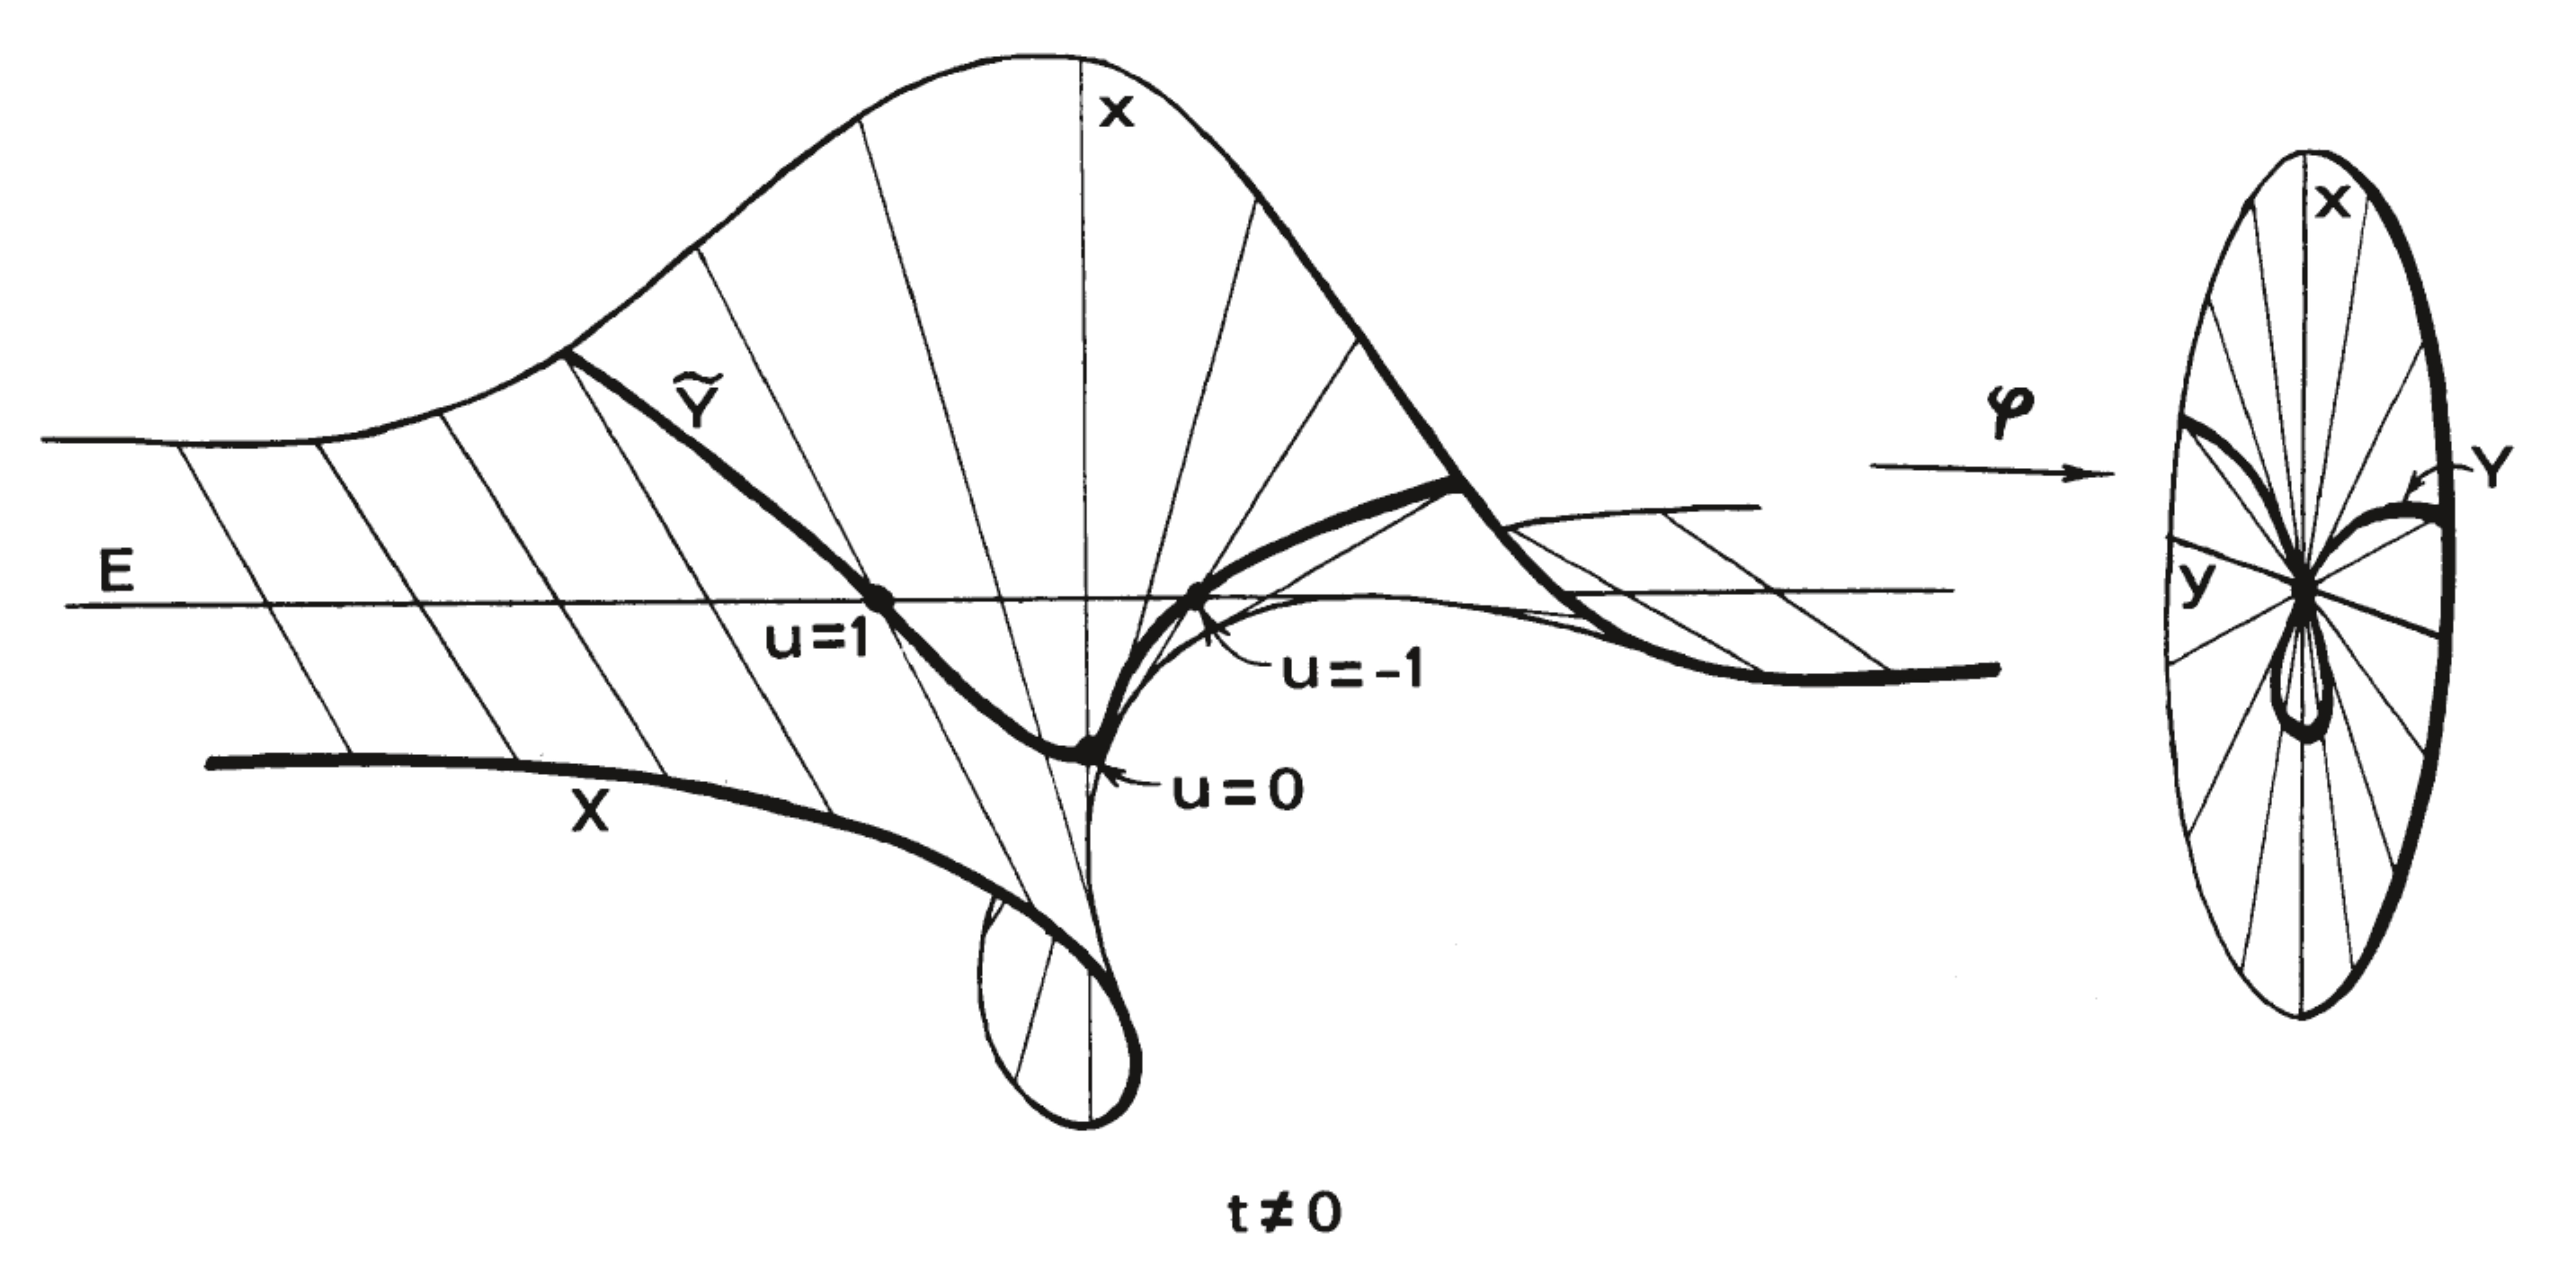
\includegraphics[width=0.8\columnwidth]{Figure3}\\
	Figure 3. 부풀림
	\end{center}
	
	
	%Definition
	\begin{definition}
	%
		\tn{$Y$가 $O$를 지나는 $\An$의 닫힌 부분대수다양체이면 \tb{$Y$의 점 $O$에서의 부풀림(blowing-up of $Y$ at the point $O$)}을
		$\tilde Y=\overline{(\ph^{-1}(Y-O))}$로 정의한다. 여기에서 $\ph:X\ra\An$은 위에 기술된 $\An$의 $O$에서의 부풀림이다.
		우리는 $\ph:X\ra\An$을 $\tilde Y$로 제한하여 얻어진 사상도 $\ph:\tilde Y\ta Y$로 표기한다.
		$\An$의 임의의 다른 점 $P$에서 부풀리기 위해서는 $P$를 $O$로 대응시키는 좌표계의 1차다항식에 의한 변환을 가하라.}
	%
	\end{definition}
	
	$\ph$가 $\tilde Y-\ph^{-1}(O)$와 $Y-O$ 간의 동형사상을 유도함을 기억해 두라.
	따라서 $\ph$는 $\tilde Y$에서 $Y$로의 쌍유리사상이다.
	또한 이러한 정의가 분명히 $Y$의 $\An$으로의 매장에 의존함을 기억해 두라.
	그러나 우리가 나중에 보일 것과 같이 사실 부풀림은 내재적이다. (II, 7.15.1)
	
	$Y$의 점에서의 부풀림의 효과는 $Y$를 $O$ 근처에서 $O$를 통과하는 다른 방향의 직선을 따라 `잡아 찢는' 것이다.
	우리는 이것을 예를 통해 소개하겠다.
	
	
	%Example 4.9.1
	\begin{example}
	%
		\tn{\\$Y$가 방정식 $y^2=x^2(x+1)$에 의해 주어진 평면 3차곡선이라 하자.
		우리는 $Y$를 $O$에서 부풀릴 것이다. (Fig. 3) $t,u$가 $\mb P^1$의 동차 좌표라 하자.
		그 경우 $\mb A^2$의 $O$에서의 부풀림 $X$는 $\mb A^2\times\mb P^1$ 내에서 방정식 $xu=ty$에 의해 정의된다.
		이는 점 $O$가 $O$를 통과하는 직선들의 기울기에 대응하는 $\mb P^1$로 대체된 것을 제외하면 $\mb A^2$처럼 보인다.
		우리는 이러한 $\mb P^1$을 \tb{예외곡선(exceptional curve)}이라 부르며 $E$로 표기할 것이다.\\
		우리는 $\mb A^2\times\mb P^1$에서 방정식 $y^2=x^2(x+1)$과 $xu=ty$를 고려하는 것으로 $Y$의 $X$에서의 전체 역상을 얻을 것이다.
		이제 $\mb P^1$은 열린집합 $t\ne 0$과 $u\ne 0$에 의해 덮이며 우리는 이들을 개별적으로 고려할 것이다.
		만약 $t\ne 0$이면 $t=1$이라 설정하고 $u$를 아핀 매개변수로 사용한다.
		그 경우 우리는 좌표계 $x,y,u$를 가지는 $\mb A^3$에서 다음 방정식을 얻는다.}
	%
		\begin{align*}
		y^2&=x^2(x+1)\\y&=xu
		\end{align*}
	%
		\tn{대입하면 우리는 $x^2u^2-x^2(x+1)=0$을 얻으며 이는 인수분해된다.
		그러므로 우리는 $x=0,y=0,$ 임의의 $u$에 의해 정의된 $E$와 $u^2=x+1,y=xu$에 의해 정의된 $\tilde Y$라는
		두 개의 기약 성분을 얻는다. $\tilde Y$가 $E$와 점 $u=\pm 1$에서 만남을 기억해 두라.
		이 점들은 $Y$의 $O$에서의 두 갈래의 기울기에 대응한다.\\
		마찬가지로 우리는 $x$축의 전체 역상이 $E$와 하나의 다른 기약 곡선으로 구성됨을 확인할 수 있으며
		우리는 이를 $x$축의 \tb{엄격한 변환(strict transform)}이라 한다.
		(이는 직선 $L=x$축에 대응하는 앞에서 기술한 곡선 $\bar L'$이다.)
		이러한 엄격한 변환은 점 $u=0$에서 $E$와 만난다. $\mb A^2\times\mb P^1$에서의 다른 열린집합 $u\ne 0$을 고려하면
		$y$축의 엄격한 변환이 $E$와 점 $t=0,u=1$에서 만남을 보일 수 있다.\\
		이러한 결론은 Figure 3에 요약되어 있다. 부풀림의 효과는 $O$를 통과하는 곡선의 가지들을 기울기에 따라 분리하는 것이다.
		만약 기울기가 다르다면 이들의 엄격한 변환은 $X$에서 만나지 않는다.
		대신 이들은 $E$와 서로 다른 기울기에 대응하는 점에서 만난다.}
	%
	\end{example}
	
	
	
	%Exercises
	\subsection*{Exercises (연습문제)}
	
	\begin{enumerate}[label=\tb{4.\arabic*.},itemindent=0mm,itemsep=2mm]
	\item 만약 $f$와 $g$가 대수다양체 $X$의 열린집합 $U$와 $V$ 상에서의 정칙 함수이며 $U\cap V$ 상에서 $f=g$이면
	$U$ 상에서 $f$이고 $V$ 상에서 $g$인 함수는 $U\cup V$ 상에서의 정칙 함수임을 보여라.
	만약 $f$가 $X$ 상에서의 \ti{유리}함수이면 $f$가 정칙 함수로 표현될 수 있도록 하는 $X$의 최대 열린 부분집합 $U$가 존재함을 보여라.
	우리는 $f$가 $U$의 점들에서 \tb{정의되었다(defined)}고 한다.
	\item 유리사상에 대한 동일한 문제. 만약 $\ph$가 $X$에서 $Y$로의 유리사상이면 $\ph$가 사상에 의해 표현되도록 하는
	최대 열린집합이 존재함을 보여라. 우리는 유리사상이 이러한 열린집합의 점들에서 \tb{정의되었다(defined)}고 한다.
	\item \begin{enumerate}[label=(\alph*)]
	\item $f$가 $f=x_1/x_0$에 의해 주어진 $\mb P^2$ 상에서의 유리함수라 하자.
	$f$가 정의된 점들의 집합을 찾고 대응하는 정칙 함수를 기술하라.
	\item 이제 이 함수를 $\mb P^2$에서 $\mb A^1$로의 유리사상으로 간주하자. $\mb A^1$을 $\mb P^1$에 매장하고
	$\ph:\mb P^2\ra\mb P^1$이 그 결과로 얻어진 유리사상이라 하자. $\ph$가 정의된 점들의 집합을 찾고 대응하는 사상을 기술하라.
	\end{enumerate}
	\item 대수다양체 $Y$가 \tb{유리(rational)}라는 것을 어떠한 $n$에 대하여 $\Pn$과 쌍유리동치인 것으로 정의하자.
	(또는 (4.5)에 의해 이와 동치로 $K(Y)$가 $k$의 순수히 초월적 확대인 것이다.)
	\begin{enumerate}[label=(\alph*)]
	\item $\mb P^2$에서의 임의의 원뿔곡선은 유리 곡선이다.
	\item 첨점을 가진 3차곡선 $y^2=x^3$은 유리 곡선이다.
	\item $Y$가 $\mb P^2$에서의 결절점을 가진 3차곡선 $y^2z=x^2(x+z)$라 하자. 점 $P=(0,0,1)$에서 직선 $z=0$으로의 사영 $\ph$%
	(Ex. 3.14)는 $Y$에서 $\mb P^1$으로의 쌍유리사상을 유도함을 보여라. 그러므로 $Y$는 유리 곡선이다.
	\end{enumerate}
	\item $\mb P^3$에서의 2차곡면 $Q:xy=zw$가 $\mb P^2$와 쌍유리이지만 $\mb P^2$와 동형은 아님을 보여라. (cf. Ex. 2.15)
	\item \tb{평면 Cremona 변환.} $\mb P^2$에서 자신으로의 쌍유리사상은
	\tb{평면 Cremona 변환(plane Cremona transformation)}이라 불린다.
	\tb{2차 변환(quadratic transformation)}이라 불리는 예를 제시하겠다. 이는 $a_0,a_1,a_2$ 중 두 개가 0이지는 않은 경우
	$(a_0,a_1,a_2)\ra(a_1a_2,a_0a_2,a_0a_1)$에 의해 주어진 유리사상 $\ph:\mb P^2\ra\mb P^2$이다.
	\begin{enumerate}[label=(\alph*)]
	\item $\ph$가 쌍유리이며 스스로의 역임을 보여라.
	\item $\ph:U\ra V$가 동형사상이도록 하는 열린집합 $U,V\bseq\mb P^2$를 찾아라.
	\item $\ph$와 $\ph^{-1}$이 정의된 열린집합을 찾고 대응되는 사상을 기술하라. (V, 4.2.3)도 참조하라.
	\end{enumerate}
	\item $X$와 $Y$가 대수다양체라 하자. 점 $P\in X$와 $Q\in Y$가 존재하여
	국소환 $\mc O_{P,X}$와 $\mc O_{Q,Y}$가 $k$-대수로서 동형이라 하자.
	그 경우 열린집합 $P\in U\bseq X$와 $Q\in V\bseq Y$와 $P$를 $Q$로 대응시키는 $U$에서 $V$로의 동형사상이 존재한다.
	\item \begin{enumerate}[label=(\alph*)]
	\item $k$ 상에서의 임의의 양수 차원 대수다양체가 $k$와 동일한 기수를 가짐을 보여라.
	[Hint: 먼저 $\An$과 $\Pn$에 대하여 보여라. 그 후 임의의 $X$에 대하여 차원 $n$에 대한 귀납법을 사용하라.
	(4.9)를 사용하여 $X$가 초곡면 $H\bseq\mb P^{n+1}$과 쌍유리이도록 하라. (Ex. 3.7)을 사용하여
	$H$에 속하지 않은 한 점에서 $\Pn$으로의 $H$의 사영이 유한 개 점을 한 점으로 대응시키며 전사임을 보여라.]
	\item $k$ 상에서의 임의의 두 \ti{곡선}이 위상동형임을 연역하라. (cf. Ex. 3.1)
	\end{enumerate}
	\item $X$가 $\Pn$에서의 $r$차원 사영 대수다양체이며 $n\ge r+2$라 하자.
	적절한 $P\notin X$와 선형 대수다양체 $\mb P^{n-1}\bs\Pn$의 선택에 대하여 $P$에서 $\mb P^{n-1}$로의 사영(Ex. 3.14)이
	$X$에서 그 상 $X'\bseq\mb P^{n-1}$으로의 \ti{쌍유리사상}인 사상을 유도함을 보여라.
	(4.6A), (4.7A), (4.8A)가 필요할 것이다. 이는 특히 (4.9)의 쌍유리사상이 이러한 유한 번의 사영을 통해 얻어질 수 있음을 보여준다.
	\item $Y$가 $\mb A^2$에서의 첨점을 가진 3차곡선 $y^2=x^3$이라 하자.
	점 $O=(0,0)$을 부풀리고 $E$가 예외곡선이며 $\tilde Y$가 $Y$의 엄격한 변환이라 하자.
	$E$가 $\tilde Y$와 한 점에서 만나며 $\tilde Y\cong\mb A^1$임을 보여라.
	이 경우 사상 $\ph:\tilde Y\ra Y$가 전단사 쌍연속이지만 동형사상은 아니다.
	\end{enumerate}
	
	
	
	%Section 5
	\section{Nonsingular Varieties (비특이 대수다양체)}
	%
	대수기하학에서 비특이 대수다양체의 개념은 위상수학에서 다양체의 개념에 대응된다.
	예를 들어 복소수체 상에서 비특이 대수다양체들은 `표준'위상이 복소다양체인 것들이다.
	그러므로 가장 자연스러운 (그리고 역사적으로 먼저 등장했던) 비특이성의 정의는
	대수다양체를 정의하는 함수들의 도함수를 이용하는 것이다:
	
	
	%Definition
	\begin{definition}
	%
		\tn{$Y\bseq\An$이 아핀 대수다양체이며 $f_1,\ldots,f_t\in A=k[x_1,\ldots,x_n]$이 $Y$의 아이디얼의 생성집합이라 하자.
		$Y$가 \tb{점 $P\in Y$에서 비특이(nonsingular at a point $P\in Y$)}임은
		행렬 $\|(\pa f_i/\pa x_j)(P)\|$의 계수가 $n-r$인 것이다. (여기에서 $r$은 $Y$의 차원이다.)
		$Y$가 \tb{비특이(nonsingular)}임은 모든 점에서 비특이인 것이다.}
	%
	\end{definition}
	
	몇 가지를 첨언하겠다. 먼저 다항식의 어떠한 한 변수에 대한 편도함수의 개념은 임의의 체 상에서 유효하다.
	(통상적인 미분 규칙을 적용하면 된다.) 그러므로 극한 과정이 필요하지 않다. 그러나 표수 $p>0$의 경우 웃긴 일이 발생할 수 있다.
	예를 들어 $f(x)=x^p$이면 ($k$에서 $p=0$이므로) $df/dx=px^{p-1}=0$이다.
	모든 경우 만약 $f\in A$가 다항식이면 각각의 $i$에 대하여 $\pa f/\pa x_i$는 다항식이다.
	행렬 $\|(\pa f_i/\pa x_j)(P)\|$는 $P$에서의 \tb{Jacobi 행렬(Jacobian matrix)}이라 불린다.
	이러한 비특이성의 정의가 $Y$의 아이디얼의 생성집합의 선택에 독립적임을 간단히 보일 수 있다.
	
	우리의 정의의 한 가지 문제점은 $Y$의 아핀 공간으로의 매장에 의존한다는 것이다.
	그러나 기본적인 문헌 Zariski [1]에서 비특이성은 국소환에 의해 내재적으로 기술될 수 있음이 밝혀졌다.
	우리의 경우 그 결과는 다음과 같다.
	
	%Definition
	\begin{definition}
	%
		\tn{$A$가 Noether 국소환이며 극대 아이디얼 $\mf m$과 잉여류체 $k=A/\mf m$을 가진다 하자.
		$A$가 \tb{정칙 국소환(regular local ring)}이라는 것의 정의는 $\dim[k]\mf m/\mf m^2=\dim A$인 것이다.}
	%
	\end{definition}
	
	
	%Theorem 5.1
	\begin{theorem}
	%
		\tn{$Y\bseq\An$이 아핀 대수다양체라 하자. $P\in Y$가 점이라 하자.
		그 경우 $Y$가 $P$에서 비특이일 필요충분조건은 국소환 $\mc O_{P,Y}$가 정칙 국소환인 것이다.\\\\
	%
		\pf $P$가 $\An$에서의 점 $(a_1,\ldots,a_n)$이며 $\mf a_P=(x_1-a_1,\ldots,x_n-a_n)$이
		대응하는 $A=k[x_1,\ldots,x_n]$에서의 극대 아이디얼이라 하자.
		선형 사상 $\ta:A\ra k^n$을 임의의 $f\in A$에 대하여 다음과 같이 정의한다.}
	%
		$$\ta(f)=\Braket{\pdif f{x_1}(P),\ldots,\pdif f{x_n}(P)}$$
	%
		\tn{이제 $i=1,\ldots,n$에 대하여 $\ta(x_i-a_i)$들이 $k^n$의 기저를 형성하며 $\ta(\mf a_P^2)=0$임은 명백하다.
		그러므로 $\ta$는 동형사상 $\ta':\mf a_P/\mf a_P^2\ra k^n$을 유도한다.\\
		이제 $\mf b$가 $Y$의 $A$에서의 아이디얼이며 $f_1,\ldots,f_t$가 $\mf b$의 생성집합이라 하자.
		그 경우 Jacobi 행렬 $J=\|(\pa f_i/\pa x_j)(P)\|$의 계수는 $k^n$의 부분공간으로서 $\ta(\mf b)$의 차원이다.
		동형사상 $\ta'$을 이용하면 이는 $\mf a_P/\mf a_P^2$의 부분공간 $(\mf b+\mf a_P^2)/\mf a_P^2$의 차원과 동일하다.
		반면에 $Y$ 상에서의 $P$의 국소환 $\mc O_P$는 $A$를 $\mf b$로 나누고 극대 아이디얼 $\mf a_P$에서 국소화하여 얻어진다.
		그러므로 만약 $\mf m$이 $\mc O_P$의 극대 아이디얼이면 다음이 성립한다.}
	%
		$$\mf m/\mf m^2\cong\mf a_P/(\mf b+\mf a_P^2)$$
	%
		\tn{벡터 공간의 차원을 계산하면 $\dim\mf m/\mf m^2+\rank J=n$을 얻는다.\\
		이제 $\dim Y=t$이라 하자. 그 경우 $\mc O_P$는 $r$차원의 국소환이며 (3.2)
		따라서 $\mc O_P$가 정칙일 필요충분조건은 $\dim[k]\mf m/\mf m^2=r$인 것이다.
		그러나 이는 $\rank J=n-r$임과 동치이며 이는 $P$가 $Y$의 비특이점인 것과 동치이다.}
	%
	\end{theorem}
	
	\ti{Note}. 나중에 우리는 $Y$ 상에서의 미분 형식들의 층에 의한 비특이점의 다른 특성화를 제시할 것이다. (II, 8.15)\\
	
	이제 우리는 비특이성의 개념이 내재적임을 알게 되었으므로 정의를 임의의 대수다양체로 확장할 수 있다.
	
	
	%Definition
	\begin{definition}
	%
		\tn{$Y$가 임의의 대수다양체라 하자. $Y$가 점 $P\in Y$에서 \tb{비특이(nonsingular)}라는 것의 정의는
		국소환 $\mc O_{P,Y}$가 정칙 국소환인 것이다. $Y$가 \tb{비특이(nonsingular)}라는 것의 정의는 모든 점에서 비특이인 것이다.
		$Y$가 \tb{특이(singular)}라는 것의 정의는 비특이가 아닌 것이다.}
	%
	\end{definition}
	
	우리의 다음 목표는 대수다양체의 대부분의 점들이 비특이임을 보이는 것이다. 이를 위해서는 대수학적 예비지식이 필요하다.
	
	
	%Proposition 5.2A
	\begin{propositiona}
	%
		\tn{\\만약 $A$가 Noether 국소환이며 극대 아이디얼 $\mf m$과 잉여류체 $k$를 가지면
		$\dim[k]\mf m/\mf m^2\ge\dim A$이다.\\\\
	%
		\pf Atiyah-Macdonald [1, Cor. 11.15, p.121] 또는 Matsumura [2, p. 78]}
	%
	\end{propositiona}
	
	
	%Theorem 5.3
	\begin{theorem}
	%
		\tn{\\$Y$가 대수다양체라 하자. $Y$의 특이점들의 집합 $\Sing Y$는 $Y$의 닫힌 진부분집합이다.\\\\
	%
		\pf (II, 8.16을 참조하라.) 먼저 우리는 $\Sing Y$가 닫힌 부분집합임을 보일 것이다.
		$Y$의 어떠한 열린 덮개 $Y=\bigcup Y_i$에 대하여 각각의 $i$에 대하여 $\Sing Y_i$가 닫혀 있음을 보이면 충분하다.
		따라서 (4.3)에 의해 우리는 $Y$가 아핀이라 가정할 수 있다. (5.2)와 (5.1)의 증명에 의해
		우리는 Jacobi 행렬의 계수가 항상 $n-r$ 이하임을 알고 있다. 따라서 특이점들의 집합은 계수가 $n-r$ 미만인 곳이다.
		그러므로 $\Sing Y$는 $I(Y)$와 행렬 $\|\pa f_i/\pa x_j\|$의 모든 $(n-r)\times(n-r)$ 부분행렬들의 행렬식들에 의해
		생성된 아이디얼에 의해 정의된 대수적 집합이다. 따라서 $\Sing Y$는 닫혀 있다.\\
		$\Sing Y$가 $Y$의 진부분집합임을 보이기 위해 먼저 (4.9)를 적용하여 $Y$가 $\Pn$에서의 초곡면과 쌍유리임을 얻는다.
		쌍유리 대수다양체들은 동형인 열린집합들을 가지므로 초곡면의 경우로 문제를 줄일 수 있다.
		$Y$의 임의의 아핀 열린 부분집합을 고려하면 충분하며
		따라서 우리는 $Y$가 하나의 기약다항식 $f(x_1,\ldots,x_n)=0$에 의해 정의된 $\An$에서의 초곡면이라 가정할 것이다.\\
		이제 $\Sing Y$는 $i=1,\ldots,n$에 대하여 $(\pa f/\pa x_i)(P)=0$을 만족시키는 점 $P\in Y$들의 집합이다.
		만약 $\Sing Y=Y$이면 함수 $\pa f/\pa x_i$들이 $Y$ 상에서 항등적으로 0이며
		따라서 각각의 $i$에 대하여 $\pa f/\pa x_i\in I(Y)$이다. 그러나 $I(Y)$는 $f$에 의해 생성된 주 아이디얼이며
		각각의 $i$에 대하여 $\deg(\pa f/\pa x_i)\le\deg f-1$이므로 각각의 $i$에 대하여 $\pa f/\pa x_i=0$이어야 한다.\\
		표수 0의 경우 만약 $x_i$가 $f$에서 나타난다면 $\pa f/\pa x_i\ne 0$이므로 이는 불가능하다.
		따라서 $\Char k=p>0$이어야 한다. 이 경우 $\pa f/\pa x_i=0$이라는 사실은 $f$가 $x_i^p$의 다항식임을 함의한다.
		이는 각각의 $i$에 대하여 참이며 따라서 계수의 $p$제곱근을 취하면 ($k$가 대수적으로 닫혀 있으므로 이는 가능하다)
		$f=g^p$를 만족시키는 다항식 $g(x_1,\ldots,x_n)$을 얻는다. 그러나 이는 $f$가 기약이라는 전제조건에 모순이며
		따라서 $\Sing Y<Y$라 결론지을 수 있다.}
	%
		\qed
	%
	\end{theorem}
	
	
	
	%Subsection
	\subsection*{Completion (완비화)}
	%
	특이점을 국소적으로 분석하기 위해 우리는 이제 완비화의 기법을 기술할 것이다.
	$A$가 극대 아이디얼 $\mf m$을 가지는 국소환이라 하자.
	$\mf m$의 멱들은 $A$ 상에 \tb{$\mf m$진 위상($\mf m$-adic topology)}이라 불리는 위상을 정의한다.
	이러한 위상에 대하여 완비화하면 $\hat A$로 표기되는 $A$의 \tb{완비화(completion)}를 얻는다.
	이와 동치로 우리는 $\hat A$를 역극한 $\ds\lim_\longleftarrow A/\mf m^n$으로 정의할 수 있다.
	완비화에 관한 일반적인 정보를 위해서는
	Atiyah-Macdonald [1, Ch. 10], Matsumura [2, Ch. 9], 또는 Zariski-Samuel [1, Vol. 2, Ch. VIII]를 참조하라.
	
	완비화의 대수기하학에서의 중요성은 대수다양체 $X$ 상의 점 $P$에서의 국소환의 완비화 $\hO P$에서
	$X$의 $P$ 근처에서의 매우 국소적인 거동을 연구할 수 있다는 것이다.
	우리는 점 $P\in X$와 $Q\in Y$가 동형인 국소환을 가지면 $P$와 $Q$가 동형인 근방을 가지며 따라서 $X$와 $Y$가 쌍유리임을 보였다.
	(Ex. 4.7) 그러므로 통상적인 국소환 $\mc O_P$는 $X$의 거의 전체에 관한 정보를 포함한다.
	그러나 완비화 $\hO P$는 (앞으로 보게 될 것과 같이) 위상수학이나 미분기하학에서의 `국소'의 의미에 관한
	우리의 직관과 가까운 훨씬 더 국소적인 정보를 포함한다.
	
	우리는 완비화의 몇 가지 대수적 성질을 상기하고 예시를 제시하겠다.
	
	
	%Theorem 5.4A
	\begin{theorema}
	%
		\tn{\\$A$가 Noether 국소환이며 극대 아이디얼 $\mf m$을 가지고 $\hat A$가 그 완비화라 하자.
	%
		\begin{enumerate}[label=(\alph*)]
		\item $\hat A$는 극대 아이디얼 $\hat{\mf m}=\mf m\hat A$를 가지는 국소환이며
		자연스러운 단사 준동형사상 $A\ra\hat A$가 존재한다.
		\item 만약 $M$이 유한생성 $A$-모듈이면 그 $\mf m$진 위상에 대한 완비화 $\hat M$은 $M\otimes_A\hat A$와 동형이다.
		\item $\dim A=\dim\hat A$
		\item $A$가 정칙일 필요충분조건은 $\hat A$가 정칙인 것이다.
		\end{enumerate}}
	%
		\tn{\\\pf Atiyah-Macdonald [1, Ch. 10, 11] 또는 Zariski-Samuel [1, vol. 2, Ch. VIII]를 참조하라.}
	%
	\end{theorema}
	
	
	%Theorem 5.5A
	\begin{theorema}[Cohen Structure Theorem (Cohen 구조 정리)]
	%
		\tn{\\만약 $A$가 $n$차원 완비 정칙 국소환이며 어떠한 체를 포함하면
		$A\cong k[[x_1,\ldots,x_n]]$($A$의 잉여류체 $k$ 상에서의 형식적 멱급수환)이다.\\\\
	%
		\pf Matsumura [2, Cor. 2, p.206] 또는 Zariski-Samuel [1, vol. 2, Cor., p. 307]}
	%
	\end{theorema}
	
	
	%Definition
	\begin{definition}
	%
		\tn{두 점 $P\in X$와 $Q\in Y$가 \tb{해석적 동형(analayically isomorphic)}이라는 것의 정의는
		$k$-대수 동형사상 $\hO P\cong\hO Q$가 존재하는 것이다.}
	%
	\end{definition}
	
	
	\setcounter{theorem}{6}
	%Example 5.6.1
	\begin{example}
	%
		\tn{\\만약 $P\in X$와 $Q\in Y$가 해석적 동형이면 $\dim X=\dim Y$이다.
		이는 (5.4A)와 대수다양체 상의 임의의 점에서의 국소환은 대수다양체와 동일한 차원을 가진다는 사실에서 따라온다. (Ex. 3.12)}
	%
	\end{example}
	
	
	%Example 5.6.2
	\begin{example}
	%
		\tn{\\만약 $P\in X$와 $Q\in Y$가 같은 차원의 대수다양체 상의 비특이점들이면 $P$와 $Q$는 해석적 동형이다.
		이는 (5.4A)와 (5.5A)로부터 따라온다.
		이 예는 동일한 차원의 두 (위상, 미분, 복소)다양체가 국소적으로 동형이라는 사실의 대수적 유사체이다.}
	%
	\end{example}
	
	
	%Example 5.6.3
	\begin{example}
	%
		\tn{\\$X$가 방정식 $y^2=x^2(x+1)$에 의해 주어진 결절점을 가지는 평면 3차곡선이라 하자.
		$Y$가 $xy=0$에 의해 정의된 $\mb A^2$에서의 대수적 집합이라 하자.
		우리는 $X$ 상에서의 점 $O=(0,0)$이 $Y$ 상에서의 점 $O$와 대수적으로 동형임을 보일 것이다.
		(우리가 아직 기약 대수적 집합 상에서의 점의 국소환에 관한 일반적인 이론을 개발하지 않았으므로
		우리는 ad hoc 정의 $\mc O_{O,Y}=(k[x,y]/(xy))_{(x,y)}$를 사용할 것이다. 그러므로 $\hO{O,Y}\cong k[[x,y]]/(xy)$이다.)
		이러한 예는 $O$ 근처에서 $X$가 두 선이 교차하는 것처럼 보인다는 기하학적 사실에 대응된다.\\
		이 결과를 증명하기 위해 $k[[x,y]]/(y^2-x^2-x^3)$과 동형인 완비화 $\hO{O,X}$를 고려하자.
		핵심은 방정식의 주요 항 $y^2-x^2$가 서로 다른 두 인수 $y+x$와 $y-x$로 인수분해된다는 것이다.
		($\Char k\ne 2$라 가정한다.) $k[[x,y]]$에 속한 다음과 같은 두 형식적 멱급수가 존재하여 $g_i,h_i$가 동차 $i$차이며
		$y^2-x^2-x^3=gh$임을 주장하겠다.}
	%
		\begin{align*}
		g&=y+x+g_2+g_3+\cdots\\
		h&=y-x+h_2+h_3+\cdots
		\end{align*}
	%
		\tn{$g$와 $h$를 단계적으로 구축하겠다. $g_2$와 $h_2$를 결정하기 위해 다음이 필요하다.}
	%
		$$(y-x)g_2+(y+x)h_2=-x^3$$
	%
		\tn{$y-x$와 $y+x$가 $k[[x,y]]$의 극대 아이디얼을 생성하므로 이는 가능하다. $g_3$과 $h_3$을 결정하기 위해 다음이 필요하다.}
	%
		$$(y-x)g_3+(y+x)h_3=-g_2h_2$$
	%
		\tn{이는 다시 가능하며 이러한 방법으로 반복한다.\\
		그러므로 $\hO{O,X}=k[[x,y]]/(gh)$이다. $g$와 $h$가 선형 독립인 1차항으로 시작하므로 $k[[x,y]]$의 자기동형사상이 존재하여
		$g$와 $h$를 각각 $x$와 $y$로 대응시킨다. 이는 요구된 것과 같이 $\hO{O,X}\cong k[[x,y]]/(xy)$임을 보여준다.\\
		이 예에서 $\mc O_{O,X}$가 정역이지만 그 완비화는 정역이 아님을 기억해 두라.}
	%
	\end{example}
	
	아래의 (Ex. 5.15)에서 사용될 대수적 결과를 여기에 기술해 놓겠다.
	
	
	%Theorem 5.7A
	\begin{theorema}[Elimination Theory (소멸 이론)]
	%
		\tn{\\$f_1,\ldots,f_r$이 $x_0,\ldots,x_n$에 대한 동차다항식들이며 미정계수 $a_{ij}$들을 가진다 하자.
		그 경우 $a_{ij}$에 대한 정수계수 다항식들의 집합 $g_1,\ldots,g_t$가 존재하여
		각각의 $f_i$의 계수들에 대하여 개별적으로 동차이고 다음 성질을 가진다:
		임의의 체 $k$와 임의의 특정한 값 $a_{ij}\in k$들의 집합에 대하여
		$f_i$들이 $(0,\ldots,0)$ 이외의 공통영점을 가질 필요충분조건은 $a_{ij}$들이 다항식 $g_j$들의 공통영점인 것이다.\\\\
	%
		\pf Van der Waerden [1, Vol. II, \S 80, p. 8]}
	%
	\end{theorema}
	
	
	%Exercises
	\subsection*{Exercises (연습문제)}
	
	\begin{enumerate}[label=\tb{5.\arabic*.},itemindent=0mm,itemsep=2mm]
	\item $\mb A^2$에서의 다음 곡선들의 특이점의 위치를 찾고 형태를 그려라. ($\Char k\ne 2$라 가정하라.)
	각각의 방정식에 대응하는 곡선은 Figure 4에서 어떤 것인가?
	\begin{enumerate}[label=(\alph*)]
	\item $x^2=x^4+y^4$
	\item $xy=x^6+y^6$
	\item $x^3=y^2+x^4+y^4$
	\item $x^2y+xy^2=x^4+y^4$
	\end{enumerate}
	\end{enumerate}
	%
	%Figure 4
	\begin{center}
	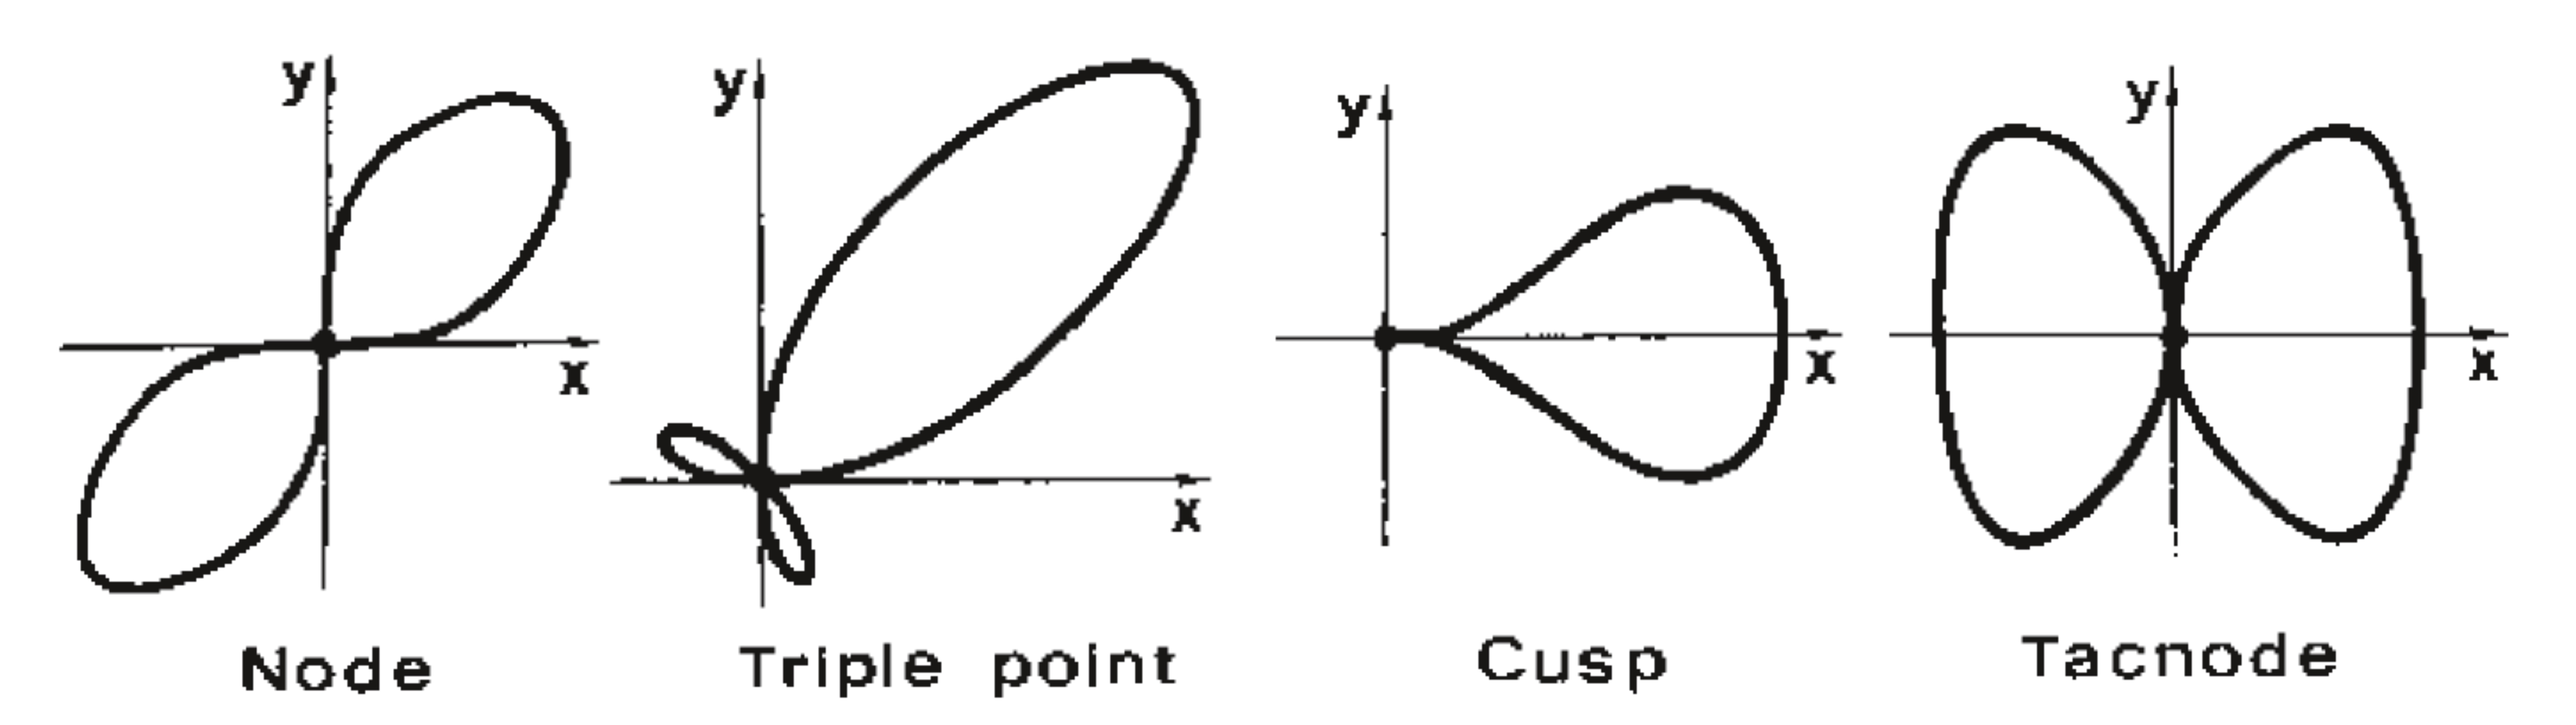
\includegraphics[width=0.8\columnwidth]{Figure4}\\
	Figure 4. 평면 곡선의 특이점
	\end{center}
	%
	\begin{enumerate}[label=\tb{5.\arabic*.},itemindent=0mm,itemsep=2mm]
	\setcounter{enumi}{1}
	\item 다음과 같은 $\mb A^3$에서의 곡면들의 특이점의 위치를 찾고 특이점을 기술하라. ($\Char k\ne 2$라 가정하라.)
	각각의 방정식에 대응하는 곡선은 Figure 5에서 어떤 것인가?
	\begin{enumerate}[label=(\alph*)]
	\item $xy^2=z^2$
	\item $x^2+y^2=z^2$
	\item $xy+x^3+y^3=0$
	\end{enumerate}
	\end{enumerate}
	%
	%Figure 5
	\begin{center}
	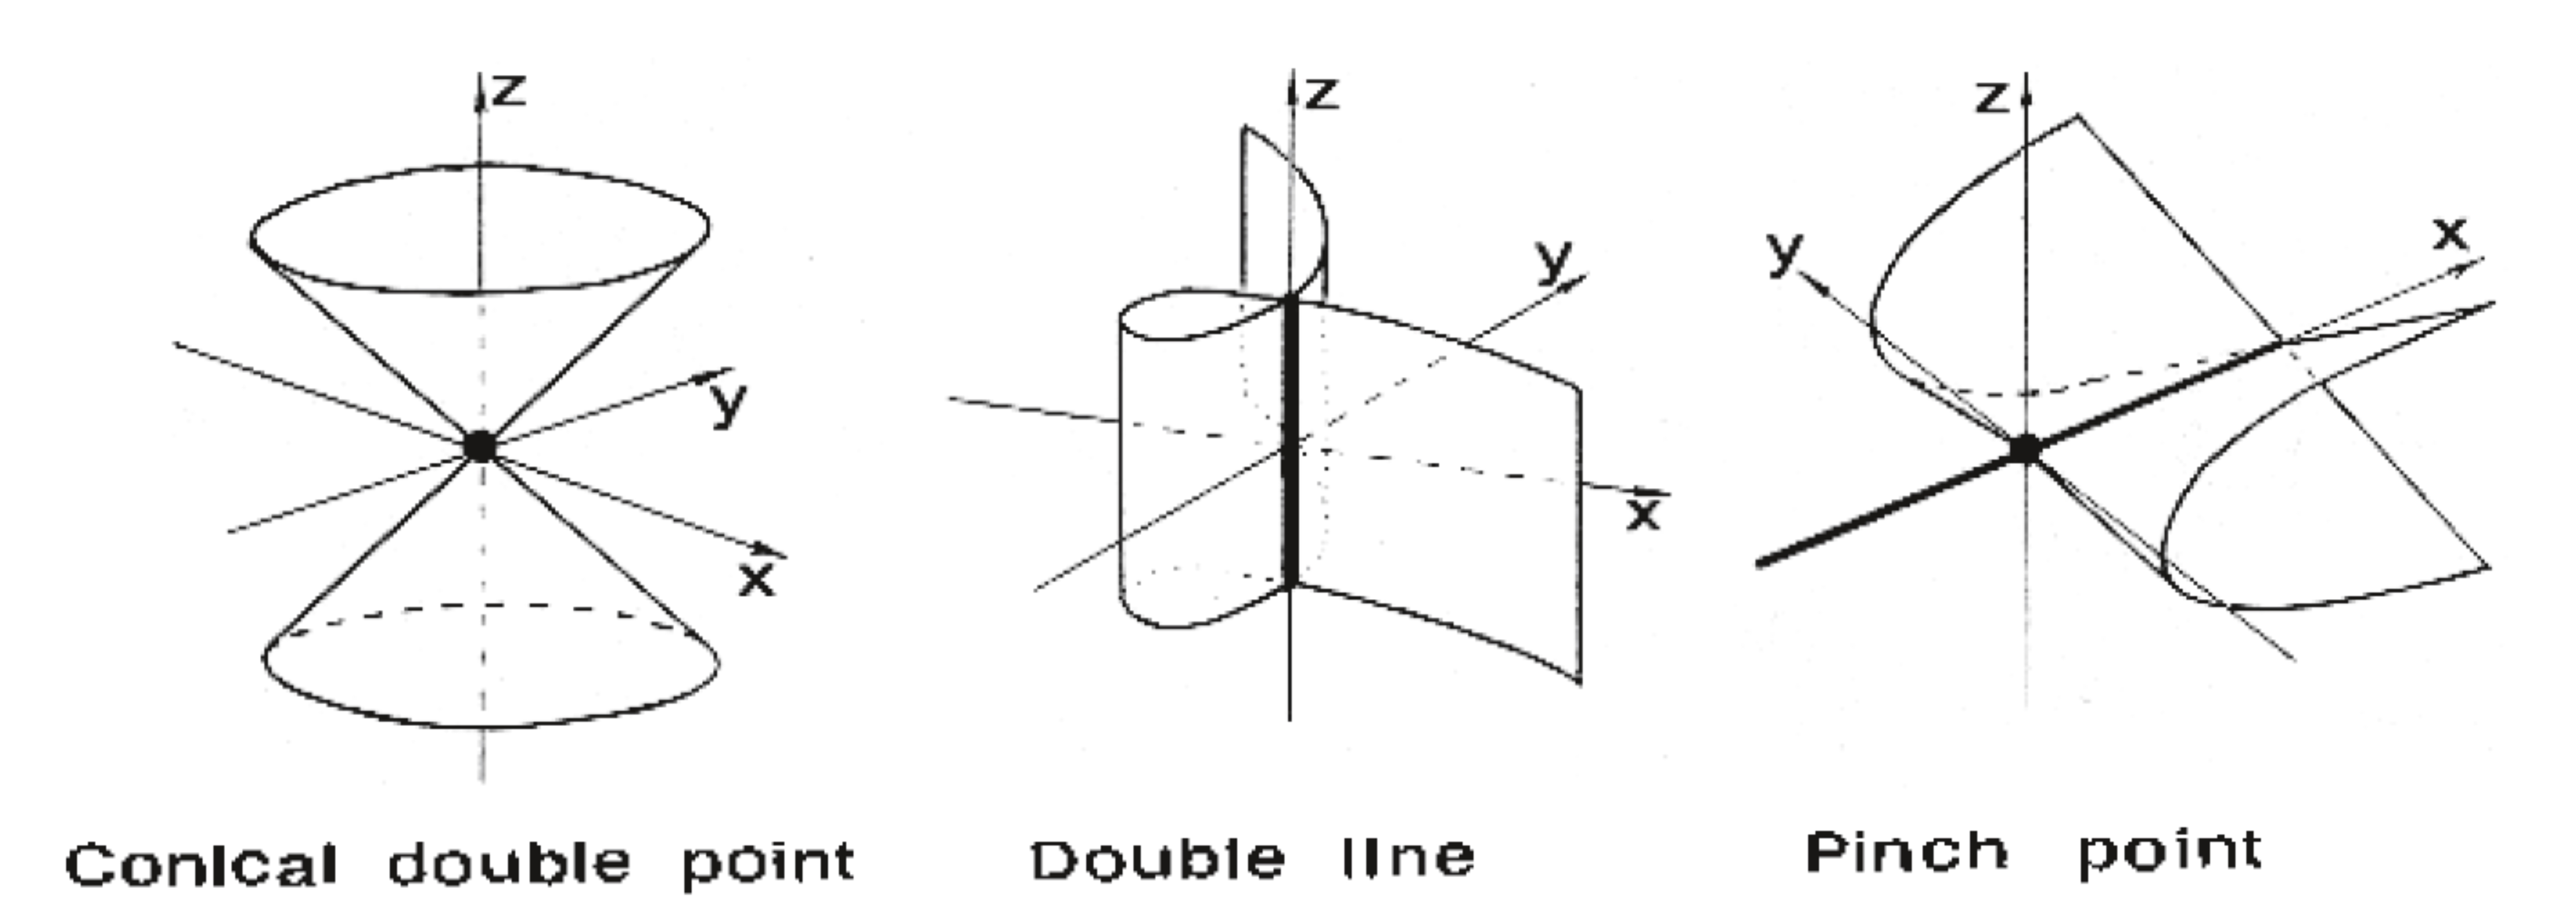
\includegraphics[width=0.8\columnwidth]{Figure5}\\
	Figure 5. 곡면 특이점
	\end{center}
	%
	\begin{enumerate}[label=\tb{5.\arabic*.},itemindent=0mm,itemsep=2mm]
	\setcounter{enumi}{2}
	\item \tb{중복도.} $Y\bseq\mb A^2$가 방정식 $f(x,y)=0$에 의해 정의된 곡선이라 하자. $P=(a,b)$가 $\mb A^2$의 점이라 하자.
	좌표계를 1차다항식에 의해 변환하여 $P$가 점 $(0,0)$이 되도록 하자.
	그 후 $f$를 $x$와 $y$에 대한 $i$차 동차다항식 $f_i$들의 합 $f=f_0+f_1+\cdots+f_d$로 표현하자.
	$P$의 $Y$ 상에서의 \tb{중복도(multiplicity)}를 $f_r\ne 0$이도록 하는 최소 $r$로 정의하고 $\mu_P(T)$로 표기하자.
	($P\in Y\Lra\mu_P(Y)>0$임을 기억해 두라.) $f_r$의 선형 인수들은 $P$에서의 \tb{접선방향(tangent direction)}들이라 불린다.
	\begin{enumerate}[label=(\alph*)]
	\item $\mu_P(T)=1\Lra P$가 $Y$의 비특이점인 것임을 보여라.
	\item 위의 (Ex. 5.1)에 있는 각각의 특이점들의 중복도를 찾아라.
	\end{enumerate}
	\item \tb{교차 중복도.} 만약 $Y,Z\bseq\mb A^2$가 서로 다른 두 곡선이며 방정식 $f=0,g=0$에 의해 주어지고 만약 $P\in Y\cap Z$이면
	$Y$와 $Z$의 $P$에서의 \tb{교차 중복도(intersection multiplicity)} $(Y\cdot Z)_P$를
	$\mc O_P$-모듈 $\mc O_P/(f,g)$의 길이로 정의한다.
	\begin{enumerate}[label=(\alph*)]
	\item $(Y\cdot Z)_P$가 유한하며 $(Y\cdot Z)_P\ge\mu_P(Y)\cdot\nu_P(Z)$임을 보여라.
	\item 만약 $P\in Y$이면 $P$를 통과하는 거의 모든(i.e. 유한 개를 제외한 모든) 직선 $L$에 대하여 $(L\cdot Y)_P=\mu_P(Y)$임을 보여라.
	\item 만약 $Y$가 $\mb P^2$에서의 $d$차곡선이며 $L$이 $\mb P^2$에서의 직선이고 $L\ne Y$이면 $(L\cdot Y)=d$임을 보여라.
	여기에서 $(L\cdot Y)=\sum(L\cdot Y)_P$(모든 점 $P\in L\cap Y$에 대한 합)로 정의하며
	$(L\cdot Y)_P$는 $\mb P^2$의 적절한 아핀 덮개를 이용하여 정의된다.
	\end{enumerate}
	\item 모든 차수 $d>0$과 $p=0$ 또는 임의의 소수 $p$에 대하여 표수 $p$의 체 $k$ 상에서의
	$\mb P^2$에서의 비특이 $d$차곡선의 방정식을 제시하라.
	\item \tb{곡선 특이점의 부풀림.}
	\begin{enumerate}[label=(\alph*)]
	\item $Y$가 (Ex. 5.1)의 첨점 또는 결절점을 가지는 곡선이라 하자. $Y$를 $O=(0,0)$에서 부풀려 얻어진 곡선 $\tilde Y$는 비특이이다.
	(cf. (4.9.1)과 (Ex. 4.10))
	\item \tb{결절점(node)}(또는 \tb{통상2중점(ordinary double point)})을 서로 다른 접선방향(Ex. 5.3)들을 가지는
	평면 곡선의 2중점(i.e. 중복도 2의 점)으로 정의한다.
	만약 $P$가 평면 곡선 $Y$ 상에서의 결절점이면 $\ph^{-1}(P)$가 부풀려진 곡선 $\tilde Y$ 상에서의
	서로 다른 두 개의 비특이점들로 구성됨을 보여라. 우리는 `$P$를 부풀리는 것이 $P$에서의 특이점을 해소한다'고 말한다.
	\item $P\in Y$가 (Ex. 5.1)의 접촉절점이라 하자.
	만약 $\ph:\tilde Y\ra Y$가 $P$에서의 부풀림이면 $\ph^{-1}(P)$가 ($\Char k\ne 2$인 경우) 결절점임을 보여라.
	(b)를 이용하면 우리는 접촉절점이 2회의 순차적인 부풀림에 의해 해소될 수 있음을 알 수 있다.
	\item $Y$가 평면 곡선 $y^3=x^5$라 하자. 이는 $O$에서 `고차 첨점'을 가진다.
	$O$가 3중점임을 보여라; $O$를 부풀리는 것은 2중점을 제공한다. (어떠한 형태의 2중점인가?) 한 번 더 부풀리면 특이점이 해소된다.
	\end{enumerate}
	\ti{Note}: 우리는 나중에 (V, 3.8) 평면 곡선의 임의의 특이점이 유한 회의 순차적인 부풀림에 의해 해소될 수 있음을 보일 것이다.
	\item $Y\bseq\mb P^2$가 방정식 $f(x,y,z)=0$에 의해 정의된 1차 초과의 비특이 평면 곡선이라 하자.
	$X\bseq\mb A^3$이 $f$에 의해 정의된 아핀 대수다양체라 하자. (이는 $Y$ 상에서의 뿔이다; (Ex. 2.10)을 참조하라.)
	$P$가 뿔의 \tb{꼭짓점(vertex)}인 점 $(0,0,0)$이라 하자. $\ph:\tilde X\ra X$가 $X$의 $P$에서의 부풀림이라 하자.
	\begin{enumerate}[label=(\alph*)]
	\item $X$가 하나의 특이점 $P$만을 가짐을 보여라.
	\item $\tilde X$가 비특이임을 보여라. (이를 아핀 열린집합들로 덮어라.)
	\item $\ph^{-1}(P)$가 $Y$와 동형임을 보여라.
	\end{enumerate}
	\item $Y\bseq\mb P^n$이 $r$차원 사영 대수다양체라 하자.
	$f_1,\ldots,f_t\in S=k[x_0,\ldots,x_n]$이 $Y$의 아이디얼을 생성하는 동차다항식들이라 하자.
	$P\in Y$가 동차 좌표 $P=(a_0,\ldots,a_n)$을 가지는 점이라 하자.
	$P$가 $Y$ 상에서 비특이일 필요충분조건은 행렬 $\|(\pa f_i/\pa x_j)(a_0,\ldots,a_n)\|$의 계수가 $n-r$인 것임을 보여라.
	[Hint: (a) 이러한 계수가 $P$에 대하여 선택된 동차 좌표계에 독립적임을 보여라.
	(b) $P$를 포함하는 아핀 열린집합 $U_i\bseq\Pn$으로 보내고 아핀 Jacobi 행렬을 사용하라.
	(c) $f$가 $d$차 동차이면 $\sum x_i(\pa f/\pa x_i)=d\cdot f$라는 Euler 보조정리가 필요할 것이다.]
	\item $f\in k[x,y,z]$가 동차다항식이고 $Y=Z(f)\bseq\mb P^2$가 $f$에 의해 정의된 대수적 집합이며
	모든 $P\in Y$에 대하여 $(\pa f/\pa x)(P),(\pa f/\pa y)(P),(\pa f/\pa z)(P)$ 중 적어도 하나가 0이라 하자.
	$f$가 기약(이며 따라서 $Y$가 비특이 대수다양체)임을 보여라. [Hint: (Ex 3.7)을 사용하라.]
	\item 대수다양체 $X$ 상에서의 점 $P$에 대하여 $\mf m$이 국소환 $\mc O_P$의 극대 아이디얼이라 하자.
	$X$의 $P$에서의 \tb{Zariski 접공간(Zariski tangent space)} $T_P(X)$를 $\mf m/\mf m^2$의 쌍대 $k$-벡터 공간으로 정의한다.
	\begin{enumerate}[label=(\alph*)]
	\item 임의의 점 $P\in X$에 대하여 $\dim T_P(X)\ge\dim X$이며 등호가 성립할 필요충분조건은 $P$가 비특이점인 것이다.
	\item 임의의 사상 $\ph:X\ra Y$에 대하여 자연스러운 유도 $k$-선형 사상 $T_P(\ph):T_P(X)\ra T_{\ph(P)}(Y)$가 존재한다.
	\item 만약 $\ph$가 포물선 $x=y^2$의 $x$축 상으로의 종방향 사영이면 원점에서의 접공간의 유도 사상 $T_0(\ph)$가 0 사상임을 보여라.
	\end{enumerate}
	\item \tb{$\mb P^3$에서의 타원 4차곡선.} $Y$가 방정식 $x^2-xz-yw=0$과 $yz-xw-zw=0$에 의해 정의된
	$\mb P^3$에서의 대수적 집합이라 하자. $P$가 점 $(x,y,z,w)=(0,0,0,1)$이며 $\ph$가 $P$에서 평면 $w=0$으로의 사영이라 하자.
	$\ph$가 $Y-P$와 평면 3차곡선 $y^2z-x^3+xz^2=0$에서 점 $(1,0,-1)$을 제외한 것 간의 동형사상을 유도함을 보여라.
	그 후 $Y$가 기약 비특이 곡선임을 보여라. 이는 $\mb P^3$에서의 \tb{타원 4차곡선(eliptic quartic curve)}이라 불린다.
	이것이 두 방정식에 의해 정의되었으므로 이는 완비 교집합의 또 다른 예시이다. (Ex. 2.17)
	\item \tb{2차초곡면.} $\Char k\ne 2$이며 $f$가 $x_0,\ldots,x_n$에 대한 2차 동차다항식이라 하자.
	\begin{enumerate}[label=(\alph*)]
	\item 좌표계를 적절한 1차다항식에 의해 변환하는 것으로 어떠한 $0\le r\le n$에 대하여
	$f$가 $f=x_0^2+\cdots+x_r^2=0$의 형태가 될 수 있음을 보여라.
	\item $f$가 기약일 필요충분조건은 $r\ge 2$인 것임을 보여라.
	\item $r\ge 2$라 가정하고 $Q$가 $f$에 의해 정의된 $\Pn$에서의 2차초곡면이라 하자.
	$Q$의 특이 자취 $Z=\Sing Q$가 $n-r-1$차원 \ti{선형} 대수다양체(Ex. 2.11)임을 보여라.
	특히 $Q$가 비특이일 필요충분조건은 $r=n$인 것이다.
	\item $r<n$인 경우 $Q$는 축이 $Z$인 비특이 2차초곡면 $Q'\bseq\mb P^r$ 상에서의 뿔임을 보여라.
	(이러한 뿔의 개념은 (Ex. 2.10)에서 정의된 것의 일반화이다. 만약 $Y$가 $\mb P^r$의 닫힌 부분집합이며
	$Z$가 $\Pn$에서의 $n-r-1$차원 선형 부분공간이면 $\mb P^r$을 $\Pn$에 매장하여 $\mb P^r\cap Z=\es$이도록 하고
	\tb{축이 $Z$인 $Y$ 상에서의 뿔(cone over $Y$ with axis $Z$)}를 $Y$의 점과 $Z$의 점을 통과하는 모든 직선들의 합집합으로 정의한다.)
	\end{enumerate}
	\item 모든 정칙 국소환은 정수적으로 닫힌 정역이다. (Matsumura [2, Th. 36, p. 121])
	그러므로 (5.3)에 의해 임의의 대수다양체는 정규점들의 공집합이 아닌 열린 부분집합을 가짐을 알 수 있다. (Ex. 3.17)
	이 연습문제에서 ((5.3)을 사용하지 않고) 대수다양체의 비정규점들의 집합이 닫힌 진부분집합임을 보여라.
	(정수적 폐포의 유한성이 필요할 것이다: (3.9A)를 참조하라.)
	\item \tb{해석적 동형 특이점.}
	\begin{enumerate}[label=(\alph*)]
	\item 만약 $P\in Y$와 $Q\in Z$가 해석적 동형 평면 곡선 특이점이면 중복도 $\mu_P(Y)$와 $\mu_Q(Z)$가 동일함을 보여라. (Ex. 5.3)
	\item 본문의 예시 (5.6.3)을 일반화하여 만약 $f=f_r+f_{r+1}+\cdots\in k[[x,y]]$이며
	$f$의 최고차 형식 $f_r$이 $f_r=g_sh_t$로 분해되고 $g_s,h_t$가 각각 $s$차와 $t$차 동차이며
	공통 1차 인수를 갖지 않으면 $k[[x,y]]$에서의 형식적 멱급수
	%
	\begin{align*}
	g&=g_s+g_{s+1}+\cdots\\h&=h_t+h_{t+1}+\cdots
	\end{align*}
	%
	가 존재하여 $f=gh$를 만족시킨다.
	\item $Y$가 $\mb A^2$에서 방정식 $f(x,y)=0$에 의해 정의되며 $P=(0,0)$이 $Y$ 상에서의 중복도 $r$인 점이고
	따라서 $f$가 $x$와 $y$에 대한 다항식으로 전개되었을 경우 $f=f_r+$고차항 형태이다.
	$P$가 \tb{통상$r$중점(ordinary $r$-fold point)}임을 $f_r$이 서로 다른 $r$개 선형 인수들의 곱인 것으로 정의한다.
	임의의 두 통상2중점이 해석적 동형임을 보여라. 통상3중점에 대해서도 위와 같다.
	그러나 서로 동형이 아닌 통상4중점들의 1매개변수족이 존재함을 보여라.
	\end{enumerate}
	\begin{enumerate}[label=*(\alph*)]
	\setcounter{enumii}{3}
	\item $\Char k\ne 2$라 가정하자. 평면곡선의 임의의 2중점들이 유일하게 결정된 $r\ge 2$에 대하여
	곡선 $y^2=x^r$의 $(0,0)$에서의 특이점과 해석적 동형임을 보여라.
	만약 $r=2$이면 이는 결절점이다. (Ex. 5.6) 만약 $r=3$이면 이는 \tb{첨점(cusp)}이다;
	만약 $r=4$이면 \tb{접촉절점(tacnode)}이다. 심화된 논의를 위해서는 (V, 3.9.5)를 참조하라.
	\end{enumerate}
	\item \tb{평면 곡선들의 족.} 3변수 $x,y,z$에 대한 $d$차 동차다항식 $f$는 $\binom{d+2}2$개 계수들을 가진다.
	이러한 계수들이 $N=\binom{d+2}2-1=\fra 2d(d+3)$인 $\mb P^N$에서의 점을 표현한다 하자.
	\begin{enumerate}[label=(\alph*)]
	\item 이것이 $\mb P^N$의 점들과 $d$차방정식에 의해 정의될 수 있는 $\mb P^2$의 대수적 집합들 간의 대응 관계를 제공함을 보여라.
	$f$가 다수의 인자를 가지는 몇 가지 경우를 제외하면 이러한 대응이 일대일임을 보여라.
	\item 이러한 대응 하에서 (기약) 비특이 $d$차곡선들이 $\mb P^N$의 공집합이 아닌 Zariski-열린 부분집합의 점들에
	일대일 대응됨을 보여라. [Hint: (1) 동차다항식 $\pa f/\pa x_0,\ldots,\pa f/\pa x_n$에 적용된 소멸 이론 (5.7A)를 사용하라.
	(2) 위의 (Ex. 5.5, 5.8, 5.9)를 사용하라.]
	\end{enumerate}
	\end{enumerate}
	
	
	
	%Section 6
	\section{Nonsingular Curves (비특이 곡선)}
	%
	대수다양체를 분류하는 문제를 고려하면서 우리는 비특이 사영 대수다양체가 가장 좋은 종류라는 발상에 기반하여
	여러 부분문제들을 구축할 수 있다: (a) 대수다양체를 쌍유리동치 하에서 분류하라;
	(b) 각각의 쌍유리동치류예서 비특이 사영 대수다양체를 찾아라; (c) 주어진 쌍유리동치류에 속한 비특이 사영 대수다양체들을 분류하라.
	
	일반적으로 세 문제는 모두 굉장히 어렵다. 그러나 곡선의 경우 상황이 훨씬 더 간단하다.
	이 절에서 우리는 각각의 쌍유리동치류에 유일한 비특이 사영 곡선이 존재함을 보여 문제 (b)와 (c)에 답할 것이다.
	또한 우리는 모든 곡선이 서로 쌍유리동치이지는 않음을 반례를 제시하여 보일 것이다. (Ex. 6.2)
	그러므로 $k$의 주어진 초월 차수 1의 유한생성 확대체 $K$에서%
	(우리는 이를 \tb{1차원 함수체(function field of dimension 1)}라 부를 것이다)
	우리는 $K$와 동일한 함수체를 가지는 \ti{유일한} 비특이 사영 곡선 $C_K$에 대하여 말할 수 있다.
	우리는 또한 $K_1,K_2$가 두 1차원 함수체이면 임의의 $k$-준동형사상 $K_2\ra K_1$은
	$C_{K_1}$에서 $C_{K_2}$로의 사상으로 표현될 수 있음을 보일 것이다.
	
	주어진 함수체에 대응된 `추상적 비특이 곡선'의 개념을 정의하는 것으로 우회적인 방법으로 우리의 연구를 시작하겠다.
	이것이 대수다양체임은 자명하지 않을 것이다. 그러나 우리는 다시 생각해보면 새롭게 정의하는 것이 없다는 사실을 알게 될 것이다.
	
	먼저 우리는 부치환과 Dedekind 정역에 대한 몇 가지 기본적인 사실들을 상기하겠다.
	
	
	%Definition
	\begin{definition}
	%
		\tn{$K$가 체이며 $G$가 전순서 가환군이라 하자. $G$에 속한 값을 가지는 $K$의 \tb{부치(valuation)}는
		모든 $x,y\in K,x,y\ne 0$에 대하여 다음을 만족시키는 함수 $v:K-\{0\}\ra G$이다.}
	%
		\begin{align*}
		(1)&\quad v(xy)=v(x)+v(y)\\(2)&\quad v(x+y)\ge\min(v(x),v(y))
		\end{align*}
	%
		\tn{만약 $v$가 부치이면 집합 $R=\sx{x\in K}{v(x)\ge 0}\cup\{0\}$은 $K$의 부분환이며
		$v$의 \tb{부치환(valuation ring)}이라 불린다.
		부분집합 $\mf m=\sx{x\in K}{v(x)>0}\cup\{0\}$은 $R$에서의 아이디얼이며 $R_{\mf m}$은 국소환이다.
		\tb{부치환(valuation ring)}은 그 분수체의 어떠한 부치에 대한 부치환인 정역이다.
		만약 $R$이 부치환이며 분수체 $K$를 가지면 $R$이 \tb{$K$의 부치환(valuation ring of $K$)}이라 한다.
		만약 $k$가 모든 $x\in k-\{0\}$에 대하여 $v(x)=0$을 만족시키는 $K$의 부분체이면
		$v$가 \tb{$K/k$의 부치(valuation of $K/k$)}라 하며 $R$이 \tb{$K/k$의 부치환(valuation ring of $K/k$)}이라 한다.
		(부치환들이 일반적으로 Noether가 아님을 기억해 두라!)}
	%
	\end{definition}
	
	
	%Definition
	\begin{definition}
	%
		\tn{만약 $A,B$가 체 $K$에 포함된 국소환이면 $B$가 $A$를 \tb{지배한다(dominate)}는 것의 정의는
		$A\bs B$이며 $\mf m_B\cap A=\mf m_A$인 것이다.}
	%
	\end{definition}
	
	
	%Theorem 6.1A
	\begin{theorema}
	%
		\tn{\\$K$가 체라 하자. $K$에 포함된 국소환 $R$이 $K$의 부치환일 필요충분조건은
		$R$이 $K$에 포함된 국소환들의 집합의 지배 관계 하에서의 극대원인 것이다.
		$K$에 포함된 모든 국소환은 $K$의 어떠한 부치환에 의해 지배된다.\\\\
	%
		\pf Bourbaki [2, Ch. VI, \S 1, 3] 또는 Atiyah-Macdonald [1, Ch. 5, p. 65, 및 연습문제, p. 72]}
	%
	\end{theorema}
	
	
	%Definition
	\begin{definition}
	%
		\tn{부치 $v$가 \tb{이산(discrete)}이라는 것의 정의는 그 수치군 $G$가 정수군인 것이다.
		대응하는 부치환은 \tb{이산 부치환(discrete valuation ring)}이라 불린다.}
	%
	\end{definition}
	
	
	%Theorem 6.2A
	\begin{theorema}
	%
		\tn{\\$A$가 1차원 Noether 국소 정역이며 극대 아이디얼 $\mf m$을 가진다 하자. 그 경우 다음 조건들은 동치이다:\\[-2mm]
	%
		\begin{enumerate}[label=(\roman*)]
		\item $A$는 이산 부치환이다.
		\item $A$는 정수적으로 닫혀 있다.
		\item $A$는 정칙 국소환이다.
		\item $\mf m$이 주 아이디얼이다.
		\end{enumerate}}
	%
		\tn{\\\pf Atiyah-Macdonald [1, Prop. 9.2, p.94]}
	%
	\end{theorema}
	
	
	%Definition
	\begin{definition}
	%
		\tn{\tb{Dedekind 정역(Dedekind domain)}은 1차원 정수적으로 닫힌 Noether 정역이다.}
	%
	\end{definition}
	
	정수적으로 닫혀 있다는 것이 국소적 성질이므로 (Atiyah-Macdonald [1, Prop. 5.13, p. 63])
	Dedekind 정역의 비자명 소 아이디얼에서의 모든 국소화는 이산 부치환이다.
	
	
	%Theorem 6.3A
	\begin{theorema}
	%
		\tn{\\Dedekind 정역의 그 분수체의 유한 확대체 내에서의 정수적 폐포는 다시 Dedekind 정역이다.\\\\
	%
		\pf Zariski-Samuel [1, vol. 1, Th. 19, p. 281]}
	%
	\end{theorema}
	
	이제 우리는 $k$ 상에서 1차원인 함수체 $K$의 경우로 넘어가겠다. (여기에서 $k$는 고정된 대수적으로 닫힌 기반체이다.)
	우리는 함수체가 $K$인 비특이 곡선과 $K/k$의 이산 부치환들 간의 연결을 수립하고자 한다.
	만약 $P$가 비특이 곡선 $Y$ 상의 점이면 (5.1)에 의해 국소환 $\mc O_P$는 1차원 정칙 국소환이며
	따라서 (6.2A)에 의해 이는 이산 부치환이다. 그 분수체는 $Y$의 함수체 $K$이다.
	$k\bseq\mc O_P$이므로 $\mc O_P$는 $K/k$의 부치환이다.
	그러므로 $Y$의 국소환들은 $K/k$의 이산 부치환들의 집합 $C_K$의 부분집합을 정의한다.
	이는 아래의 추상적 비특이 곡선의 정의에 대한 동기를 부여한다. 그러나 먼저 몇 가지 선행지식이 필요하다.
	
	
	%Lemma 6.4
	\begin{lemma}
	%
		\tn{\\$Y$가 준사영 대수다양체이며 $P,Q\in Y$라 하고 $K(Y)$의 부분환으로서 $\mc O_Q\bs\mc O_P$라 하자. 그 경우 $P=Q$이다.\\\\
	%
		\pf 어떠한 $n$에 대하여 $Y$를 $\Pn$에 매장하자. $Y$를 그 폐포로 대체하면 우리는 $Y$가 사영이라 가정할 수 있다.
		좌표를 적절히 선형 변환하는 것으로 우리는 $P$와 $Q$가 $x_0=0$에 의해 정의된 초평면 $H_0$에 속하지 않는다 가정할 수 있다.
		그러므로 $P,Q\in Y\cap(\Pn-H_0)$이고 이는 아핀이므로 우리는 $Y$가 아핀 대수다양체라 가정할 수 있다.\\
		$A$가 $Y$의 아핀 좌표환이라 하자. 그 경우 극대 아이디얼 $\mf m,\mf n\bseq A$가 존재하여
		$\mc O_P=A_{\mf m}$과 $\mc O_Q=A_{\mf n}$을 만족시킨다. 따라서 $\mf m=\mf n$이며 그러므로 (3.2b)에 의해 $P=Q$이다.}
	%
	\end{lemma}
	
	
	%Lemma 6.5
	\begin{lemma}
	%
		\tn{\\$K$가 $k$ 상에서의 1차원 함수체이며 $x\in K$라 하자. 그 경우 $\sx{R\in C_K}{x\notin R}$은 유한집합이다.\\\\
	%
		\pf $R$이 부치환이면 $x\notin R$ iff $1/x\in\mf m_R$이다.
		따라서 $y=1/x$라 하면 우리는 $y\in K$이고 $y\ne 0$이면 $\sx{R\in C_K}{y\in\mf m_R}$이 유한집합임을 보여야 한다.
		만약 $y\in k$이면 이러한 $R$이 존재하지 않으므로 $y\notin k$라 가정하자.\\
		$y$에 의하여 생성된 $K$의 부분환 $k[y]$를 고려하자.
		$k$가 대수적으로 닫혀 있으므로 $y$는 $k$ 상에서 초월적이며 따라서 $k[y]$는 다항식환이다.
		이에 더해 $K$가 유한생성이며 $k$ 상에서 초월 차수 1이므로 $K$는 $k(y)$의 유한 확대체이다.
		이제 $B$가 $k[y]$의 $K$에서의 정수적 폐포라 하자. 그 경우 (6.3A)에 의해 $B$는 Dedekind 정역이다.
		또한 $B$는 유한생성 $k$-대수이다. (3.9A)\\
		이제 만약 $y$가 $K/k$의 이산 부치환 $R$에 포함된다면 $k[y]\bseq R$이며,
		$R$이 $K$에서 정수적으로 닫혀 있으므로 $B\bseq R$이다.
		$\mf n=\mf m_R\cap B$라 하자. 그 경우 $\mf n$은 $B$의 극대 아이디얼이며 $B$는 $R$에 의해 지배된다.
		그러나 $B_{\mf n}$도 $K/k$의 이산 부치환이므로 부치환의 극대성(6.1A)에 의해 $B_{\mf n}=R$이다.\\
		만약 이에 더해 $y\in\mf m_R$이면 $y\in\mf n$이다. 이제 $B$는 어떠한 아핀 대수다양체 $Y$의 아핀 좌표환이다. (1.4.6)
		$B$가 Dedekind 정역이므로 $Y$는 1차원이며 비특이이다.
		$y\in\mf n$임은 $y$가 $Y$ 상에서의 정칙 함수로서 $\mf n$에 대응하는 $Y$의 점 상에서 소멸함과 동치이다.
		그러나 $y\ne 0$이므로 이는 유한 개 점에서만 소멸할 수 있다;
		(3.2)에 의해 점들은 $B$의 극대 아이디얼과 일대일 대응되며 극대 아이디얼 $\mf n$에 의해 $R=B_{\mf n}$이 결정된다.
		따라서 우리는 요구된 것과 같이 유한 개 $R\in C_K$에 대해서만 $y\in\mf m_R$이라 결론지을 수 있다.}
	%
		\qed
	%
	\end{lemma}
	
	
	%Corollary 6.6
	\begin{corollary}
	%
		\tn{\\$K/k$의 임의의 이산 부치환은 어떠한 비특이 아핀 곡선 상에서의 점의 국소환과 동형이다.\\\\
	%
		\pf 주어진 $R$에 대하여 $y\in R-k$라 하자. (6.5)의 증명에서 사용된 구축은 이러한 곡선을 준다.}
	%
	\end{corollary}
	
	이제 우리는 추상적 비특이 곡선의 정의에 도달했다. $K$가 $k$ 상에서의 1차원 함수체(i.e. 초월 차수 1의 유한생성 확대체)라 하자.
	$C_K$가 $K/k$의 모든 이산 부치환들의 집합이라 하자. 우리는 $C_K$의 원소들을 때로는 \ti{점}이라 부를 것이며
	부치환 $R_P$를 $P\in C_K$로 표기할 것이다. 함수체 $K$를 가지는 임의의 비특이 곡선의 모든 국소환들이 $C_K$에 포함되므로
	(이러한 국소환들은 서로 다르며 (6.4) 따라서 무한히 많다. (Ex. 4.8)) $C_K$가 무한집합임을 기억해 두라.
	우리는 전체 공간과 유한 부분집합들을 닫힌집합으로 취하는 것으로 $C_K$를 위상공간으로 만들 수 있다.
	만약 $U\bseq C_K$가 $C_K$의 열린 부분집합이면 $U$ 상에서의 \tb{정칙 함수(regular function)}들의 환을
	$\mc O(U)=\bigcap_{P\in U}R_P$로 정의한다.
	원소 $f\in\mc O(U)$는 $f(P)$를 $f$의 $R_P$의 극대 아이디얼에서의 잉여류로 정의하는 것으로 $U$에서 $k$로의 함수 형식을 정의한다.
	((6.6)에 의해 임의의 $R\in C_K$에 대하여 $R$의 잉여류체가 $k$임을 기억해 두라.)
	만약 두 원소 $f,g\in\mc O(U)$가 동일한 함수를 정의한다면 무한히 많은 $P\in C_K$에 대하여 $f-g\in\mf m_P$이다.
	따라서 (6.5)와 그 증명에 의해 $f=g$이다.
	그러므로 우리는 $\mc O(U)$의 원소들을 $U$에서 $k$로의 함수들과 동일시할 수 있다.
	또한 (6.5)에 의해 임의의 $f\in K$는 어떠한 열린집합 $U$ 상에서의 정칙 함수임을 기억해 두라.
	그러므로 \S 3에서와 같이 정의된 $C_K$의 함수체는 단지 $K$이다.
	
	
	%Definition
	\begin{definition}
	%
		\tn{\tb{추상적 비특이 곡선(abstract nonsingular curve)}은 열린 부분집합 $U\bseq C_K$이다.
		여기에서 $K$는 $k$ 상에서의 1차원 함수체이고 유도된 위상을 가지며 그 열린 부분집합 상에서 정칙 함수의 유도된 개념을 가진다.}
	%
	\end{definition}
	
	이러한 추상적 곡선이 대수다양체임은 자명하지 않다. 따라서 우리는 추상적 곡선들을 추가하여 대수다양체의 범주를 확대할 것이다:
	
	
	%Definition
	\begin{definition}
	%
		\tn{추상적 비특이 곡선 또는 대수다양체 간의 \tb{사상(morphism)} $\ph:X\ra Y$는 모든 열린집합 $V\bseq Y$와
		모든 정칙 함수 $f:V\ra k$에 대하여 $f\circ\ph$가 $\ph^{-1}(V)$ 상에서의 정칙 함수이도록 하는 연속 함수이다.}
	%
	\end{definition}
	
	이제 우리는 명백히 범주를 확대하였으며
	모든 비특이 준사영 곡선이 추상적 비특이 곡선과 동형임을 보이며 그 역도 성립함을 보여야 한다.
	
	
	%Proposition 6.7
	\begin{proposition}
	%
		\tn{\\모든 비특이 준사영 곡선 $Y$는 추상적 비특이 곡선과 동형이다.\\\\
	%
		\pf $K$가 $Y$의 함수체라 하자. 그 경우 각각의 점 $P\in Y$의 국소환 $\mc O_P$는 (5.1)과 (6.2A)에 의해 $K/k$의 이산 부치환이다.
		이에 더해 (6.4)에 의해 서로 다른 점들은 $K$의 서로 다른 부분군들을 준다.
		따라서 $U\bseq C_K$가 $Y$의 국소환들의 집합이며 $\ph:Y\ra U$가 $\ph(P)=\mc O_P$에 의해 정의된 전단사 함수라 하자.\\
		먼저 우리는 $U$가 $C_K$의 열린 부분집합임을 보여야 한다.
		열린집합들이 유한집합의 여집합이므로 $U$가 공집합이 아닌 열린집합을 포함함을 보이면 충분하다.
		(4.3)에 의해 우리는 $Y$가 아핀이며 아핀 좌표환 $A$를 가진다 가정할 수 있다.
		그 경우 $A$는 유한생성 $k$-대수이며 (3.2)에 의해 $K$는 $A$의 분수체이고 $U$는 $A$의 극대 아이디얼에서의 국소화들의 집합이다.
		이러한 국소환들이 모두 이산 부치환들이므로 $U$는 사실 $A$를 포함하는 $K/k$의 모든 이산 부치환들로 구성된다.
		이제 $x_1,\ldots,x_n$이 $A$의 $k$ 상에서의 생성집합이라 하자. 그 경우 $A\bseq R_P$ iff $x_1,\ldots,x_n\in R_P$이다.
		그러므로 $U_i=\sx{P\in C_K}{x_i\in R_P}$라 하면 $U=\bigcap U_i$이다.
		그러나 (6.5)에 의해 $\sx{P\in C_K}{x_i\notin R_P}$는 유한집합이다.
		그러므로 각각의 $U_i$가 열린집합이며 따라서 $U$도 그러하다.\\
		그러므로 우리는 위에서 정의된 $U$가 추상적 비특이 곡선임을 보였다. $\ph$가 동형사상임을 보이기 위해
		우리는 임의의 열린집합 상에서의 정칙 함수들이 서로 같음을 확인하면 충분하다.
		그러나 이는 $U$ 상에서의 정칙 함수들의 정의와 임의의 열린집합 $V\bseq Y$에 대하여
		$\mc O(V)=\bigcap_{P\in V}\mc O_{P,Y}$라는 사실로부터 따라온다.}
	%
	\end{proposition}
	
	이제 우리는 곡선에서 사영 대수다양체로의 사상의 확장에 관한 결과가 필요하다. 이는 그 자체로도 흥미롭다.
	
	
	%Proposition 6.8
	\begin{proposition}
	%
		\tn{\\$X$가 추상적 비특이 곡선이며 $P\in X$이고 $Y$가 사영 대수다양체이며 $\ph:X-P\ra Y$가 사상이라 하자.
		그 경우 유일한 사상 $\bar\ph:X\ra Y$가 존재하여 $\ph$를 확장한다.\\\\
	%
		\pf 어떠한 $n$에 대하여 $Y$를 $\Pn$의 닫힌 부분집합으로서 매장하자.
		그 경우 $\ph$가 $X$에서 $\Pn$으로의 사상으로 확장됨을 보이면 충분하다;
		만약 그렇다면 그 상은 반드시 $Y$에 포함되어야 하기 때문이다. 그러므로 문제는 $Y=\Pn$인 경우로 줄어든다.\\
		$\Pn$이 동차 좌표계 $x_0,\ldots,x_n$을 가지며 $U$가 $x_0,\ldots,x_n$이 모두 0이 아닌 열린집합이라 하자.
		$n$에 대한 귀납법을 사용하여 우리는 $\ph(X-P)\cap U\ne\es$라 가정할 수 있다:
		만약 $\ph(X-P)\cap U=\es$이면 $\ph(X-P)\bseq\Pn-U$이다.
		그러나 $\Pn-U$는 $x_i=0$에 의해 정의된 초곡면 $H_i$들의 합집합이다.
		$\ph(X-P)$가 기약이므로 이는 어떠한 $i$에 대하여 $H_i$에 포함되어야 한다.
		이제 $H_i\cong\mb P^{n-1}$이므로 결과는 귀납법에 의해 따라와야 한다.
		그러므로 우리는 $\ph(X-P)\cap U\ne\es$라 가정할 것이다.\\
		각각의 $i,j$에 대하여 $x_i/x_j$는 $U$ 상에서의 정칙 함수이다.
		이를 $\ph$에 의해 당기는 것으로 $X$의 열린 부분집합 상에서의 정칙 함수 $f_{ij}$를 얻는다.
		이는 $X$ 상에서의 유리함수로 간주될 것이다. i.e. $K$가 $X$의 함수체인 경우 $f_{ij}\in K$이다.\\
		$v$가 부치환 $R_P$에 연관된 $K$의 부치라 하자. $r_i=v(f_{i0}),i=0,1,\ldots,n,r_i\in\Z$라 하자.
		그 경우 $x_i/x_j=(x_i/x_0)/(x_j/x_0)$이므로 다음이 성립한다.}
	%
		$$v(f_{ij})=r_i-r_j\qquad i,j=0,\ldots,n$$
	%
		\tn{$r_k$가 $r_0,\ldots,r_n$ 중 최소이도록 하는 $k$를 선택하자.
		그 경우 모든 $i$에 대하여 $v(f_{ik})\ge 0$이며 따라서 $f_{0k},\ldots,f_{nk}\in R_P$이다.
		이제 $\bar\ph(P)=(f_{0k}(P),\ldots,f_{nk}(P))$와 $Q\ne P$에 대하여 $\bar\ph(Q)=\ph(Q)$로 정의하자.
		$\bar\ph$가 $\ph$를 확장하는 $X$에서 $\Pn$으로의 유일한 사상임을 주장하겠다.
		유일성은 구축에 의해 명백하다. (또한 이는 (4.1)로부터 따라온다.)
		$\bar\ph$가 사상임을 보이기 위해서는 $\bar\ph(P)$의 근방에서의 정칙 함수들이
		$X$ 상에서의 정칙 함수들로 당겨짐을 보이면 충분하다. $U_k\bseq\Pn$이 $x_k\ne 0$인 열린집합이라 하자.
		그 경우 $f_{kk}(P)=1$이므로 $\bar\ph(P)\in U_k$이다. $U_k$는 아핀이며 아핀 좌표환이 다음과 같다.}
	%
		$$k[x_0/x_k,\ldots,x_n/x_k]$$
	%
		\tn{이러한 함수들은 구축에 의해 $P$에서 정칙인 $f_{0k},\ldots,f_{nk}$로 당겨진다.
		임의의 더 작은 근방 $\bar\ph(P)\in V\bseq U_k$에 대하여 $V$ 상에서의 정칙 함수들이
		$X$ 상에서의 정칙 함수들로 당겨짐이 따라온다. 따라서 $\bar\ph$는 사상이며 이는 증명을 완료한다.}
	%
	\end{proposition}
	
	이제 우리는 주요 결과에 도달했다.
	
	
	%Theorem 6.9
	\begin{theorem}
	%
		\tn{\\$K$가 $k$ 상에서의 1차원 함수체라 하자.
		그 경우 위에서 정의된 추상적 비특이 곡선 $C_K$는 비특이 사영 곡선과 동형이다.\\\\
	%
		\pf 증명의 발상은 다음과 같다: 우리는 먼저 $C=C_K$를 비특이 아핀 곡선들과 동형인 열린 부분집합 $U_i$들로 덮을 것이다.
		$Y_i$가 이러한 아핀 곡선의 사영 폐포라 하자. 그 후 우리는 (6.8)을 사용하여 사상 $\ph_i:C\ra Y_i$를 정의한다.
		다음으로 우리는 곱사상 $\ph:C\ra\prod Y_i$를 고려하고 $Y$가 $C$의 상의 폐포라 한다.
		그 경우 $Y$는 사영 곡선이며 우리는 $\ph$가 $C$에서 $Y$로의 동형사상임을 보일 것이다.\\
		먼저 $P\in C$가 임의의 점이라 하자. 그 경우 (6.6)에 의해 비특이 아핀 곡선 $V$와
		점 $Q\in V$가 존재하여 $R_P\cong\mc O_Q$를 만족시킨다.
		$V$의 함수체가 $K$임이 따라오며 그 경우 (6.7)에 의해 $V$는 $C$의 열린 부분집합과 동형이다.
		그러므로 우리는 모든 점 $P\in C$가 아핀 대수다양체와 동형인 열린 근방을 가짐을 보였다.\\
		$C$가 준컴팩트이므로 우리는 이를 아핀 대수다양체 $V_i$와 동형인 유한 개 열린 부분집합 $U_i$들로 덮을 수 있다.
		$V_i\bseq\mb A^{n_i}$로 매장하고 $\mb A^{n_i}$를 $\mb P^{n_i}$의 열린 부분집합으로 간주하며
		$Y_i$가 $V_i$의 $\mb P^{n_i}$에서의 폐포라 하자. 그 경우 $Y_i$는 사영 대수다양체이며
		$U_i$의 그 상으로의 동형사상인 사상 $\ph_i:U_i\ra Y_i$를 얻는다.\\
		(6.8)을 유한집합 $C-U_i$에 적용하면 $\ph_i$를 확장하는 사상 $\bar\ph_i:C\ra Y_i$를 얻는다.
		$\prod Y_i$가 사영 대수다양체 $Y_i$들의 곱이라 하자. (Ex. 3.16) 그 경우 $\prod Y_i$도 사영 대수다양체이다.
		$\ph:C\ra\prod Y_i$가 `대각' 함수 $\ph(P)=\prod\bar\ph_i(P)$라 하고 $Y$가 $\ph$의 상의 폐포라 하자.
		그 경우 $Y$는 사영 대수다양체이며 $\ph:C\ra Y$는 상이 $Y$에서 조밀한 사상이다. ($Y$가 곡선임이 따라온다.)\\
		이제 우리는 $\ph$가 동형사상임을 보여야 한다. 임의의 점 $P\in C$에 대하여 어떠한 $i$에 대하여 $P\in U_i$이다.
		우세 사상들의 다음과 같은 가환 도표가 존재한다:}
	%
		$$\begin{tikzcd}[column sep=large]U\arrow[r]\arrow[d,swap,"i"]&X\arrow[d,"f"]\\
		T\arrow[r]\arrow[ur,dashed]&Y\end{tikzcd}$$v
	%
		\tn{여기에서 $\pi$는 $i$번째 좌표로의 사영 함수이다. 그러므로 우리는 (Ex. 3.3)에 의해 국소환들의 포함 관계를 얻는다.}
	%
		$$\mc O_{\ph_i(P),Y_i}\hra\mc O_{\ph(P),Y}\hra\mc O_{P,C}$$
	%
		\tn{처음과 끝의 것은 동형이며 따라서 중간 것도 동형이다.
		그러므로 우리는 임의의 $P\in C$에 대하여 함수 $\ph_P^*:\mc O_{\ph(P),Y}\ra\mc O_{P,C}$는 동형사상이다.\\
		다음으로 $Q$가 $Y$의 임의의 점이라 하자. 그 경우 $\mc O_Q$는 $K/k$의 어떠한 이산 부치환 $R_P$에 의해 지배된다.
		(예를 들어 $\mc O_Q$의 정수적 폐포의 극대 아이디얼에서의 국소화.)
		그러나 어떠한 $P\in C$에 대하여 $R=R_P$이며 $\mc O_{\ph(P)}\cong R$이므로 (6.4)에 의해 $Q=\ph(P)$여야 한다.
		이는 $\ph$가 전사임을 보여준다. 그러나 $K$의 서로 다른 부분환들이 $C$의 서로 다른 점에 대응되므로 $\ph$는 명백히 단사이다.\\
		그러므로 $\ph$는 $C$에서 $Y$로의 전단사 사상이며 모든 $P\in C$에 대하여 $\ph_P^*$가 동형사상이므로
		(Ex. 3.3b)에 의해 $\ph$는 동형사상이다.}
	%
		\qed
	%
	\end{theorem}
	
	
	%Corollary 6.10
	\begin{corollary}
	%
		\tn{\\모든 추상적 비특이 곡선은 준사영 곡선과 동형이다.
		모든 비특이 준사영 곡선은 비특이 사영 곡선의 열린 부분집합과 동형이다.}
	%
	\end{corollary}
	
	
	%Corollary 6.11
	\begin{corollary}
	%
		\tn{\\모든 곡선은 비특이 사영 곡선과 쌍유리동치이다.\\\\
	%
		\pf 만약 $Y$가 임의의 곡선이며 함수체 $K$를 가지면 $Y$는 $C_K$와 쌍유리동치이며 이는 비특이 사영 곡선이다.}
	%
	\end{corollary}
	
	
	%Corollary 6.12
	\begin{corollary}
	%
		\tn{\\다음 세 범주는 동치이다:\\[-2mm]
	%
		\begin{enumerate}[label=(\roman*)]
		\item 비특이 사영 곡선과 우세 사상
		\item 준사영 곡선과 우세 유리사상
		\item $k$ 상에서의 1차원 함수체와 $k$-준동형사상
		\end{enumerate}}
	%
		\tn{\\\pf (i)에서 (ii)로의 자명한 함자가 존재한다.
		(ii)에서 (iii)으로의 함자 $Y\ra K(Y)$가 존재하며 이는 (4.4)에 의해 범주의 동치를 유도한다.
		순환을 완성시키기 위해서는 (iii)에서 (i)로의 함자를 찾아야 한다.\\
		함수체 $K$에 곡선 $C_K$를 대응시키자. (정리에 의해 이는 비특이 사영 곡선이다.)
		만약 $K_1\ra K_2$가 준동형사상이면 (ii) $\cong$ (iii)에 의해 이는 대응하는 곡선들의 유리사상를 유도한다.
		이는 열린집합 $U\bseq C_{K_1}$에서의 사상 $\ph:U\ra C_{K_2}$로 표현될 수 있다.
		(6.8)에 의해 $\ph$는 사상 $\bar\ph:C_{K_1}\ra C_{K_2}$로 확장된다.
		만약 $K_3\ra K_2\ra K_1$이 두 준동형사상이면 (6.8)의 유일성 부분에서
		대응하는 사상 $C_1\ra C_2\ra C_3$과 $C_1\ra C_3$이 호환됨이 따라온다. 따라서 $K\mt C_K$는 함자 (iii) $\ra$ (i)이다.
		이는 명백히 주어진 함자 (i) $\ra$ (ii) $\ra$ (iii)의 역이며 따라서 우리는 범주의 동치를 얻는다.}
	%
	\end{corollary}
	
	
	
	%Exercises
	\subsection*{Exercises (연습문제)}
	
	\begin{enumerate}[label=\tb{6.\arabic*.},itemindent=0mm,itemsep=2mm]
	\item \tb{유리(rational)} 곡선이 $\mb P^1$과 쌍유리동치인 곡선임을 상기하라. (Ex. 4.4)
	$Y$가 $\mb P^1$과 동형이 아닌 비특이 유리곡선이라 하자.
	\begin{enumerate}[label=(\alph*)]
	\item $Y$가 $\mb A^1$의 열린 부분집합과 동형임을 보여라.
	\item $Y$가 아핀임을 보여라.
	\item $A(Y)$가 유일 인수분해 정역임을 보여라.
	\end{enumerate}
	\item \tb{타원곡선.} $Y$가 $\mb A^2$에서의 곡선 $y^2=x^3-x$라 하고 기반체 $k$의 표수가 2가 아니라 하자.
	이 연습문제에서 우리는 $Y$가 유리 곡선이 아니며 따라서 $K(Y)$가 $k$의 순수히 초월적 확대가 아님을 보일 것이다.
	\begin{enumerate}[label=(\alph*)]
	\item $Y$가 비특이임을 보이고 $A=A(Y)\cong k[x,y]/(y^2-x^3+x)$가 정수적으로 닫힌 정역임을 연역하라.
	\item $k[x]$가 $x$의 $A$에서의 상에 의해 생성된 $K=K(Y)$의 부분환이라 하자.
	$k[x]$가 다항식환이며 $A$가 $k[x]$의 $K$에서의 정수적 폐포임을 보여라.
	\item 자기동형사상 $\si:A\ra A$가 존재하여 $y$를 $-y$로 대응시키며 $x$를 고정함을 보여라.
	임의의 $a\in A$에 대하여 $a$의 \tb{노름(norm)}을 $N(a)=a\cdot\si(a)$로 정의하자.
	$N(a)\in k[x],N(1)=1$이며 임의의 $a,b\in A$에 대하여 $N(ab)=N(a)\cdot N(b)$임을 보여라.
	\item 노름을 사용하여 $A$에서의 가역원들이 정확히 $k$의 0이 아닌 원소들임을 보여라.
	$x$와 $y$가 $A$의 기약원임을 보여라. $A$가 유일 인수분해 정역이 \ti{아님}을 보여라.
	\item $Y$가 유리 곡선이 아님을 보여라. (Ex. 6.1)
	이러한 중요한 결과의 다른 증명을 위해서는 (II, 8.20.3)과 (III, Ex. 5.3)을 참조하라.
	\end{enumerate}
	\item (a) $\dim X\ge 2$ 또는 (b) $Y$가 사영 대수다양체가 아니면 (6.8)의 결과가 거짓임을 반례를 통해 보여라.
	\item $Y$가 비특이 사영 곡선이라 하자. 상수함수가 아닌 $Y$ 상에서의 모든 유리함수가 전사 사상 $\ph:Y\ra\mb P^1$을 정의하며
	모든 $P\in\mb P^1$에 대하여 $\ph^{-1}(P)$가 유한집합임을 보여라.
	\item $X$가 비특이 사영 곡선이라 하자. $X$가 대수다양체 $Y$의 (국소 닫힌) 부분다양체라 하자. (Ex. 3.10)
	$X$가 사실 $Y$의 닫힌 부분집합임을 보여라. 일반화를 위해서는 (II, Ex. 4.4)를 참조하라.
	\item \tb{$\mb P^1$의 자기동형사상.} $\mb P^1$을 $\mb A^1\cup\{\infty\}$로 간주하자.
	그 경우 $\mb P^1$의 \tb{선형 분수 변환(fractional linear transformation)}을
	$a,b,c,d\in k,ad-bc\ne 0$에 대하여 $x\mt(ax+b)/(cx+d)$로 대응시키는 것으로 정의하자.
	\begin{enumerate}[label=(\alph*)]
	\item 선형 분수 변환이 $\mb P^1$의 \tb{자기동형사상(automorphism)}(i.e. $\mb P^1$과 자기 자신의 동형사상)을 유도함을 보여라.
	이러한 모든 선형 분수 변환들의 군을 $\mrm{PGL}(1)$로 표기할 것이다.
	\item $\Aut\mb P^1$이 $\mb P^1$의 모든 자기동형사상들의 군을 나타낸다 하자.
	$\Aut\mb P^1\simeq\Aut k(x)$(체 $k(x)$의 $k$-자기동형사상들의 군)임을 보여라.
	\item 이제 $k(x)$의 모든 자기동형사상이 선형 분수 변환임을 보이고 $\mrm{PGL}(1)\ra\Aut\mb P^1$이 동형사상임을 연역하라.
	\end{enumerate}
	\ti{Note}: 우리는 나중에(II, 7.1.1) 유사한 결과가 $\Pn$에 대하여 성립함을 보일 것이다:
	모든 자기동형사상은 동차 좌표들의 선형 변환에 의해 주어진다.
	\item $P_1,\ldots,P_r,Q_1,\ldots,Q_s$가 $\mb A^1$의 서로 다른 점들이라 하자.
	만약 $\mb A^1-\{P_1,\ldots,P_r\}$이 $\mb A^1-\{Q_1,\ldots,Q_s\}$와 동형이면 $r=s$임을 보여라. 역이 참인가? cf. (Ex. 3.1)
	\end{enumerate}
	
	
	
	%Section 7
	\section{Intersections in Projective Space (사영공간에서의 교집합)}
	%
	이 절의 목표는 사영공간에서의 대수다양체들의 교집합을 연구하는 것이다.
	만약 $Y,Z$가 $\Pn$에서의 대수다양체이면 $Y\cap Z$에 대하여 무엇을 말할 수 있겠는가?
	우리는 이미 (Ex. 2.16)에서 $Y\cap Z$가 대수다양체일 필요가 없음을 보였다.
	그러나 이는 대수적 집합이며 따라서 우리는 먼저 그 기약 성분들의 차원에 대해 질문할 수 있다.
	벡터 공간의 이론으로 시작하겠다: 만약 $U,V$가 $n$차원 벡터 공간 $W$의 차원 $r,s$인 부분공간이면
	$U\cap V$는 차원 $r+s-n$ 이상의 부분공간이다.
	이에 더해 만약 $U$와 $V$가 충분히 일반적인 위치에 있다면 $U\cap V$의 차원은 ($r+s-n\ge 0$인 경우) $r+s-n$이다.
	이러한 벡터 공간에 대한 결과는 $\Pn$의 선형 부분공간에 관한 유사한 결과를 즉시 함의한다. (Ex. 2.11)
	이 절의 첫째 결과는 만약 $Y,Z$가 $\Pn$의 차원 $r,s$의 부분대수다양체이면 $Y\cap Z$의 모든 기약 성분이 차원 $r+s-n$ 이상이며,
	이에 더해 만약 $r+s-n\ge 0$이면 $Y\cap Z$가 공집합이 아님을 증명하는 것이 될 것이다.
	
	$Y\cap Z$의 차원에 대하여 무엇인가를 알고 있다면 더 정밀한 정보를 물을 수 있다.
	예를 들어 $r+s=n$이며 $Y\cap Z$가 유한집합인 경우를 가정하자. 그 경우 우리는 이곳에 몇 개의 점이 존재하는가? 라고 물을 수 있다.
	만약 $Y$가 $\mb P^2$에서의 $d$차곡선이며 $Z$가 $\mb P^2$에서의 직선이면 $Y\cap Z$는 $d$개 이하의 점으로 구성되며
	적절한 중복도를 고려하여 계산하면 정확히 $d$개 점을 얻는다. (Ex. 5.4)
	이러한 결과는 ($Y,Z$가 차수 $d,e$의 평면 곡선이며 $Y\ne Z$이면 $Y\cap Z$가 $de$개 점들로 구성된다는)
	B\'ezout의 잘 알려진 정리로 확장된다.
	우리는 이 절에서 나중에 B\'ezout 정리를 증명할 것이다. (7.8)
	
	B\'ezout 정리의 $\Pn$으로의 이상적인 일반화는 다음과 같을 것이다:
	먼저 임의의 사영 대수다양체의 차수를 정의한다. $Y,Z$가 $\Pn$에서의 차원 $r,s$와 차수 $d,e$인 대수다양체들이라 하자.
	$Y$와 $Z$가 충분히 일반적인 위치에 있어 $Y\cap Z$의 모든 기약 성분들이 차원 $r+s-n\:(r+s-n\ge 0)$을 가진다 하자.
	$Y\cap Z$의 각각의 기약 성분 $W$에 대하여 $Y$와 $Z$의 $W$에서의 교차 중복도 $i(Y,Z;W)$를 정의하자.
	그 경우 다음이 성립해야 한다.
	%
	$$\sum i(Y,Z;W)\cdot\deg W=de$$
	%
	여기에서 합은 $Y\cap Z$의 모든 기약 성분에 대하여 취해진다.
	
	이러한 일반화의 가장 어려운 부분은 교차 중복도의 정확한 정의이다.
	(기하학적으로는 Severi [3], 대수적으로는 Chevalley [1]과 Weil [1]에 의해 만족스럽게 처리되기 전까지는
	역사적으로 여러 시도가 있었다.)
	우리는 $Z$가 초평면인 경우에 대해서만 교차 중복도를 정의할 것이다. 일반적인 경우를 위해서는 Appendix A를 참조하라.
	
	이 절에서 우리의 주요 과업은 $\Pn$에서의 $r$차원 대수다양체 $Y$의 차수를 정의하는 것이 될 것이다.
	고전적으로 $Y$의 차수는 충분히 일반적인 $n-r$차원 선형 공간 $L$과의 교점의 개수로 정의되었다. 그러나 이러한 정의는 사용하기 어렵다.
	$Y$를 $r$개의 충분히 일반적인 초평면으로 순차적으로 자르면 $Y$와 유한 개 점에서 만나는 $n-r$차원 선형 공간 $L$을 찾을 수 있다.
	(Ex. 1.8) 그러나 교점의 개수는 $L$에 의존하며 `충분히 일반적인'이라는 개념을 엄밀히 하는 데 어려움이 있다.
	
	그러므로 우리는 사영 대수다양체의 Hilbert 다항식을 이용하여 차수를 순수히 대수적으로 정의할 것이다.
	이러한 정의는 기하학적 동기부여가 덜하지만 엄밀하다는 장점이 있다.
	연습문제에서 우리는 이것이 특수한 경우에 대하여 고전적 정의와 일치함을 보일 것이다. (Ex. 7.4)
	
	
	%Proposition 7.1
	\begin{proposition}[Affine Dimension Theorem (아핀 차원 정리)]
	%
		\tn{\\$Y,Z$가 $\An$에서의 차원 $r,s$인 대수다양체들이라 하자.
		그 경우 $Y\cap Z$의 모든 기약 성분 $W$는 차원 $r+s-n$ 이상이다.\\\\
	%
		\pf 단계적으로 진행하겠다. 먼저 $Z$가 방정식 $f=0$에 의해 정의된 초곡면이라 가정하자.
		만약 $Y\bseq Z$이면 증명할 것이 없다. 만약 $Y\not\bs Z$이면 $Y\cap Z$의 각각의 기약 성분 $W$가 $r-1$차원임을 보여야 한다.
		$A(Y)$가 $Y$의 아핀 좌표환이라 하자. 그 경우 $Y\cap Z$의 기약 성분들은
		$A(Y)$에서의 주 아이디얼 $(f)$를 포함하는 극소 소 아이디얼들에 대응된다.
		이제 Krull 차원 정리(1.11A)에 의해 이러한 각각의 $\mf p$는 높이 1이며 따라서 차원 정리(1.8A)에 의해
		$A(Y)/\mf p$는 $r-1$차원이다. (1.7)에 의해 이는 각각의 기약 성분 $W$가 $r-1$차원임을 보여준다.\\
		이제 일반적인 경우를 다루자. $r+s$차원 대수다양체인 곱 $Y\times Z\bseq\mb A^{2n}$을 고려하자. (Ex. 3.15)
		$\De$가 대각 $\sx{P\times P}{P\in\An}\bseq\mb A^{2n}$이라 하자.
		그 경우 $\An$은 함수 $P\ra P\times P$에 의해 $\De$와 동형이다.
		이제 $\De$는 정확히 $n$개 초곡면 $x_1-y_1=0,\ldots,x_n-y_n=0$의 교집합이다.
		(여기에서 $x_1,\ldots,x_n,y_1,\ldots,y_n$은 $\mb A^{2n}$의 좌표들이다.)
		이제 위 특수한 경우를 $n$회 적용하면 결과를 얻는다.}
	%
	\end{proposition}
	
	
	%Theorem 7.2
	\begin{theorem}[Projective Dimension Theorem (사영 차원 정리)]
	%
		\tn{\\$Y,Z$가 $\Pn$에서의 차원 $r,s$인 대수다양체들이라 하자. 그 경우 $Y\cap Z$의 모든 기약 성분은 차원 $r+s-n$ 이상이다.
		이에 더해 만약 $r+s-n\ge 0$이면 $Y\cap Z$는 공집합이 아니다.\\\\
	%
		\pf $\Pn$이 아핀 $n$-공간들에 의해 덮이므로 첫째 진술은 위 결과에서 따라온다.
		둘째 진술을 위해 $C(Y)$와 $C(Z)$가 $\mb A^{n+1}$에서의 $Y,Z$ 상에서의 뿔이라 하자. (Ex. 2.10)
		그 경우 $C(Y),C(Z)$는 각각 차원 $r+1,s+1$이다. 이에 더해 (둘 다 원점 $P=(0,\ldots,0)$을 포함하므로)
		$C(Y)\cap C(Z)\ne\es$이다.
		아핀 차원 정리에 의해 $C(Y)\cap C(Z)$는 차원 $(r+1)+(s+1)-(n+1)=r+s-n+1>0$ 이상이다.
		따라서 $C(Y)\cap C(Z)$는 어떠한 점 $Q\ne P$를 포함하며 $Y\cap Z\ne\es$이다.}
	%
	\end{theorem}
	
	이제 우리는 사영 대수다양체의 Hilbert 다항식의 정의에 도달했다.
	발상은 각각의 사영 대수다양체 $Y\bseq\mb P_k^n$에 $Y$의 여러 불변량들을 얻을 수 있도록 하는
	다항식 $P_Y\in\Q[z]$를 대응시키는 것이다. 우리는 동차 좌표환 $S(Y)$에서 $P_Y$를 정의하는 것을 시작하겠다.
	사실 더 일반적으로 우리는 $S=k[x_0,\ldots,x_n]$ 상에서의 임의의 등급 $S$-모듈에 대한 Hilbert 다항식을 정의할 것이다.
	다음 몇 가지 결과들은 거의 순수히 대수적이기는 하지만 적절한 참고문헌이 없으므로 증명을 포함시키겠다.
	
	
	%Definition
	\begin{definition}
	%
		\tn{\tb{수치다항식(numerical polynomial)}은 모든 $n\gg 0,n\in\Z$에 대하여 $P(n)\in\Z$인 다항식 $P(z)\in\Q[z]$이다.}
	%
	\end{definition}
	
	
	%Proposition 7.3
	\begin{proposition}
	%
		\tn{\begin{enumerate}[label=(\alph*)]
		\item 만약 $P\in\Q[z]$가 수치다항식이면 정수 $c_0,c_1,\ldots,c_r$이 존재하여 다음을 만족시킨다.
	%
		$$P(z)=c_0\binom zr+c_1\binom z{r-1}+\cdots+c_r$$
	%
		여기에서 다음은 이항계수이다.
	%
		$$\binom zr=\fra{r!}z(z-1)\cdots(z-r+1)$$
	%
		특히 모든 $n\in\Z$에 대하여 $P(n)\in\Z$이다.
		\item 만약 $f:\Z\ra\Z$가 임의의 함수이며 수치다항식 $Q(z)$가 존재하여
		모든 $n\gg 0$에 대하여 차분 함수 $\De f=f(n+1)-f(n)$이 $Q(n)$과 같도록 한다면
		수치다항식 $P(z)$가 존재하여 모든 $n\gg 0$에 대하여 $f(n)=P(n)$을 만족시킨다.
		\end{enumerate}}
	%
		\tn{\\\pf (a) 차수 $P$에 대한 귀납법을 사용하자. 0차의 경우는 자명하다.
		$\binom zr=z^r/r!+\cdots$이므로 임의의 $r$차다항식 $P\in\Q[z]$를 $c_0,\ldots,c_r\in\Q$에 대하여 위 형태로 표현 가능하다.
		임의의 다항식 $P$에 대하여 \tb{차분다항식(difference polynomial)} $\De P$를 $\De P(z)=P(z+1)-P(z)$로 정의한다.
		$\De\binom zr=\binom z{r-1}$이므로 다음이 성립한다.}
	%
		$$\De P=c_0\binom z{r-1}+c_1\binom z{r-2}+\cdots+c_{r-1}$$
	%
		\tn{귀납법에 의해 $c_0,\ldots,c_{r-1}\in\Z$이다.
		그러나 그 경우 $n\gg 0$에 대하여 $P(n)\in\Z$이 성립해야 하므로 $c_r\in\Z$이다.\\
		(b) $c_0,\ldots,c_r\in\Z$에 대하여 다음과 같이 표현하자.}
	%
		$$Q=c_0\binom zr+\cdots+c_r$$
	%
		\tn{다음과 같다 하자.}
	%
		$$P=c_0\binom z{r+1}+\cdots+c_r\binom z1$$
	%
		\tn{그 경우 $\De P=Q$이며 따라서 모든 $n\gg 0$에 대하여 $\De(f-P)=0$이다.
		그러므로 $(f-P)(n)$은 상수 $c_{r+1}$이다. 따라서 요구된 것과 같이 모든 $n\gg 0$에 대하여 다음이 성립한다.}
	%
		$$f(n)=P(n)+c_{r+1}$$
	%
	\end{proposition}
	
	다음으로 우리는 등급 모듈에 대한 준비를 해야 한다. $S$가 등급환이라 하자. (cf. \S 2)
	\tb{등급 $S$-모듈(graded $S$-module)}은 $S_d\cdot M_e\bseq M_{d+e}$를 만족시키는
	분해 $M=\bigoplus_{d\in\Z}M_d$를 가지는 $S$-모듈 $M$이다.
	임의의 등급 $S$-모듈 $M$과 임의의 $l\in\Z$에 대하여 \tb{비틀린(twisted)}
	모듈 $M(l)$을 $l$만큼 좌측으로 평행이동하는 것으로 정의한다. i.e. $M(l)_d=M_{d+l}$이다.
	만약 $M$이 등급 $S$-모듈이면 $M$의 \tb{소멸자(annihilator)} $\Ann M=\sx{s\in S}{s\cdot M=0}$으로 정의한다.
	이는 $S$의 동급 아이디얼이다.
	
	다음 결과는 Noether 환 상에서의 유한생성 모듈에 대한 잘 알려진 결과%
	(Bourbaki [1, Ch. IV, \S 1, no. 4] 또는 Matsumura [2, p. 51])의 등급환에 대한 유사체이다.
	다시 적절한 참고문헌의 부재로 증명을 포함하겠다.
	
	
	%Proposition 7.4
	\begin{proposition}
	%
		\tn{\\$M$이 Noether 등급환 $S$ 상에서의 유한생성 등급 모듈이라 하자.
		그 경우 등급 부분모듈들로 구성된 여과 $0=M^0\bseq M^1\bseq\cdots\bseq M^r=M$이 존재하여 각각의 $i$에 대하여
		$S$의 동급 소 아이디얼 $\mf p_i$와 $l_i\in\Z$에 대하여 $M^i/M^{i-1}\simeq(S/\mf p_i)(l_i)$를 만족시킨다.
		이러한 여과는 유일하지 않지만 이러한 모든 여과에 대하여 다음이 성립한다:
	%
		\begin{enumerate}[label=(\alph*)]
		\item 만약 $\mf p$가 $S$의 동급 소 아이디얼이면 $\mf p\pseq\Ann M\Lra$ 어떠한 $i$에 대하여 $\mf p\pseq\mf p_i$인 것이다.
		특히 집합 $\{\mf p_1,\ldots,\mf p_r\}$의 극소원은 $M$의 극소 소 아이디얼%
		(i.e. $\Ann M$을 포함하는 것들 중 극소인 소 아이디얼)들이다.
		\item $M$의 각각의 극소 소 아이디얼에 대하여 집합 $\{\mf p_1,\ldots,\mf p_r\}$에서 $\mf p$가 등장하는 횟수는
		$M_{\mf p}$의 국소환 $S_{\mf p}$ 상에서의 길이와 같다. (따라서 여과의 선택에 독립적이다.)
		\end{enumerate}}
	%
		\tn{\\\pf 여과의 존재성에 대하여 이러한 여과를 허용하는 $M$의 등급 부분모듈들의 집합을 고려하자.
		0 모듈이 자명하게 여과를 허용하므로 이러한 집합은 공집합이 아니다.
		$M$이 Noether 모듈이므로 이러한 부분모듈 중 극대인 $M'\bseq M$이 존재한다.
		이제 $M''=M/M'$을 고려하자. 만약 $M''=0$이면 증명이 완료된다.
		그렇지 않다면 아이디얼들의 집합 $\mf I=\sx{I_m=\Ann(m)}{m\in M''\text{이 동급 원소},m\ne 0}$을 고려하자.
		각각의 $I_m$은 동차 아이디얼이며 $I_m\ne S$이다.
		$S$가 Noether 환이므로 $I_m$이 $\mf I$의 극대원이도록 하는 $m\in M'',m\ne 0$을 찾을 수 있다.
		$I_m$이 소 아이디얼임을 주장하겠다. $a,b\in A$라 하자. $ab\in I_m$이지만 $b\notin I_m$이라 가정하자.
		우리는 $a\in I_m$임을 보이고자 한다. 동차 성분들로 분해하는 것으로 $a,b$가 동차라 가정할 수 있다.
		이제 원소 $bm\in M''$를 고려하자. $b\notin I_m$이므로 $bm\ne 0$이다.
		$I_m\bseq I_{bm}$이므로 $I_m$의 극대성에 의해 $I_m=I_{bm}$이다.
		그러나 $ab\in I_m$이므로 $abm=0$이며 따라서 요구된 것과 같이 $a\in I_{bm}=I_m$이다.
		그러므로 $I_m$은 $S$의 동차 소 아이디얼이다. 이를 $\mf p$라 부르자. $m$이 $l$차라 하자.
		그 경우 $m$에 의해 생성된 모듈 $N\bseq M''$은 $(S/\mf p)(-l)$과 동형이다.
		$N'\bseq M$이 $N$의 $M$에서의 역상이라 하자. 그 경우 $M'\bs N'$이며 $N'/M'\simeq(S/\mf p)(-l)$이다.
		그러므로 $N'$도 요구된 형태의 여과를 가진다. 이는 $M'$의 극대성에 모순이다.
		우리는 $M'$이 $M$과 동형이라 결론지을 수 있으며 이는 여과의 존재성을 증명한다.\\
		이제 $M$의 이러한 여과가 주어졌다 가정하자.
		그 경우 $\mf p\pseq\Ann M\Lra$ 어떠한 $i$에 대하여 $\mf p\ps\Ann(M^i/M^{i-1})$임은 명백하다.
		그러나 $\Ann((S/\mf p_i)(l))=\mf p_i$이므로 이는 (a)를 증명한다.\\
		(b)를 증명하기 위해 극소 소 아이디얼 $\mf p$에서 국소화하자. $\mf p$가 집합 $\{\mf p_1,\ldots,\mf p_r\}$에서 극소이므로
		국소화 이후 $\mf p_i=\mf p$인 경우를 제외하면 $M^i_{\mf p}=M^{i-1}_{\mf p}$가 성립한다.
		이러한 경우에는 $M^i_{\mf p}/M^{i-1}_{\mf p}\simeq(S/\mf p)_{\mf p}=k(\mf p)$($S/\mf p$의 분수체, 등급을 망각한다)이다.
		이는 $M_{\mf p}$가 유한 길이 $S_{\mf p}$-모듈이며
		그 길이는 $\mf p$가 집합 $\{\mf p_1,\ldots,\mf p_r\}$에서 등장하는 횟수임을 보여준다.}
	%
	\end{proposition}
	
	
	%Definition
	\begin{definition}
	%
		\tn{\\만약 $\mf p$가 등급 $S$-모듈 $M$의 극소 소 아이디얼이면 $M$의 $\mf p$에서의 \tb{중복도(multiplicity)}
		$\mu_{\mf p}(M)$을 $M_{\mf p}$의 $S_{\mf p}$ 상에서의 길이로 정의한다.}
	%
	\end{definition}
	
	이제 우리는 다항식환 $S=k[x_0,\ldots,x_n]$의 등급환 $M$ 상에서의 Hilbert 다항식을 정의할 수 있다.
	먼저 각각의 $l\in\Z$에 대하여 다음에 의해 주어진 $M$의 \tb{Hilbert 함수(Hilbert function)} $\ph_M$을 정의한다.
	%
	$$\ph_M(l)=\dim[k]M_l$$
	
	
	%Theorem 7.5
	\begin{theorem}[Hilbert-Serre]
	%
		\tn{\\$M$이 유한생성 등급 $S=k[x_0,\ldots,x_n]$-모듈이라 하자.
		그 경우 유일한 다항식 $P_M(z)\in\Q[z]$가 존재하여 모든 $l\gg 0$에 대하여 $\ph_M(l)=P_M(l)$을 만족시킨다.
		이에 더해 $Z$가 동차 아이디얼의 $\Pn$에서의 영점집합을 나타낸다면 (cf. \S 2) $\deg P_M(z)=\dim Z(\Ann M)$이다.\\\\
	%
		\pf 만약 $0\ra M'\ra M\ra M''\ra 0$이 짧은 완전열이면 $\ph_M=\ph_{M'}+\ph_{M''}$이며
		$Z(\Ann M)=Z(\Ann M')\cup Z(\Ann M'')$이다. 따라서 만약 $M'$과 $M''$에 대하여 정리가 참이면 이는 $M$에 대해서도 참이다.
		(7.4)에 의해 $M$은 (동차 소 아이디얼 $\mf p$와 $l\in\Z$에 대하여) 몫이 $(S/\mf p)(l)$ 형태인 여과를 가진다.
		따라서 문제는 $M\simeq(S/\mf p)(l)$인 경우로 줄어든다.
		전이 $l$은 변수변환 $z\mt z+l$에 대응하므로 $M=S/\mf p$인 경우만을 고려해도 충분하다.
		만약 $\mf p=(x_0,\ldots,x_n)$이면 $l>0$에 대하여 $\ph_M(l)=0$이며
		따라서 $P_M=0$이 대응하는 다항식이고 $\deg P_M=\dim Z(\mf p)$이다.
		(여기에서 관습적으로 0 다항식이 $-1$차이며 공집합이 $-1$차원이라 한다.)\\
		만약 $\mf p\ne(x_0,\ldots,x_n)$이면 $x_i\notin\mf p$를 선택하고 완전열 $0\ra M\sr{x_i}\ra M\ra M''\ra 0$을 고려하자.
		(여기에서 $M''=M/x_iM$이다.) 그 경우 $\ph_{M''}(l)=\ph_M(l)-\ph_M(l-1)=(\De\ph_M)(l-1)$이다.
		반면에 $H$가 초곡면 $x_i=0$이라 하면 $Z(\Ann M'')=Z(\mf p)\cap H$이며,
		$x_i$의 선택에 의해 $Z(\mf p)\not\bseq H$이므로, (7.2)에 의해 $\dim Z(\Ann M'')=\dim Z(\mf p)-1$이다.
		이제 $\dim Z(\Ann M)$에 대한 귀납법을 사용하면 $\ph_{M''}$이
		$\dim Z(\Ann M'')$차 다항식 $P_{M''}$에 대응하는 다항함수라 가정할 수 있다.
		이제 (7.3)에 의해 $\ph_M$이 $\dim Z(\mf p)$차 다항식에 대응하는 다항함수임이 따라온다.
		$P_M$의 유일성은 자명하다.}
	%
	\end{theorem}
	
	
	%Definition
	\begin{definition}
	%
		\tn{정리의 다항식 $P_M$은 $M$의 \tb{Hilbert 다항식(Hilbert polynomial)}이다.}
	%
	\end{definition}
	
	
	%Definition
	\begin{definition}
	%
		\tn{만약 $Y\bseq\Pn$이 $r$차원 대수적 집합이면 $Y$의 \tb{Hilbert 다항식(Hilbert polynomial)}을
		그 동차 좌표환 $S(Y)$의 Hilbert 다항식 $P_Y$로 정의한다. (정의에 의해 이는 $r$차다항식이다.)
		$Y$의 \tb{차수(degree)}를 $r!$ 곱하기 $P_Y$의 최고차항 계수로 정의한다.}
	%
	\end{definition}
	
	
	%Proposition 7.6
	\begin{proposition}
	%
		\tn{\begin{enumerate}[label=(\alph*)]
		\item 만약 $Y\bseq\Pn,Y\ne\es$이면 $Y$의 차수는 양의 정수이다.
		\item $Y=Y_1\cup Y_2$이며 $Y_1,Y_2$가 동일한 차원 $r$을 가지고 $\dim(Y_1\cap Y_2)<r$이라 하자.
		그 경우 $\deg Y=\deg Y_1+\deg Y_2$이다.
		\item $\deg\Pn=1$
		\item 만약 $H\bseq\Pn$이 $d$차 동차다항식에 의해 생성된 아이디얼을 가지는 초곡면이라면 $\deg H=d$이다.
		(다르게 표현하면, 이러한 차수의 정의는 앞의 (1.4.2)에서 정의된 초곡면의 차수와 일관적이다.)
		\end{enumerate}}
	%
		\tn{\\\pf (a) $Y\ne\es$이므로 $P_Y$는 0이 아닌 $r=\dim Y$차 다항식이다.
		(7.3a)에 의해 $\deg Y=c_0$는 정수이다. $l\gg 0$이면 $P_Y(l)=\ph_{S/I}(l)\ge 0$이므로 이는 양의 정수이다.\\
		(b) $I_1,I_2$가 $Y_1$과 $Y_2$의 아이디얼이라 하자. 그 경우 $I=I_1\cap I_2$는 $Y$의 아이디얼이다. 다음의 완전열이 존재한다.}
	%
		$$0\ra S/I\ra S/I_1\oplus S/I_2\ra S/(I_1+I_2)\ra 0$$
	%
		\tn{이제 $Z(I_1+I_2)=Y_1\cap Y_2$이며 이는 더 작은 차원을 가진다. 따라서 $P_{S/(I_1+I_2)}$는 $r$차 미만이다.
		그러므로 $P_{S/I}$는 $P_{S/I_1}$과 $P_{S/I_2}$의 최고차항의 합이다.\\
		(c) $\Pn$의 Hilbert 다항식을 계산하자. 이는 $S=k[x_0,\ldots,x_n]$에 대한 다항식 $P_S$이다.
		$l>0$에 대하여 $\ph_S(l)=\binom{l+n}n$이며 따라서 $P_S=\binom{z+n}n$이다.
		특히 그 최고차항 계수는 $1/n!$이며 따라서 $\deg\Pn=1$이다.\\
		(d) 만약 $f\in S$가 $d$차 동차이면 등급 $S$-모듈들의 완전열이 존재한다.}
	%
		$$0\ra S(-d)\sr f\ra S\ra S/(f)\ra 0$$
	%
		\tn{따라서 다음이 성립한다.}
	%
		$$\ph_{S/(f)}(l)=\ph_S(l)-\ph_S(l-d)$$
	%
		\tn{그러므로 $H$의 Hilbert 다항식을 다음과 같이 찾을 수 있다.}
	%
		$$P_H(z)=\binom{z+n}n-\binom{z-d+n}n=\frac d{(n-1)!}z^{n+1}+\cdots$$
	%
		\tn{그러므로 $\deg H=d$이다.}
	%
	\end{proposition}
	
	이제 B\'ezout 정리의 고차원 사영공간으로의 부분적 일반화인 사영 대수다양체와 초곡면의 교집합에 관한 주요 결과에 도달했다.
	$Y\bseq\Pn$이 $r$차원 사영 대수다양체라 하자. $H$가 $Y$를 포함하지 않는 초곡면이라 하자.
	그 경우 (7.2)에 의해 $Y\cap H=Z_1\cup\cdots\cup Z_s$이며 여기에서 $Z_j$는 $r-1$차원 대수다양체들이다.
	$\mf p_j$가 $Z_j$의 동차 소 아이디얼이라 하자. $Y$와 $H$의 $Z_j$에서의 \tb{교차 중복도(intersection multilplicity)}를
	$i(Y,H;Z_j)=\mu_{\mf p_j}(S/(I_Y+I_H))$로 정의하자. 여기에서 $I_Y,I_H$는 $Y$와 $H$의 동차 아이디얼이다.
	모듈 $M=S/(I_Y+I_H)$는 소멸자 $I_Y+I_H$를 가지며 $Z(I_Y+I_H)=Y\cap H$이고 따라서 $\mf p_j$는 $M$의 극소 소 아이디얼이며
	$\mu$는 위에서 도입한 중복도이다.
	
	
	%Theorem 7.7
	\begin{theorem}
	%
		\tn{\\$Y$가 $\Pn$에서의 차원 1 이상의 대수다양체이며 $H$가 $Y$를 포함하지 않는 초평면이라 하자.
		$Z_1,\ldots,Z_s$가 $Y\cap H$의 기약 성분들이라 하자. 그 경우 다음이 성립한다.}
	%
		$$\sum_{j=1}^si(Y,H;Z_j)\cdot\deg Z_j=(\deg Y)(\deg H)$$
	%
		\tn{\pf $H$가 $d$차 동차다항식 $f$에 의해 정의된다 하자. 등급 $S$-모듈들의 완전열을 고려하자.}
	%
		$$0\ra(S/I_Y)(-d)\sr f\ra S/I_Y\ra M\ra 0$$
	%
		\tn{여기에서 $M=S/(I_Y+I_H)$이다. Hilbert 다항식을 취하면 다음이 성립한다.}
	%
		$$P_M(z)=P_Y(z)-P_Y(z-d)$$
	%
		\tn{우리의 결과는 이 방정식의 양변의 최고차항 계수를 비교하면 따라온다.
		$Y$가 차원 $r$과 차수 $e$를 가진다 하자. 그 경우 $P_Y(z)=(e/r!)z^r+\cdots$이며 따라서 우변은 다음과 같다.}
	%
		$$(e/r!)z^r+\cdots-[(e/r!)(z-d)^r+\cdots]=(de/(r-1)!)z^{r-1}+\cdots$$
	%
		\tn{이제 모듈 $M$을 고려하자. (7.4)에 의해 $M$은 몫 $M^i/M^{i-1}$들이 $(S/\mf q_i)(l_i)$ 형태이도록 하는
		여과 $0=M^0\bseq M^1\bseq\cdots\bseq M^q=M$을 가진다.
		따라서 $P_i$가 $(S/\mf q_i)(l_i)$의 Hilbert 다항식이라 하면 $P_M=\sum_{i=1}^qP_i$이다.
		만약 $Z(\mf q_i)$가 차원 $r_i$와 차수 $f_i$의 사영 대수다양체이면 다음이 성립한다.}
	%
		$$P_i=(f_i/r_i!)z^{r_i}+\cdots$$
	%
		\tn{전이 $l_i$가 $P_i$의 최고차항 계수에 영향을 주지 않음을 기억해 두라.
		우리는 $P_i$의 최고차항 계수에만 관심이 있으므로 차수 $r-1$ 미만인 $P_i$들을 무시할 수 있다.
		그러므로 $\mf q_i$가 $M$의 극소 소 아이디얼%
		(즉 $Z_j$에 대응되는 소 아이디얼 $\mf p_1,\ldots,\mf p_s$ 중 하나)인 $P_i$들만이 남는다.
		이들 각각은 $\mu_{\mf p_j}(M)$회 등장하며 따라서 $P_M$의 최고차항 계수는 다음과 같다.}
	%
		$$\left(\sum_{j=1}^si(Y,H;Z_j)\cdot\deg Z_j\right)/(r-1)!$$
	%
		\tn{위에서 계산한 우변과 비교하면 결과를 얻는다.}
	%
	\end{theorem}
	
	
	%Corollary 7.8
	\begin{corollary}[B\'ezout's Theorem (B\'ezout 정리)]
	%
		\tn{\\$Y,Z$가 $\mb P^2$에서의 서로 다른 곡선이며 차수 $d,e$를 가진다 하자. $Y\cap Z=\{P_1,\ldots,P_s\}$라 하자.
		그 경우 다음이 성립한다.}
	%
		$$\sum i(Y,Z;P_j)=de$$
	%
		\tn{\pf 점이 Hilbert 다항식 1을 가지며 따라서 1차임을 관찰하면 충분하다. 다른 증명을 위해서는 (V, 1.4.2)를 참조하라.}
	%
	\end{corollary}
	
	
	%Remark 7.8.1
	\begin{remark}
	%
		\tn{\\동차 좌표환에 의해 주어진 교차 중복도에 대한 우리의 정의는 앞서 주어진 국소적 정의와 다르다. (Ex. 5.4)
		그러나 평면 곡선의 경우에는 이들이 일치함을 간단히 보일 수 있다.}
	%
	\end{remark}
	
	
	%Remark 7.8.2
	\begin{remark}
	%
		\tn{\\(7.8)의 증명은 $Y$와 $Z$가 (공통적인 기약 성분을 갖지 않는)
		`비기약 곡선'(i.e. $\mb P^2$에서의 1차원 대수적 집합)인 경우로 간단히 확장 가능하다.}
	%
	\end{remark}
	
	
	
	%Exercises
	\subsection*{Exercises (연습문제)}
	
	\begin{enumerate}[label=\tb{7.\arabic*.},itemindent=0mm,itemsep=2mm]
	\item \begin{enumerate}[label=(\alph*)]
	\item $\Pn$의 $\mb P^N$으로의 $d$차 매장(Ex. 2.12)의 차수를 찾아라. [답: $d^n$]
	\item $\mb P^r\times\mb P^s$의 $\mb P^N$으로의 Segre 매장(Ex. 2.14)의 차수를 찾아라. [답: $\binom{r+s}r$]
	\end{enumerate}
	\item $Y$가 $\Pn$에서의 $r$차원 대수다양체이며 Hilbert 다항식 $P_Y$를 가진다 하자.
	$Y$의 \tb{산술종수(arithmetic genus)}를 $p_a(Y)=(-1)^r(P_Y(0)-1)$로 정의하자.
	이는 $Y$의 사영 매장에 독립적인 중요한 불변량이다. (나중에 이를 (III, Ex. 5.3)에서 보게 될 것이다.)
	\begin{enumerate}[label=(\alph*)]
	\item $p_a(\Pn)=0$임을 보여라.
	\item 만약 $Y$가 평면 $d$차곡선이면 $p_a(Y)=\fra 2(d-1)(d-2)$임을 보여라.
	\item 더 일반적으로 만약 $H$가 $\Pn$에서의 $d$차 초곡면이면 $p_a(H)=\binom{d-1}n$이다.
	\item 만약 $Y$가 $\mb P^3$에서의 차수 $a,b$인 곡면들의 완비 교집합이면 (Ex. 2.17)
	$p_a(Y)=\fra 2ab(a+b-4)+1$이다.
	\item $Y^r\bseq\Pn,Z^s\bseq\mb P^m$이 사영 대수다양체라 하고
	$Y\times Z\bseq\Pn\times\mb P^m\ra\mb P^N$으로 Segre 매장에 의해 매장하자. 다음이 성립함을 보여라.
	%
	$$p_a(Y\times Z)=p_a(Y)p_a(Z)+(-1)^sp_a(Y)+(-1)^rp_a(Z)$$
	%
	\end{enumerate}
	\item \tb{쌍대 곡선.} $Y\bseq\mb P^2$가 곡선이라 하자.
	직선 $L:a_0x_0+a_1x_1+a_2x_2=0$의 동차 좌표를 $(a_0,a_1,a_2)$로 취하여
	$\mb P^2$에 속한 직선들의 집합을 다른 사영공간 $(\mb P^2)^*$로 간주하자.
	각각의 비특이점 $P\in Y$에 대하여 유일한 직선 $T_P(Y)$가 존재하여 $Y$와의 $P$에서의 교차 중복도가 1 초과이도록 한다.
	이는 $Y$의 $P$에서의 \tb{접선(tangent line)}이다.
	함수 $P\mt T_P(Y)$가 $\mrm{Reg}\:Y$($Y$의 비특이점들의 집합)에서 $(\mb P^2)^*$로의 \ti{사상}을 정의함을 보여라.
	이 사상의 상의 폐포는 $Y$의 쌍대 곡선 $Y^*\bseq(\mb P^2)^*$라 불린다.
	\item $\mb P^2$에서의 $d$차 곡선 $Y$가 주어진 경우 $(\mb P^2)^*$의 Zariski 위상 하에서의 공집합이 아닌 열린 부분집합
	$U$가 존재하여 각각의 $L\in U$에 대하여 $L$이 $Y$와 정확히 $d$개 점에서 교차하도록 할 수 있다.
	[Hint: $Y$에 접하거나 또는 $Y$의 특이점을 지나는 $(\mb P^2)^*$에서의 직선들의 집합이 진부분집합에 포함됨을 보여라.]
	이 결과는 $Y$의 차수를 $\mb P^2$에서의 거의 모든 직선이 $Y$와 $d$개 점에서 만나도록 하는 수 $d$로 정의할 수 있었음을 보여준다.
	(여기에서 `거의 모든'은 쌍대 사영공간 $(\mb P^2)^*$와 동일시된 직선들의 집합의 공집합이 아닌 열린집합을 의미한다.)
	\item \begin{enumerate}[label=(\alph*)]
	\item $\mb P^2$에서의 $d>1$차 기약 곡선 $Y$는 중복도 $d$ 이상의 점을 가질 수 없음을 보여라. (Ex. 5.3)
	\item 만약 $Y$가 $d>1$차 기약 곡선이며 중복도 $d-1$인 점을 가지면 $Y$는 유리 곡선이다. (Ex. 6.1)
	\end{enumerate}
	\item \tb{선형 대수다양체.} 순수히 $r$차원인(i.e. 모든 기약 성분이 $r$차원인) 대수적 집합 $Y$가 차수 1을 가질 필요충분조건은
	$Y$가 선형 대수다양체(Ex. 2.11)인 것임을 보여라. [Hint: 먼저 (7.7)을 사용하여 $\dim Y=1$인 경우를 다루어라.
	그 후 초평면으로 자르고 귀납법을 사용하여 일반적인 경우를 다루어라.]
	\item $Y$가 $\Pn$에서의 차원 $r$이며 차수 $d>1$의 대수다양체라 하자. $P\in Y$가 비특이점이라 하자.
	$Q\in Y,Q\ne P$에 대하여 $X$를 모든 직선 $PQ$들의 합집합의 폐포로 정의하자.
	\begin{enumerate}[label=(\alph*)]
	\item $X$가 $r+1$차원 대수다양체임을 보여라.
	\item $\deg X<d$임을 보여라. [Hint: $\dim Y$에 대한 귀납법을 사용하라.]
	\end{enumerate}
	\item $Y^r\bseq\Pn$이 2차 대수다양체라 하자. $Y$가 $\Pn$에서의 $r+1$차원 선형 부분공간 $L$에 포함됨을 보여라.
	그러므로 $Y$는 $\mb P^{r+1}$에서의 2차초곡면과 동형이다. (Ex. 5.12)
	\end{enumerate}
	
	
	
	%Section 8
	\section{What Is Algebraic Geometry? (대수기하학이란 무엇인가?)}
	%
	지금까지 우리는 대수다양체와 이들에 대한 몇 가지 주요 개념을 만났으므로,
	이 과목이 무엇이고 이 분야의 중요한 문제가 무엇이며 어떻게 진행되고 있는지를 물을 수 있다.
	
	대수기하학을 정의하기 위해 우리는 아핀 또는 사영 $n$-공간에서 다항방정식계의 해를 연구하는 것이라 답할 수 있다.
	다른 말로 하면 이는 대수다양체의 연구이다.
	
	수학의 임의의 분야에는 통상적으로 `인도하는 문제'가 있는데, 이는 너무 어려워 완전히 해결할 수 있을 것이라고는
	절대 기대하지 않지만, 막대한 수의 연구에 자극을 주며 해당 분야의 진전을 측정하는 기준이 된다.
	대수기하학에서 이러한 문제는 분류 문제이다. 가장 강한 형태는 모든 대수다양체를 동형사상 하에서 분류하라는 것이 될 것이다.
	우리는 문제를 여러 부분으로 분할할 수 있다.
	첫째 부분은 대수다양체들을 쌍유리동치 하에서 분류하는 것이다.
	우리가 보인 것과 같이 이는 $k$ 상에서의 함수체(유한생성 확대체)들을 동형사상 하에서 분류하는 문제와 동치이다.
	둘째 부분은 쌍유리동치류의 좋은 부분집합(예를 들어 비특이 사영 대수다양체들)을 알아내고 이들을 동형사상 하에서 분류하는 것이다.
	셋째 부분은 임의의 대수다양체가 위에서 고려한 좋은 대수다양체들과 얼마나 다른지를 연구하는 것이다.
	특히 우리는 (a) 비사영 대수다양체에 무엇을 더해야 사영 대수다양체를 얻을 수 있는지,
	(b) 특이점의 구조가 무엇인지, 그리고 이들이 어떻게 해소되어 비특이 대수다양체를 줄 수 있는지를 알고자 한다.
	
	전형적으로 대수기하학의 임의의 분류 문제의 답은 이산적인 부분과 연속적인 부분으로 구성된다.
	그러므로 우리는 문제를 다음과 같이 고쳐 말할 수 있다:
	동형이 아닌 대수다양체들을 구별할 수 있도록 해 주는 대수다양체의 수치적 불변량과 연속적 불변량을 정의한다.
	분류 문제의 또 다른 특별한 특성은 동형이 아닌 대상들의 연속적인 족이 존재할 경우 종종
	매개변수 공간 자신에 대수다양체 구조가 주어질 수 있다는 것이다.
	이는 이 과목의 모든 기법들이 원래 대수다양체뿐만 아니라 매개변수 공간의 연구에도 적용될 수 있도록 하므로 매우 강력한 방법이다.\\
	
	(고정된 대수적으로 닫힌 체 $k$ 상에서의) 대수적 곡선들의 분류에 대하여
	무엇이 알려져 있는지를 기술하는 것으로 이러한 발상을 소개하겠다.
	곡선의 \tb{종수(genus)}라는 모든 음 아닌 값 $g\ge 0$을 가질 수 있는 쌍유리불변량이 존재한다.
	$g=0$의 경우 정확히 하나의 쌍유리동치류인 유리 곡선들(i.e. $\mb P^1$과 쌍유리동치인 곡선들)이 존재한다.
	$g>0$의 경우 쌍유리동치류들의 연속적인 족이 존재하며
	이는 (종수 $g$의 곡선들의 \tb{모듈라이 대수다양체(variety of moduli)})라 불리는 기약 대수다양체 $\mf M_g$에 의해 매개화될 수 있다.
	그 차원은 $g=1$인 경우 $1$이며 $g\ge 2$인 경우 $3g-3$이다. $g=1$인 곡선들은 \tb{타원곡선(eliptic curve)}이다.
	그러므로 곡선에 대하여 쌍유리 분류 문제는 이산 불변량인 종수와 연속 불변량인 모듈라이 대수다양체의 점을 제시하는 것으로 답해졌다.
	세부사항을 위해서는 Chapter IV를 참조하라.
	
	곡선에 대한 둘째 문제, 즉 주어진 쌍유리동치류의 모든 비특이 사영 곡선들을 기술하라는 문제는
	우리가 보인 것과 같이 정확히 하나의 곡선이 존재하므로 간단한 답을 가진다.
	
	셋째 문제에 대하여 우리는 모든 곡선이 유한 개 점을 더하는 것으로 사영 곡선으로 완비화될 수 있음을 알고 있으며
	이에 대해서는 더 말할 것이 별로 없다. 곡선의 특이점의 분류를 위해서는 (V, 3.9.4)를 참조하라.\\
	
	
	분류 문제를 논의하는 경우 만족스러운 결과가 알려진 또 다른 특수한 경우인
	주어진 쌍유리동치류 내의 비특이 사영 곡면들의 분류를 기술하고자 한다.
	이 경우 우리는 (1) 곡면들의 모든 쌍유리동치류는 비특이 사영 곡면을 포함한다
	(2) 주어진 함수체 $K/k$를 가지는 비특이 사영 곡면들의 집합은 쌍유리 사상의 존재성에 의해 주어진 관계 하에서 부분순서집합이다.
	(3) 임의의 쌍유리 사상 $f:X\ra Y$는 유한 단계의 한 점에서의 부풀림들로 분해될 수 있다.
	(4) $K$가 \tb{유리(rational)}(i.e. $K(\mb P^2)$와 같다) 또는 \tb{선직(ruled)}%
	(i.e. 곡선 $C$에 대하여 $K$는 곱 $\mb P^1\times C$의 함수체이다)인 경우를 제외하면
	이러한 부분순서집합은 유일한 극소원을 가지며 이는 함수체 $K$의 \tb{극소 모형(minimal model)}이라 불린다.
	(유리와 선직인 경우 무한히 많은 극소원이 존재하며 이들의 구조 또한 잘 알려져 있다.)
	극소 모형의 이론은 곡면 이론의 매우 아름다운 분야이다.
	이러한 결과들은 이탈리아인들에게 알려져 있었으나 모든 표수에 대하여 처음으로 증명한 것은 Zariski [5], [6]이다.
	세부사항을 위해서는 Chapter V를 참조하라.
	
	위 언급에 의해 대수기하학을 공부하면서 분류 문제를 염두에 두는 것이 유익함이 명확하다.
	이는 다음 문제로 이어진다: 대수다양체의 불변량을 어떻게 정의해야 하는가?
	지금까지 우리는 차원과 사영 대수다양체의 Hilbert 다항식, 따라서 그 차수와 산술종수 $p_a$를 정의했다.
	물론 차원은 쌍유리불변량이다. 그러나 Hilbert 다항식의 차수는 사영공간으로의 매장에 의존하며
	따라서 이들은 심지어 대수다양체 동형사상 하에서의 불변량도 아니다.
	산술종수는 동형사상 하에서의 불변량이며 (III, Ex. 5.3) 많은 경우 \ti{쌍유리}불변량이기도 하다.
	(곡선, 곡면, 표수 0에서의 비특이 대수다양체; (V, 5.6.1)을 참조하라.) 그러나 이는 정의에서 자명하게 따라오지 않는다.
	
	더 나아가기 위해 우리는 지금까지 다루지 않았던 대수다양체의 내재적 기하를 연구해야 한다.
	그러므로 예를 들어 우리는 대수다양체 $X$ 상에서의 \tb{인자(divisor)}들을 연구할 것이다.
	인자는 여차원 1의 부분대수다양체들에 의해 생성된 자유가환군의 원소이다.
	우리는 인자의 \tb{선형 동치(linear equivalence)}를 정의할 것이며 그 후 우리는 $X$의 \tb{Picard 군(Picard group)}이라 불리는
	인자들의 법 선형 동치 하에서의 군을 형성할 수 있을 것이다. 이는 $X$의 내재적 불변량이다.
	또 다른 매우 중요한 개념은 대수다양체 $X$ 상에서의 미분 형식이다.
	미분 형식을 이용하면 우리는 대수다양체 상에서의 접다발과 여접다발의 내재적 정의를 제시할 수 있다.
	그 경우 여러 불변량들을 정의하기 위해 미분기하학의 여러 구축을 옮겨올 수 있다.
	예를 들어 우리는 곡선의 종수를 비특이 사영 모형 상에서의 대역적 미분 형식들의 벡터 공간의 차원으로서 정의할 수 있다.
	이러한 정의에 의해 이것이 쌍유리불변량임이 명백하다. (II, \S 6, 7, 8)을 참조하라.
	
	아마도 다수의 불변량을 정의하는 가장 중요한 현대적 기법은 코호몰로지에 의한 것이다.
	여러 코호몰로지 이론이 존재하지만 이 책에서 우리는 주로 Serre [3]에 의해 도입된 연접층의 코호몰로지를 다룰 것이다.
	코호몰로지는 극도로 강력하며 다재다능한 도구이다. 이는 여러 불변량을 정의하기 위해서%
	(예를 들어 곡선 $X$의 종수는 $\dim H^1(X,\mc O_X)$로 정의될 수 있다.) 사용될 뿐만 아니라
	코호몰로지와 전혀 관련이 없어 보이는 여러 중요한 결과들(예를 들어 쌍유리변환의 구조를 다뤄야 하는 `Zariski 주요 정리')을
	증명하기 위해 사용될 수 있다.
	코호몰로지 이론을 정립하는 것은 많은 작업을 필요로 하지만 나는 이것이 노력할 만큼의 가치가 있다고 믿는다.
	우리는 이 책에서 나중에 하나의 장을 전부 코호몰로지에 할애할 것이다. (Chapter III)
	코호몰로지는 또한 Riemann-Roch 정리와 같은 중요한 결과들을 이해하고 표현하는 유용한 수단이다.
	이 정리는 고전적으로 곡선과 곡면에 대하여 알려져 있었지만
	Hirzebruch [1]과 Grothendieck(Borel and Serre [1]을 참조하라)가 코호몰로지를 사용하여
	이를 임의의 차원의 대수다양체에 대하여 명시하고 확장하는 데 성공했다. (Appendix A)
	
	지금까지 우리는 대수기하학이 무엇에 관한 것인지에 대해 약간 살펴보었다.
	우리는 이 과목의 기반을 개발할 일반성의 정도에 대하여 논의해야 한다.
	이 장에서 우리는 (가장 간단한 경우이므로) 대수적으로 닫힌 체 상에서 작업했다.
	그러나 대수적으로 닫혀 있지 않은 체를 허용해야 할 좋은 이유가 존재한다.
	한 가지 이유는 대수다양체 상의 부분대수다양체의 국소환이 대수적으로 닫혀 있지 않은 잉여류체를 가질 수 있으며
	(Ex 3.13) 때로는 부분대수다양체를 따라 성립하는 성질과 한 점에서 성립하는 성질을 동일하게 처리하는 것이 바람직하기 때문이다.
	대수적으로 닫혀 있지 않은 체를 허용하는 또 다른 강력한 이유는 대수기하학의 여러 문제가 정수론에서 동기를 얻었으며
	정수론은 주로 유한체 또는 수체 상에서의 방정식의 해를 다루기 때문이다.
	예를 들어 Fermat의 문제\footnote{역주: 이 책이 출판된 이후인 1994년에 증명되어 현재는 Fermat의 마지막 정리로 불린다.}는
	$n\ge 3$에 대하여 $\mb P^2$에서의 곡선 $x^n+y^n=z^n$이
	$x,y,z\ne 0$인 $\Q$ 상에서의 유리점(i.e. 좌표가 $\Q$에 속한 점)을 가지는지와 동치이다.
	
	임의의 기반체 상에서 작업해야 할 필요성은 Zariski와 Weil에 의해 인지되었다.
	사실 Weil의 `Foundations'[1]의 주요한 기여 중 하나는 임의의 체 상에서의 대수다양체들과
	기반체를 변경할 경우 나타나는 여러 현상들을 연구할 체계를 제공했다는 것이다.
	Nagata [2]는 더 나아가 Dedekind 정역 상에서의 대수기하학의 기반을 개발했다.
	
	기반을 확장해야 할 다른 방향은 선험적으로 아핀 또는 사영공간으로의 매장을 갖지 않는
	어떠한 형태의 추상적 대수다양체를 정의하는 것이다. 이는 특히 모듈라이 대수다양체의 구축과 같은 문제에서 중요한데,
	왜냐하면 이곳에서 우리는 대역적 매장에 대하여 아무것도 알지 못한 채로 구축을 국소적으로 수행할 수 있을지도 모르기 때문이다.
	\S 6에서 우리는 추상적 곡선의 정의를 제시했다.
	고차원의 경우 주어진 함수체의 유일한 비특이 모형이 존재하지 않으므로 이러한 방법은 작동하지 않는다.
	그러나 우리는 임의의 대수다양체가 아핀 대수다양체에 의한 열린 덮개를 가진다는 관찰에서 출발하여 추상적 대수다양체를 정의할 수 있다.
	그러므로 우리는 추상적 대수다양체를 각각의 $U_i$가 아핀 대수다양체 구조를 가지며 각각의 교집합 $U_i\cap U_j$ 상에서
	유도된 대수다양체 구조가 동형이도록 하는 열린 덮개 $U_i$를 가지는 위상 공간 $X$로 정의할 수 있다.
	2차원 이상의 경우 어떠한 준사영 대수다양체와도 동형이 아닌 추상적 대수다양체가 존재하므로 (II, 4.10.2)
	이러한 개념의 일반화가 헛되지 않음이 밝혀진다.
	
	대수다양체의 개념을 확장하면 유용한 세 번째 방향이 존재한다.
	이 장에서 우리는 대수다양체를 아핀 또는 사영공간에서의 기약 대수적 집합으로 정의했다.
	그러나 비기약 대수적 집합들, 또는 심지어 여러 연결성분들을 가지는 대수적 집합들을 허용하는 것이 편리하다.
	예를 들어 이는 우리가 \S 7의 교집합 이론에서 보인 것에 의해 제안된다;
	왜냐하면 두 대수다양체의 교집합이 비기약일 수 있으며 두 다양체의 아이디얼들의 합이 교집합의 아이디얼이 아닐 수 있기 때문이다.
	그러므로 우리는 $\Pn$에서의 `일반화 사영 대수다양체'를 $\Pn$에서의 대수적 집합 $V$와 $V=Z(I)$를 만족시키는
	임의의 아이디얼 $I\bseq S=k[x_0,\ldots,x_n]$의 순서 쌍 $\bk{V,I}$로 정의하려 할 수도 있다.
	사실 우리가 이것을 수행할 것은 아니지만, 이는 일반적인 발상을 제공한다.
	
	대수다양체의 개념의 세 가지 일반화는 모두 스킴에 대한 Grothendieck의 정의에 포함되어 있다.
	그는 대수다양체가 체 상에서의 유한생성 정역에 대응된다는 관찰(3.8)에서 시작했다.
	그러나 우리의 관심을 환의 특별한 부류로 제한할 필요는 없다.
	따라서 임의의 가환환 $A$에 대하여 그는 위상공간 $\Spec A$를 정의하고
	(아핀 대수다양체의 정칙 함수들의 환을 일반화하는) $\Spec A$ 상에서의 환들의 층을 정의했으며 이를 아핀 스킴이라 불렀다.
	임의의 스킴은 아핀 스킴들을 서로 붙여서 정의되며 따라서 우리가 위에서 제안한 추상적 대수다양체의 개념을 일반화한다.
	
	극도로 일반적으로 작업하는 것에 대하여 한 가지 주의할 사항이 있다.
	가능한 한 일반적인 맥락에서 이론을 개발하는 것에는 많은 이점이 존재한다.
	대수기하학의 경우 스킴의 도입이 이 분야를 혁신시켰으며 엄청난 진보를 이룩했음은 의심의 여지가 없다.
	반면에 스킴에 대하여 작업하는 사람은 상당한 양의 기술적 도구를 지니고 있어야 한다:
	층, Abel 범주, 코호몰로지, 스펙트럼 열 등.
	다른 더 심각한 난점은 대수다양체에 대해서는 항상 참인 것들이 더 이상 참이 아닐 수 있다는 것이다.
	예를 들어 아핀 스킴은 (심지어 환이 Noether인 경우에도) 유한 차원일 필요가 없다.
	그러므로 우리의 직관은 반드시 가환대수에 대한 지식에 의해 뒷받침되어야 한다.
	
	이 책에서 우리는 다음 장부터 스킴의 언어를 사용하여 대수기하학의 기반을 개발할 것이다.
	
	
	
	
	
	
	
	
	
	
	
	
	
	
	
	
	
	
	
	
	
	
	
	
	